%% Adaptado a partir de :
%%    abtex2-modelo-trabalho-academico.tex, v-1.9.2 laurocesar
%% para ser um modelo para os trabalhos no IFSP-SPO

\documentclass[
    % -- opções da classe memoir --
    12pt,               % tamanho da fonte
    openright,          % capítulos começam em pág ímpar (insere página vazia caso preciso)
    %twoside,            % para impressão em verso e anverso. Oposto a oneside
    oneside,
    a4paper,            % tamanho do papel. 
    % -- opções da classe abntex2 --
    %chapter=TITLE,     % títulos de capítulos convertidos em letras maiúsculas
    %section=TITLE,     % títulos de seções convertidos em letras maiúsculas
    %subsection=TITLE,  % títulos de subseções convertidos em letras maiúsculas
    %subsubsection=TITLE,% títulos de subsubseções convertidos em letras maiúsculas
    % Opções que não devem ser utilizadas na versão final do documento
    %draft,              % para compilar mais rápido, remover na versão final
    %MODELO,             % indica que é um documento modelo então precisa dos geradores de texto
    %TODO,                indica que deve apresentar lista de pendencias 
    % -- opções do pacote babel --
    english,            % idioma adicional para hifenização
    brazil              % o último idioma é o principal do documento
    ]{ifsp-spo-inf-ctds}       
% ---

% --- 
% CONFIGURAÇÕES DE PACOTES
% --- 
%\usepackage{etoolbox}
%\patchcmd{\thebibliography}{\chapter*}{\section*}{}{}
\usepackage{float}
\usepackage{quoting} %para citações com várias linhas
\usepackage{pdfpages}%para cincluir pdfs \includepdf{<arquivo.pdf>}
\usepackage{pspicture}
\usepackage{qrcode}
% ---
% Informações de dados para CAPA e FOLHA DE ROSTO teste
% ---
\titulo{\textit{GameLocker}}

% Trabalho individual
%\autor{JOSÉ BRAZ DE ARAUJO}

% Trabalho em Equipe
% ver também https://github.com/abntex/abntex2/wiki/FAQ#como-adicionar-mais-de-um-autor-ao-meu-projeto
\renewcommand{\imprimirautor}{
\begin{tabular}{lr}
Alisson Kauan da Silva Santos & SP3071286 \\
Brayan Yukio Uehara & SP3026787 \\
Iuri Nicolas Henrique Garcia & SP3074048 \\
Lucas de Lima Passos & SP3070743 \\
Pedro Henrique Farias Boscachi & SP3070824 \\
Rodrigo Shimizu Passos & SP306896X \\
\end{tabular}
}

\tipotrabalho{Projeto da Disciplina PI1A5}

\disciplina{PI2A6 - Projeto Integrado II}

\preambulo{Documentação Final para aprovação na disciplina de Projeto Integrado II no 2º semestre de 2023.}

\data{2023}

% Definir o que for necessário e comentar o que não for necessário
% Utilizar o Nome Completo, abntex tem orientador e coorientador
% então vão ser utilizados na definição de professor
\renewcommand{\orientadorname}{Professor:}
\orientador{Johnata Souza Santicioli}
%\renewcommand{\coorientadorname}{Professor:}
%\coorientador{NOME COMPLETO DO PROFESSOR2}

% --- 

% ---
% Configurações de aparência do PDF final


% informações do PDF
\makeatletter
\hypersetup{
        %pagebackref=true,
        pdftitle={\@title}, 
        pdfauthor={\@author},
        pdfsubject={\imprimirpreambulo},
        pdfcreator={LaTeX with abnTeX2},
        pdfkeywords={abnt}{latex}{abntex}{abntex2}{trabalho acadêmico}, 
        colorlinks=true,            % false: boxed links; true: colored links
        linkcolor=blue,             % color of internal links
        citecolor=blue,             % color of links to bibliography
        filecolor=magenta,              % color of file links
        urlcolor=blue,
        bookmarksdepth=4
}
\makeatother
% --- 

% ---

% ----
% Início do documento
% ----
\begin{document}

% Retira espaço extra obsoleto entre as frases.
\frenchspacing 

\pretextual

% ---
% Capa
% ---
\imprimircapa

% ---
% Folha de rosto
% (o * indica que haverá a ficha bibliográfica)
% ---
\imprimirfolhaderosto
%\imprimirfolhaderosto*
% ---
\newpage
\newpage
\newpage
\markright{}

% Dedicatoria
\begin{dedicatoria}
   \vspace*{\fill}
   \centering
   \noindent
   \textit{Dedica-se este trabalho à vibrante e apaixonada comunidade Gamer, que se tornou uma força impulsionadora na cultura contemporânea.} 
   \vspace*{\fill}
   
\end{dedicatoria}

\pagebreak

% Agradecimentos
\begin{agradecimentos}

A estimada comunidade \textit{Gamer} na totalidade por contribuir para o contínuo crescimento e desenvolvimento desse universo fascinante no qual vocês estiveram imersos. Sua apaixonada dedicação, entusiasmo e paixão pelos jogos foram a força motriz que inspirou e impulsionou cada etapa deste trabalho.

Ao professor Johnata Souza Santicioli, pela orientação direta e pelas discussões francas que nos ajudaram a refinar as ideias e abordagens apresentadas neste trabalho. Sua contribuição foi essencial para a qualidade final deste projeto.

\end{agradecimentos}

\pagebreak

% Epígrafe
\begin{epigrafe}
    \vspace*{\fill}
    \begin{flushright}
        \textit{``Não devemos nos questionar porque 
        algumas coisas nos acontecem e sim o que podemos 
        fazer com o tempo que nos é dado.''
        (O Senhor dos Anéis - A Sociedade do Anel)}
    \end{flushright}
    
\end{epigrafe}

\pagebreak

% Resumo
\setlength{\absparsep}{18pt}
\begin{resumo} 

A indústria dos jogos digitais emerge como um protagonista poderoso no cenário global, ultrapassando até mesmo o setor cinematográfico em termos de impacto e alcance. Em 2021, enquanto o mercado cinematográfico registrou uma receita de US\$ 90,9 bilhões de dólares \cite{global_films_musics_market}, a indústria global de jogos atingiu a notável marca de US\$ 192,7 bilhões de dólares no mesmo período \cite{global_games_market}. Esse crescimento exponencial evidencia o apelo massivo dos jogos, representando uma mudança cultural significativa, na qual os consumidores dedicam uma parte substancial de seu tempo a essa forma de entretenimento interativo. Nesse contexto dinâmico, a \textit{GameLocker} surge como resposta à crescente demanda por experiências de jogo mais organizadas e socialmente envolventes. Ao compreender a necessidade de fornecer um local centralizado para o armazenamento e organização de bibliotecas de jogos, bem como um espaço interativo e amigável, a \textit{GameLocker} se destaca como uma inovação crucial. Além de simplificar a gestão de jogos, a plataforma visa criar uma comunidade global coesa, onde jogadores de diferentes origens geográficas podem se conectar e compartilhar suas paixões comuns. Ao fomentar a interação social em um ambiente digital, a \textit{GameLocker} não apenas facilita competições amistosas, mas também promove uma troca rica de experiências entre os jogadores. Ao proporcionar uma solução prática e, ao mesmo tempo, cultivar um ambiente que nutre a paixão e o engajamento dos jogadores, a \textit{GameLocker} se posiciona como uma iniciativa integralmente alinhada com as necessidades e desejos da crescente comunidade global de entusiastas dos jogos.

    \vspace{\onelineskip}

    \textbf{Palavras-chave:} indústria dos jogos digitais, impacto e alcance, gestão de jogos, interação social, entusiastas dos jogos.
    
\end{resumo}

\pagebreak

% Abstract
\begin{resumo}[Abstract]
 \begin{otherlanguage}{english}

 The digital gaming industry emerges as a powerful protagonist on the global stage, surpassing even the film sector in terms of impact and reach. In 2021, while the film market recorded a revenue of US\$ 90.9 billion \cite{global_films_musics_market}, the global gaming industry reached a remarkable milestone of US\$ 192.7 billion in the same period \cite{global_games_market}. This exponential growth highlights the massive appeal of games, representing a significant cultural shift where consumers dedicate a substantial portion of their time to this form of interactive entertainment. In this dynamic context, \textit{GameLocker} emerges as a response to the growing demand for more organized and socially engaging gaming experiences. Understanding the need to provide a centralized location for the storage and organization of game libraries, as well as an interactive and user-friendly space, \textit{GameLocker} stands out as a crucial innovation. Besides simplifying game management, the platform aims to create a cohesive global community where players from different geographical backgrounds can connect and share their common passions. By fostering social interaction in a digital environment, \textit{GameLocker} not only facilitates friendly competitions but also promotes a rich exchange of experiences among players. By offering a practical solution while simultaneously cultivating an environment that nurtures the passion and engagement of gamers, \textit{GameLocker} positions itself as an initiative fully aligned with the needs and desires of the growing global community of gaming enthusiasts.

    \vspace{\onelineskip}

    \noindent 
    \textbf{Keywords:} digital gaming industry, impact and reach, game management, social interaction, game enthusiasts.
    \end{otherlanguage}
 
\end{resumo}

\pagebreak

% lista de ilustrações
\pdfbookmark[0]{\listfigurename}{lof}
\listoffigures*
\cleardoublepage

% lista de quadros
\pdfbookmark[0]{\listofquadrosname}{loq}
\listofquadros*
\cleardoublepage

% lista de tabelas
%\pdfbookmark[0]{TESTE}{lot}
\listoftables*
\cleardoublepage

% siglas
% ---
% inserir lista de abreviaturas e siglas
% ATENCAO o SHARELATEX/OVERLEAF GERA O GLOSSARIO SOMENTE UMA VEZ
% CASO SEJA FEITA ALGUMA ALTERAÇÃO NA LISTA DE SIGLAS É NECESSARIO UTILIZAR A OPÇÃO :
% "Clear Cached Files" DISPONIVEL NA VISUALIZAÇÃO DOS LOGS 
% ---
% https://www.sharelatex.com/learn/Glossaries

\ifdef{\printnoidxglossary}{
    \printnoidxglossary[type=\acronymtype,title=Lista de abreviaturas e siglas,style=siglas]
    \cleardoublepage
}{}


% sumario
\pdfbookmark[0]{\contentsname}{toc}
\tableofcontents*
\cleardoublepage

% Elementos textuais
\textual

% Introducao
\chapter[Introdução]{Introdução}

Este capítulo tem como propósito apresentar os objetivos que norteiam a execução deste projeto, bem como sua justificativa, fundamentados no contexto contemporâneo em que a temática se insere. Além disso, serão delineadas a proposta de solução para as questões identificadas e uma análise de concorrência do sistema desenvolvido.

% Objetivos
\section{Objetivo}
\label{sec:objetivo}

Com o intuito de aprimorar a experiência dos entusiastas de jogos eletrônicos, a \textit{GameLocker} se destaca ao oferecer recursos avançados de gerenciamento. Tais funcionalidades não apenas possibilitam o armazenamento dos dados individuais de cada usuário, incluindo seus títulos de jogo preferidos, mas também englobam suas avaliações e análises pessoais. Além disso, a plataforma proporciona a oportunidade de participar em competições com outros jogadores que compartilham interesses similares, intensificando a dinâmica social e competitiva.

De forma igualmente relevante, a \textit{GameLocker} ultrapassa o mero escopo funcional, criando uma atmosfera que se assemelha à de uma rede social. Isso confere ao ambiente um caráter acolhedor e atrativo para seus usuários. Nesse contexto, a \textit{GameLocker} se destaca como uma solução que harmoniza tecnologia e sociabilidade, atendendo a uma demanda crescente por plataformas que vão além do convencional, proporcionando um ambiente completo e enriquecedor. Este espaço virtual representa um reflexo do atual \textit{zeitgeist}, onde a interconectividade e a busca por experiências compartilhadas definem os contornos da cultura contemporânea de jogos eletrônicos.

% Justificativa
\section{Justificativa} 
\label{justificativa}

A indústria de jogos digitais tem apresentado um crescimento contínuo, ganhando popularidade a cada ano e trazendo consigo novas oportunidades de negócio. Projeções da renomada empresa \textit{\gls{Newzoo}} indicam que o mercado de jogos \textit{mobile} poderá gerar uma receita aproximada de US\$ 103,1 bilhões até 2025 \cite{game_market_2022}. Este progresso não apenas reflete a crescente demanda por jogos \textit{mobile}, mas também revela a promissora lucratividade dentro deste segmento da indústria de jogos eletrônicos. A crescente popularidade dos jogos para dispositivos móveis, consoles de videogame e plataformas de PC evidencia esse crescimento. Em particular, o mercado de jogos para dispositivos móveis testemunhou um aumento significativo em 2020, impulsionado pelo aumento exponencial do número de usuários de \textit{smartphones} em todo o mundo. Além disso, o cenário dos jogos eletrônicos foi transformado pela ascensão das plataformas de \textit{streaming} de jogos, como o \textit{Google Stadia} e o \textit{Microsoft xCloud}, que permitem aos jogadores transmitir jogos diretamente pela internet, eliminando a necessidade de hardware de jogo de alta potência.

Paralelamente a esses avanços, os \textit{eSports}, também conhecidos como esportes eletrônicos, emergiram como uma forma popular e altamente lucrativa de entretenimento. Grandes torneios de \textit{eSports} atraem audiências globais significativas, proporcionando entretenimento cativante para os espectadores, ao mesmo tempo que oferecem prêmios em dinheiro substanciais para os jogadores profissionais. O futuro promissor dos \textit{eSports} parece ser delineado por uma trajetória ascendente, continuando a cativar públicos globais e inspirar investimentos inovadores em um ciclo virtuoso de crescimento econômico e excelência competitiva.

Nesse cenário, a plataforma \textit{\gls{Steam}}, um espaço virtual de destaque para distribuição de jogos para computadores, emerge como um reflexo do panorama mais amplo da indústria. Dados da \textit{\gls{SteamDB}} revelam um crescimento constante no lançamento de novos jogos na plataforma \textit{\gls{Steam}}. Somente em 2022, mais de 13 mil novos títulos foram introduzidos, indicando um progresso robusto nesse segmento específico em comparação com os anos anteriores. Essa expansão contínua, visualizada na Figura \ref{GameReleaseYear}, confirma a tendência de crescimento no mercado de jogos digitais.

\begin{figure}[H]
	\centering
	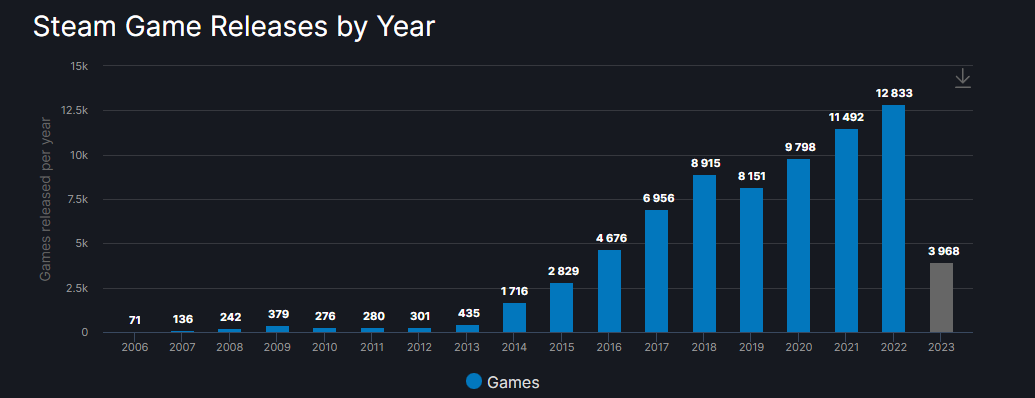
\includegraphics[scale=0.55]{./imagens/introducao/games_release_by_year.png}
	\caption{Steam Game Release Summary}
	\label{GameReleaseYear}
	\fonte{\cite{games_release_year}}
\end{figure}

Esse crescimento contínuo no mercado de jogos digitais é impulsionado pelo avanço tecnológico e pelo acesso generalizado à internet. A rápida penetração da internet na sociedade, como evidenciado por um estudo do \textit{\gls{DataReportal}}, mostra que aproximadamente 62,5\% da população mundial são usuários da internet, representando um aumento de 4\% em relação ao ano anterior \cite{digital_2022_global_overview_report}. No Brasil, o uso da internet está em constante ascensão, com pessoas entre 16 e 64 anos dedicando, em média, cerca de 10 horas diárias a atividades online \cite{digital_2022_global_overview_report}. O país se destaca como o terceiro no ranking mundial de tempo online, ficando atrás apenas da África do Sul e Filipinas, conforme evidenciado na Figura \ref{DailyTime}.

\begin{figure}[H]
	\centering
	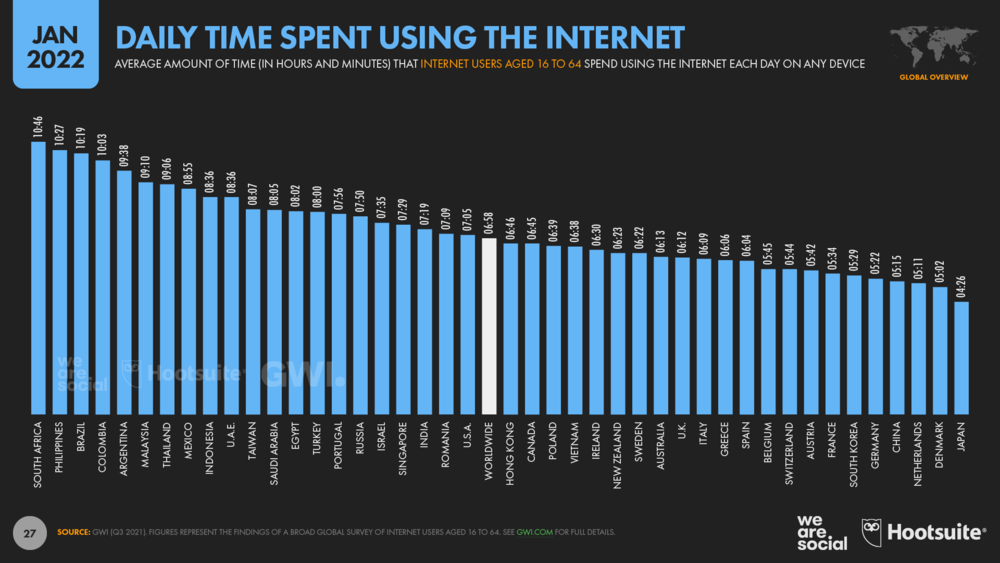
\includegraphics[scale=0.4]{imagens/introducao/daily_time_internet.png}
	\caption{Daily Time Spent Using The Internet}
	\label{DailyTime}
	\fonte{\cite{digital_2022_global_overview_report}}
\end{figure}

Esses dados indicam o Brasil como um mercado de grande potencial para produtos e conteúdos relacionados à internet, oferecendo um ambiente altamente favorável para iniciativas empreendedoras inovadoras. A mudança nos padrões de consumo, onde a conveniência e a acessibilidade proporcionadas pelas plataformas online desempenham um papel central, é particularmente evidente no cenário de jogos digitais. Este mercado em expansão, estimado em US\$ 323,5 bilhões até 2026 \cite{pesquisa_global_games}, requer soluções centralizadas para facilitar a gestão dos jogos para os entusiastas. Nesse contexto, a \textit{GameLocker} surge como uma solução ideal, não apenas para organizar os jogos, mas também para proporcionar um ambiente propício à interação entre jogadores, aproveitando ao máximo as oportunidades oferecidas por este mercado em expansão, as tendências atuais e se preparando para as futuras evoluções que certamente moldarão o futuro dos jogos eletrônicos.

% Proposta de solucao
\section{Proposta de Solução} 
\label{Proposta de Solução}

A introdução da aplicação \textit{GameLocker} resulta na implementação de um ambiente onde os jogadores podem administrar e sistematizar seus jogos de forma eficaz. Esta abordagem é facilitada pela funcionalidade de criar listas personalizadas e adaptáveis, permitindo ao jogador uma gestão organizada de sua coleção de jogos. Em adição a esse aspecto, o jogador tem a oportunidade de contribuir com suas avaliações e críticas pessoais sobre os jogos finalizados, fornecendo notas e análises escritas que enriquecem a experiência coletiva da comunidade.

Uma dimensão essencial da plataforma é o sistema de arenas de jogos, que alavanca a interação social e a competição entre os jogadores. Este sistema possibilita que os usuários integrem comunidades dedicadas a campeonatos, torneios e diversas modalidades de jogos em grupo. Nesse contexto, a comunidade se transforma em um ecossistema autossustentável, onde a interação entre os membros resulta em um ambiente envolvente e aconchegante.

A proposta da \textit{GameLocker} é proporcionar ao jogador um portal que englobe todas as funcionalidades indispensáveis para organização e descoberta de jogos, ao mesmo tempo em que incentiva a participação ativa na comunidade. Essa abordagem busca cultivar um espaço onde a organização se combina com a interação, onde as preferências individuais são partilhadas e onde o senso de comunidade é cultivado, proporcionando uma experiência aprimorada e uma base para o envolvimento constante dos jogadores.

% Concorrencia
    \section{Análise da Concorrência}

No processo de desenvolvimento deste projeto e na análise do mercado correspondente, foram identificada e examinadas     diversas aplicações com potencial concorrencial em relação ao \textit{GameLocker}. Nesse contexto, torna-se imprescindível a avaliação minuciosa destes concorrentes, visando à compreensão aprofundada de suas fraquezas e fortalezas. Simultaneamente, almeja-se a identificação das áreas nas quais a \textit{GameLocker} possui a oportunidade de se destacar perante esses competidores.

Ao apresentar a totalidade dos concorrentes devidamente elencados e detalhados no presente documento, emerge a identificação de dois competidores primordiais: os portais \textit{\gls{Alvanista}} e \textit{\gls{GGApp}}. Esta delimitação permite direcionar a análise de forma mais específica e concentrada, viabilizando uma investigação mais detalhada das estratégias e características que delineiam essas duas plataformas em relação à \textit{GameLocker}.

\subsection{Alvanista}

A plataforma \textit{\gls{Alvanista}} \cite{alvanista}, disponibilizada de forma gratuita, emerge como uma ferramenta de relevância incontestável. Ela se destaca ao proporcionar recursos essenciais, abrangendo a catalogação da biblioteca de jogos, a monitorização contínua do progresso individual do usuário, a viabilização de trocas de recomendações entre os participantes, a facilitação da imersão em comunidades de interesse específico e a facilitação da interconexão entre jogadores. A Figura \ref{Alvanista}, apresentada no formato próprio para ambiente online, proporciona uma representação visual da interface da plataforma. Esta imagem não apenas destaca a sua estrutura de maneira vívida, mas também evidencia a plenitude das funcionalidades incorporadas.

\begin{figure}[H]
	\centering
	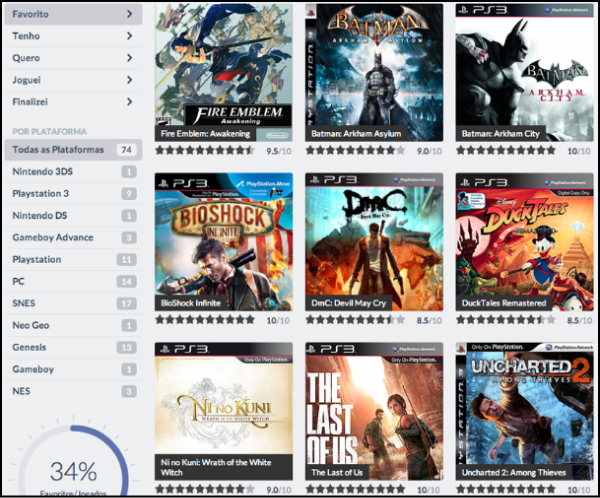
\includegraphics[scale=0.6]{./imagens/introducao/alvanista.png}
	\caption{Plataforma Alvanista}
	\label{Alvanista}
	Fonte: \cite{alvanista}
\end{figure}

A usabilidade deficiente torna a navegação pelo site complicada e confusa, dificultando a busca por informações e recursos importantes. Além da ausência de uma arena de jogos, a privação dos usuários da oportunidade de participarem de competições e desafios com outros jogadores. Tal ausência pode resultar em uma experiência menos emocionante e desestimular os usuários que buscam um ambiente competitivo.

\subsection{GG App}

O aplicativo móvel e a plataforma online \textit{\gls{GGApp}} \cite{ggapp}, como evidenciado na Figura \ref{ggapp}, apresentam-se como um conjunto integral, proporcionando uma gama diversificada de recursos destinados tanto à gestão eficaz de jogos quanto à promoção de interações entre os jogadores. Concebido com um propósito preciso, ele visa aprimorar a experiência dos jogadores, facilitando não apenas o controle das suas coleções de jogos, mas também incentivando a exploração de novos títulos, o estabelecimento de conexões com amigos e a imersão em comunidades virtuais.

\begin{figure}[H]
	\centering
	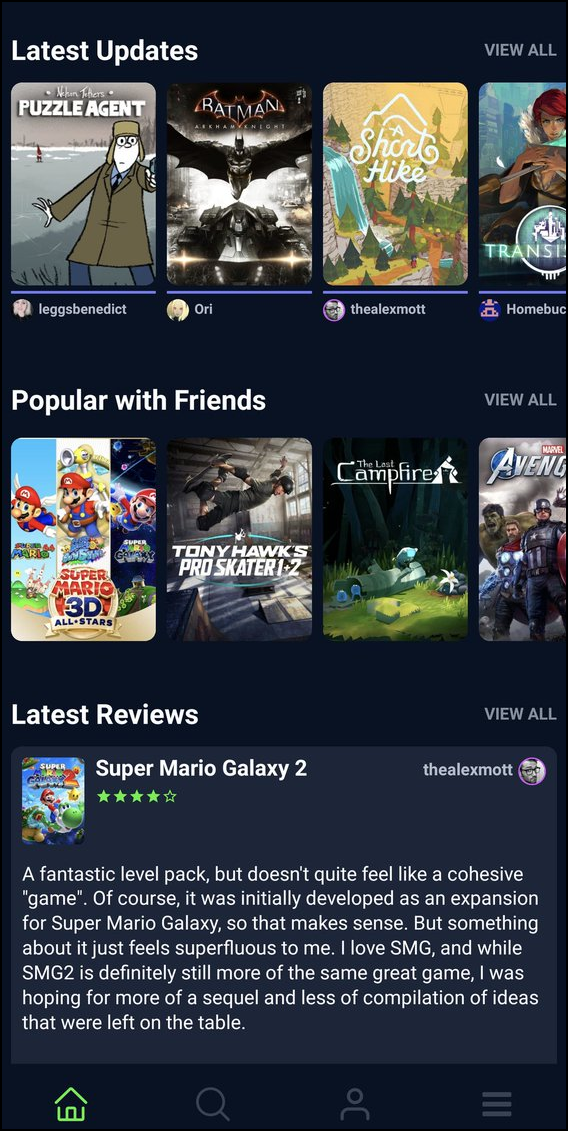
\includegraphics[scale=0.35]{./imagens/introducao/ggapp.png}
	\caption{Plataforma GG App}
	\label{ggapp}
	Fonte: \cite{ggapp}
\end{figure}

Uma arena de jogos oferece uma plataforma que possibilita aos jogadores interagirem entre si, seja por meio de chat ou em partidas competitivas. A ausência dessa funcionalidade pode resultar em uma experiência menos atraente para os usuários, com potencial para diminuição do engajamento, redução da interação social e dificuldades na medição de habilidades e promoção de jogos. A presença dessa arena promove uma atmosfera competitiva e socialmente interativa, encorajando a participação ativa dos usuários e incentivando melhorias contínuas nos jogos. Ademais, a falta dessa característica pode afetar negativamente a atratividade da plataforma perante outros serviços similares que fornecem esse recurso, afastando potenciais usuários em busca de uma experiência mais completa e imersiva.

\subsection{Comparação de Aplicativos Concorrentes}

Por meio das análises efetuadas, pôde-se constatar que tanto o \textit{\gls{Alvanista}} quanto o \textit{\gls{GGApp}} apresentam atributos que possibilitam a administração eficaz e a disseminação de avaliações relacionadas a jogos, além de propiciarem um ambiente propício para a interatividade entre seus usuários. No entanto, é relevante ressaltar que esses aplicativos não colocam uma ênfase significativa na criação de um espaço dedicado à competição direta entre os jogadores, conforme destacado no Quadro \ref{quadroConcorrente}.

\begin{quadro}[thb]
\centering
\ABNTEXfontereduzida
\caption{Comparação de Aplicativos Concorrentes}

\begin{tabular}{|l|c|c|c|}
\hline
\thead{Funcionalidades} & \thead{GameLocker} & 
\thead{Alvanista} & \thead{GG APP} \\
\hline
Usabilidade & X &  & X \
\\\hline
Gestão de jogos & X & X & X \
\\\hline
Avaliação de jogos & X & X & X \
\\\hline
Interação Social & X & X & X \
\\\hline
Arena de Jogos & X &  &  \
\\\hline
\end{tabular}
\label{quadroConcorrente}
\fonte{Autores}
\end{quadro}

No contexto das funcionalidades identificadas, torna-se evidente a preponderância das ferramentas destinadas à gestão e à comunicação, com ambas as plataformas fomentando a troca de análises críticas e opiniões acerca dos jogos. Essa ênfase demonstra a orientação compartilhada entre os concorrentes em direção a um ambiente colaborativo e informativo, onde os jogadores podem engajar-se em discussões enriquecedoras.

Entretanto, a distinção reside na ausência de um espaço especialmente dedicado à competição entre os usuários, algo que poderia acrescentar uma dimensão adicional à experiência oferecida. Tal ênfase, como identificada no Quadro \ref{quadroConcorrente}, é uma característica potencialmente diferenciadora que a \textit{GameLocker} pode explorar para se posicionar de forma distintiva no mercado, ao cativar um público que busca um ambiente não apenas para intercâmbio de informações, mas também para a competição saudável e a busca por reconhecimento no cenário dos jogos.

% Revisao de literatura
\chapter{Revisão da Literatura}

A finalidade desta revisão consiste em reunir e integrar investigações pertinentes relacionadas ao tema, as quais estão disponíveis na vasta literatura científica. Essa convergência tem como propósito primordial estabelecer uma base sólida e abrangente de conhecimento, contribuindo de forma simultânea para a solução dos desafios que emergiram durante o desenvolvimento desta pesquisa.

% O avanço tecnológico na sociedade moderna
\section{O avanço tecnológico na sociedade moderna}

A nomenclatura ``era da tecnologia'' ganhou relevância nos últimos anos ao descrever o período contemporâneo em que a humanidade está imersa, onde inúmeras atividades cotidianas são não apenas assistidas, mas, em alguns casos, substancialmente dependentes das maravilhas tecnológicas. Dentro desta linha de pensamento, emerge com notoriedade a importância da Internet, que figura como uma força condutora ao possibilitar avanços notáveis em um lapso temporal reduzido. Concebida pelo cientista britânico \textit{Tim Berners-Lee} em 1989, a Internet remodelou por completo o panorama das comunicações, sendo que, apesar de sua criação relativamente recente, evoluiu para se tornar um epicentro impulsionador de uma metamorfose sem precedentes, ilustrada vividamente na Figura \ref{GlobalInternetUsers}.

\begin{figure}[H]
	\centering
	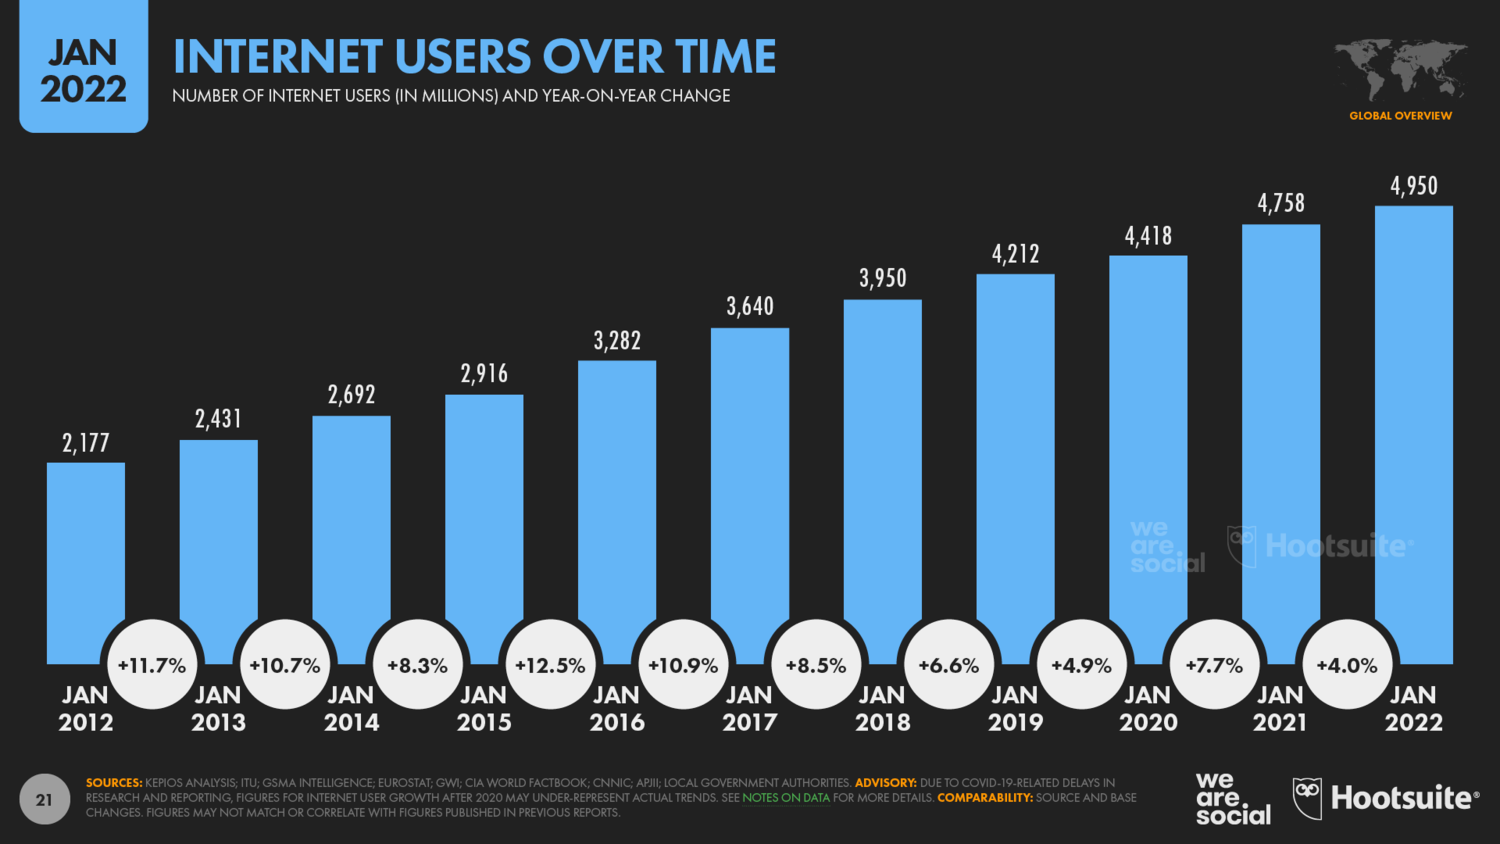
\includegraphics[scale=0.3]{imagens/revisaoLeitura/global_internet_users_over.png}
	\caption{Global Internet Users Over }
	\label{GlobalInternetUsers}
	\fonte{\cite{digital_2022_global_overview_report}}
\end{figure}

Na era tecnológica, a Internet emerge como uma influência transformadora, conectando bilhões de pessoas globalmente e desempenhando um papel central em várias esferas da vida humana. Seu impacto persistirá, moldando o mundo à medida que novas tecnologias e inovações surgem, promovendo um futuro cada vez mais interconectado e globalizado para a humanidade.



% Mercado de jogos
\section{Mercado de jogos}

A indústria de jogos eletrônicos está passando por um crescimento contínuo, impulsionada pelos avanços tecnológicos e pelas mudanças nas preferências dos consumidores. De acordo com um estudo conduzido pela empresa \textit{\gls{Newzoo}}, as projeções para o mercado global de jogos indicam um aumento aproximado de 3.4\% até o ano de 2025. Esse crescimento representa um potencial de lucro estimado em cerca de US\$ 211.2 bilhões em escala mundial, destacando o apelo universal dos jogos eletrônicos que ultrapassam barreiras culturais e geográficas, conforme ilustrado na Figura \ref{GlobalMarketForecast}.

A diversificação do público consumidor, incluindo crianças, adultos e idosos, tem gerado uma demanda crescente por uma variedade de jogos. Além disso, tendências como jogos \textit{\gls{Multiplayer}} online e jogos baseados em computação em nuvem, bem como avanços tecnológicos, como gráficos de alta qualidade, realidade virtual e dispositivos móveis poderosos, têm aumentado a acessibilidade aos jogos eletrônicos, contribuindo significativamente para a expansão do mercado.

\begin{figure}[H]
	\centering
	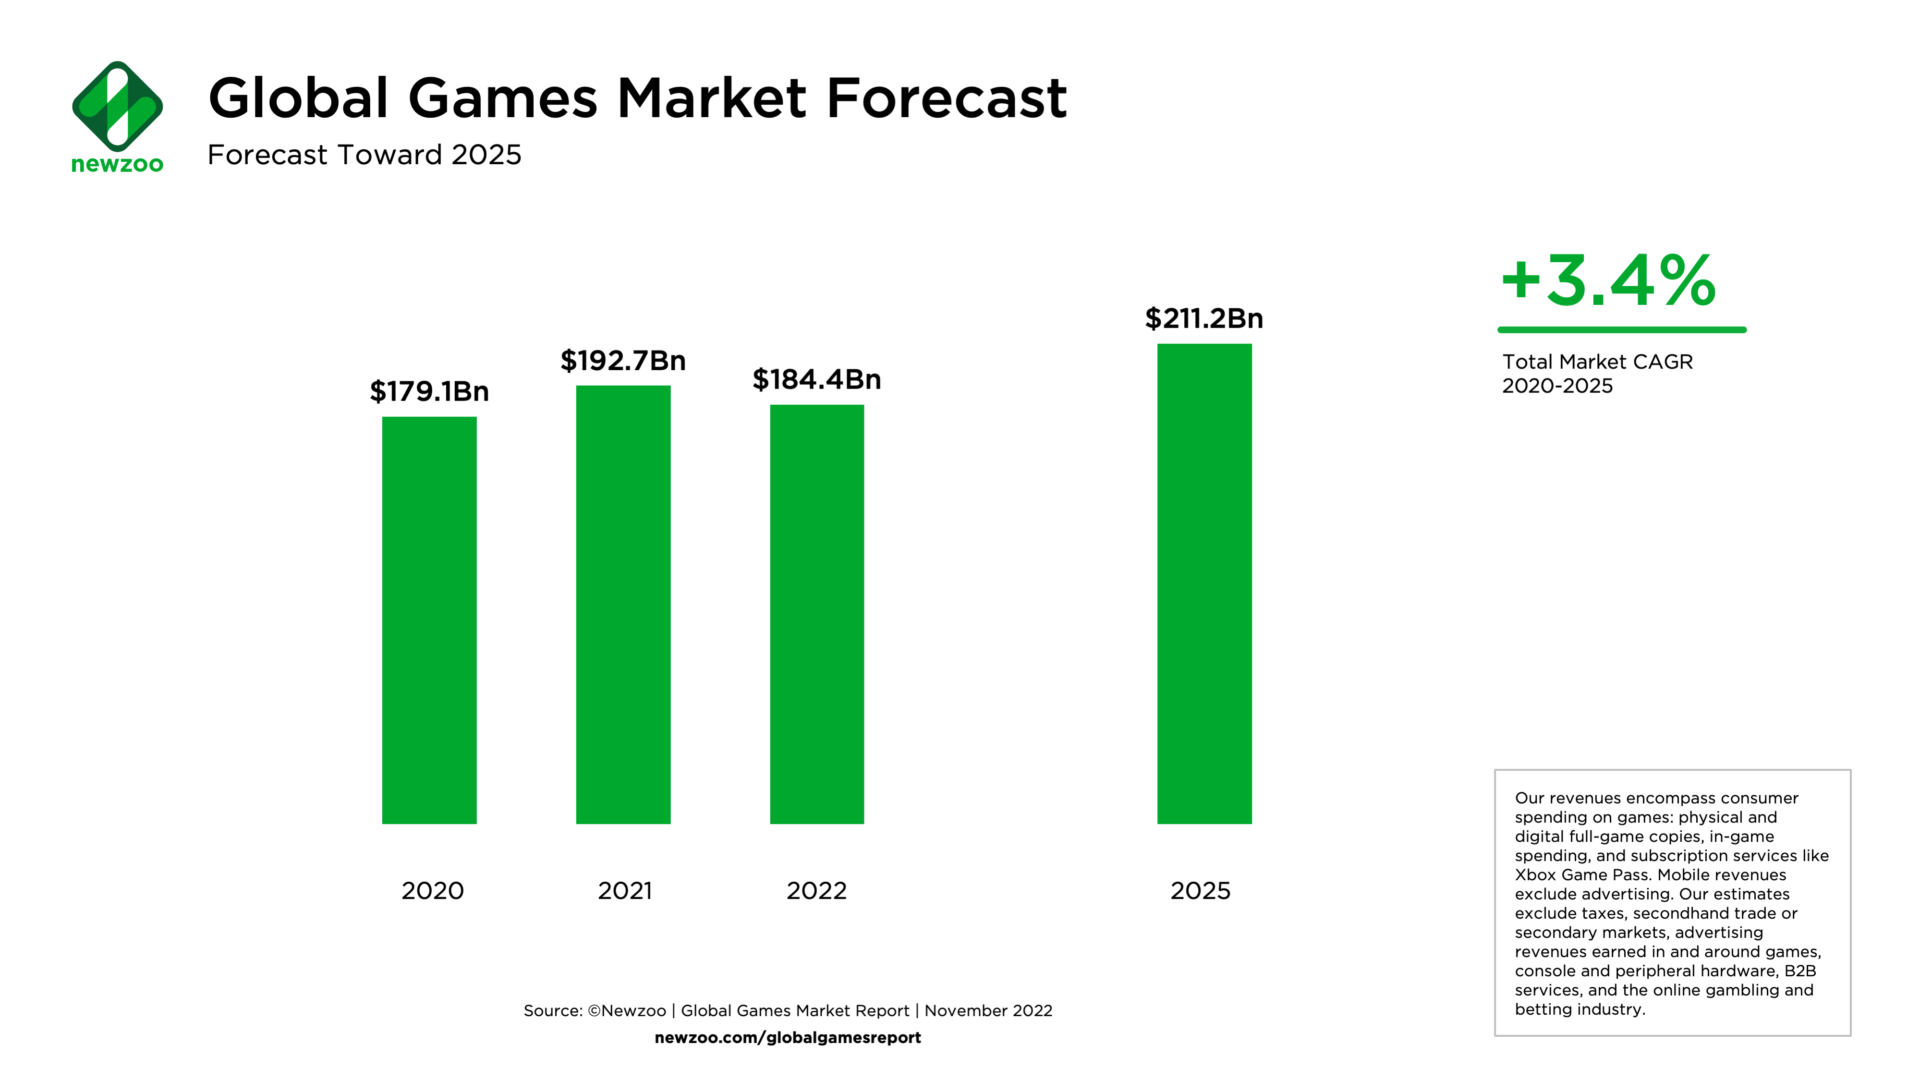
\includegraphics[scale=0.24]{imagens/revisaoLeitura/global_games_market_forecast.png}
	\caption{Global Market Forecast}
	\label{GlobalMarketForecast}
	\fonte{\cite{global_games_market}}
\end{figure}

Além de seu valor de entretenimento, a indústria de jogos eletrônicos possui impactos econômicos e sociais notáveis. O mercado de \textit{eSports} está crescendo exponencialmente, criando empregos para jogadores profissionais e profissionais relacionados. Socialmente, os jogos eletrônicos desempenham um papel crucial na formação de comunidades online, oferecendo um sentido de pertencimento e camaradagem em um mundo digitalizado.

O futuro da indústria de jogos eletrônicos é promissor, com a integração da inteligência artificial e tecnologias de aprendizado de máquina prometendo jogos mais dinâmicos e adaptativos. Além disso, a realidade aumentada está gerando experiências inovadoras que combinam o mundo físico e digital, indicando um caminho empolgante para a evolução dos jogos eletrônicos.

Para compreender plenamente a magnitude dessa cifra substancial, torna-se imperativo realizar uma comparação com setores de entretenimento mais consolidados, como a indústria cinematográfica e musical. Segundo dados da \textit{\gls{GrandViewResearch}}, esses setores alcançaram lucros na ordem de US\$ 90.1 bilhões, conforme evidenciado na Figura \ref{GlobalMoviesEntertainmentMarket}. A disparidade financeira entre os jogos eletrônicos e esses segmentos tradicionais ressalta a ascensão meteórica dos jogos na economia global, traçando um cenário claro e incontestável da crescente importância econômica dos videogames.

\begin{figure}[H]
	\centering
	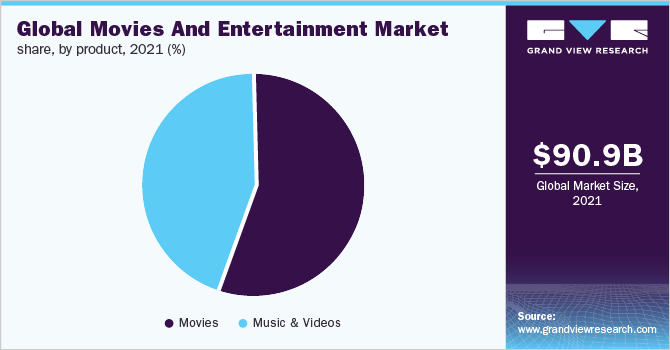
\includegraphics[scale=0.6]{imagens/revisaoLeitura/global_movies_entertainment_market.png}
	\caption{Global Movies Entertainment Market}
	\label{GlobalMoviesEntertainmentMarket}
	\fonte{\cite{global_films_musics_market}}
\end{figure}

A indústria cinematográfica, que já foi considerada um dos pilares fundamentais do entretenimento, agora enfrenta uma concorrência acirrada dos jogos eletrônicos. Esta transformação evidencia as preferências dos consumidores, e a capacidade dos jogos eletrônicos de se adaptarem às mudanças tecnológicas, oferecendo experiências interativas e imersivas que atraem públicos de todas as idades.

No campo da música, historicamente uma das formas de entretenimento mais lucrativas, os videogames também estão fazendo incursões significativas. A trilha sonora de jogos, muitas vezes composta por músicas originais e licenciadas, tornou-se uma parte integral da experiência de jogo. Além disso, eventos e competições de jogos eletrônicos frequentemente apresentam performances ao vivo de artistas musicais renomados, criando uma sinergia entre os dois mundos do entretenimento e ampliando ainda mais o alcance dos jogos eletrônicos. 

Nesse panorama, convém salientar que o êxito financeiro do mercado de jogos ultrapassa o resultado de um segmento isolado, consistindo, da complexa interação entre diversos setores dentro da indústria de jogos. A análise desses segmentos revela uma gama abrangente de possibilidades, incluindo Jogos de Computador, Consoles, Plataformas Móveis e Navegadores, todos contribuindo de maneiras distintas para a expansão contínua do mercado.

Um aspecto que merece destaque é a crescente importância dos jogos para dispositivos móveis nesse cenário multifacetado. Pesquisas recentes conduzidas pela renomada empresa \textit{\gls{Newzoo}} demonstram de forma clara que o setor de jogos para dispositivos móveis está destinado a liderar essa expansão. A Figura \ref{GlobalMarketPerSegment}, que corrobora essas descobertas, revela uma tendência ascendente notável nesse segmento específico da indústria de jogos.

\begin{figure}[H]
	\centering
	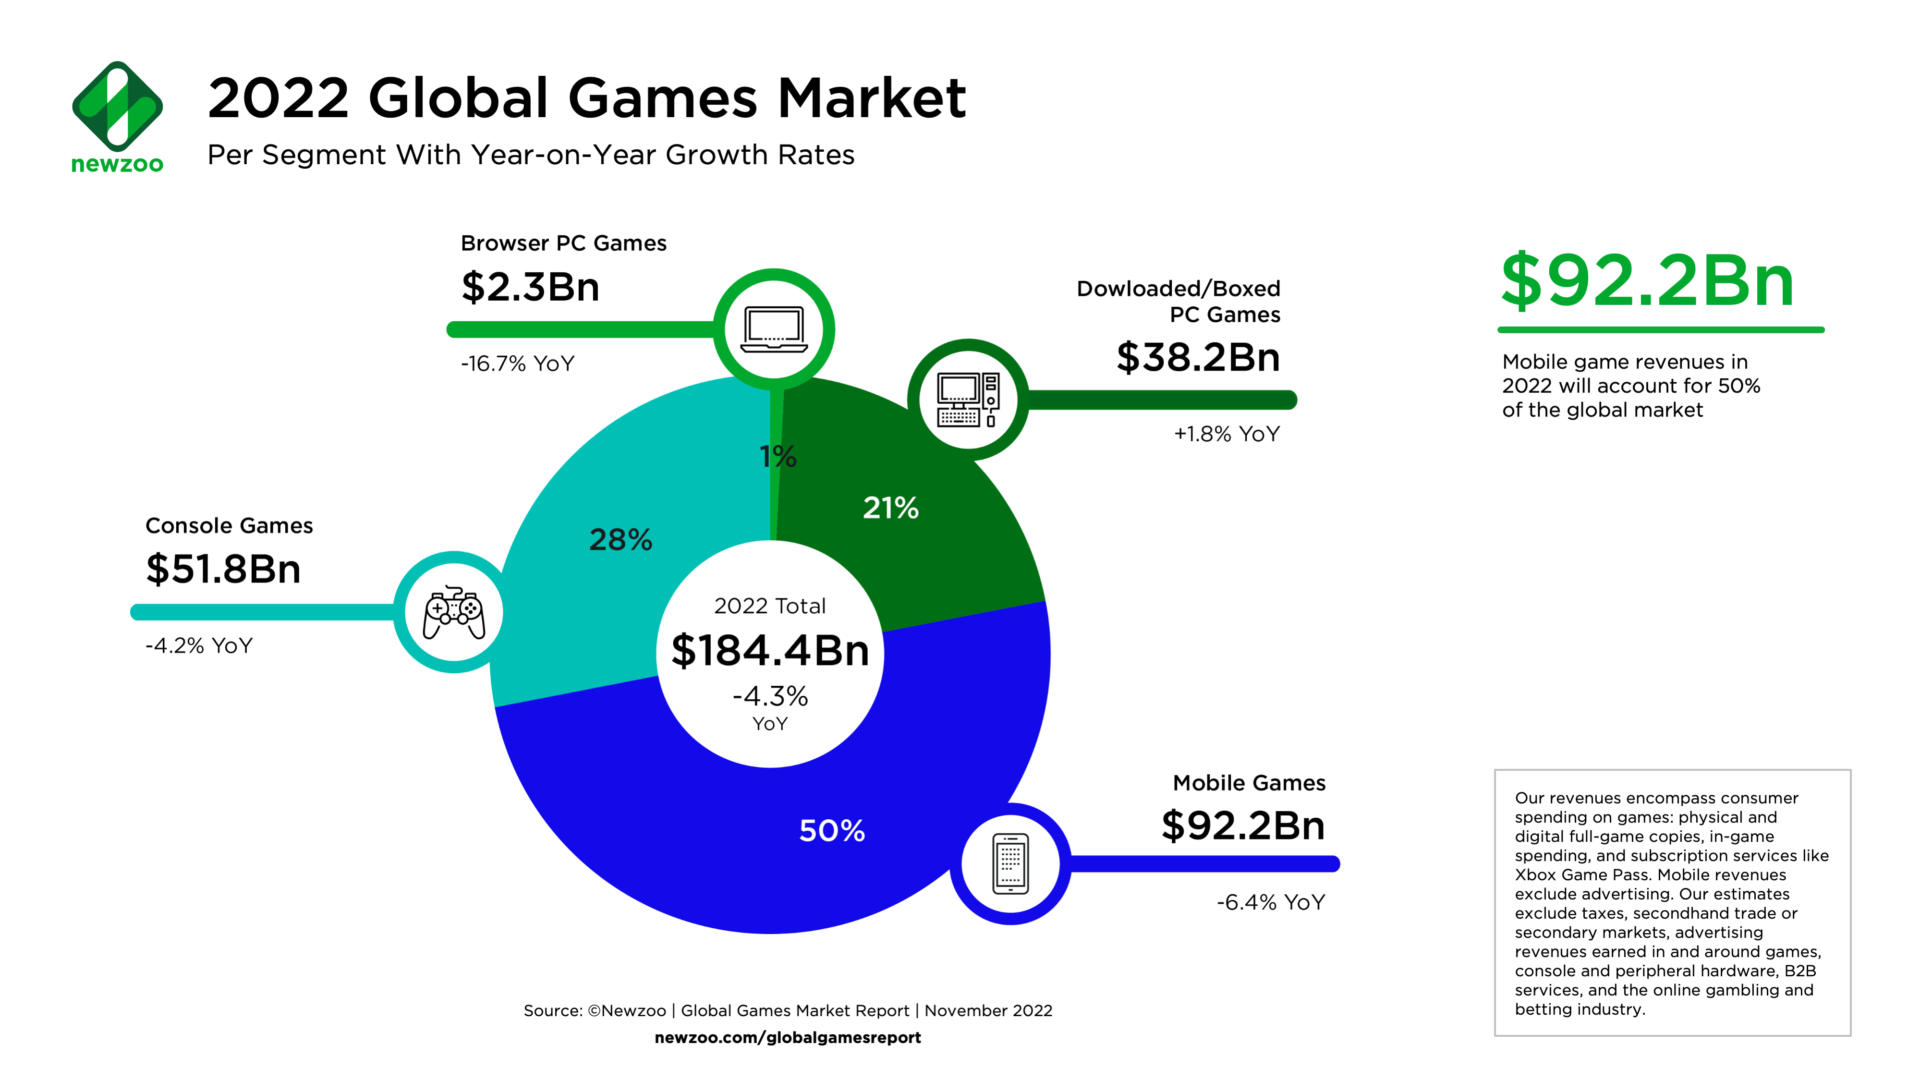
\includegraphics[scale=0.22]{imagens/revisaoLeitura/global_games_market_per_segment.png}
	\caption{Global Market Per Segment}
	\label{GlobalMarketPerSegment}
	\fonte{\cite{global_games_market}}
\end{figure}

A relevância desse crescimento exponencial no mercado de jogos móveis é inegável. Não apenas os dispositivos móveis estão cada vez mais acessíveis, mas também oferecem uma plataforma altamente conveniente para os jogadores, que podem desfrutar de uma variedade de jogos com apenas alguns toques na tela de seus \textit{smartphones} ou \textit{tablets}. Essa acessibilidade instantânea atrai os jogadores casuais, e cativa uma base de jogadores mais dedicada e ávida por experiências de alta qualidade.

Além disso, é fundamental notar que a diversificação de plataformas facilita o acesso aos jogos, e impulsiona a inovação na indústria. Desenvolvedores de jogos agora têm a oportunidade de explorar novas tecnologias e ideias em diferentes plataformas, levando a uma riqueza de opções para os consumidores. Essa competição saudável entre os segmentos da indústria de jogos resulta em uma ampla gama de produtos, desde jogos independentes inovadores até títulos \textit{\gls{AAA}} de grande orçamento, todos contribuindo para a riqueza e diversidade do mercado.

% Plataforma de distribuição de jogos
\section{Plataformas de Distribuição de Jogos}

As Plataformas de Distribuição de Jogos representam os ambientes virtuais onde jogadores podem adquirir seus jogos de maneira digital. Uma pesquisa conduzida pela empresa \cite{games_distribution_platform}, especializada em análise de dados e tecnologia com sede no Reino Unido, aponta que as principais plataformas de distribuição são a \textit{\gls{Steam}} \textit{(\gls{Valve})}, a \textit{\gls{Origin}} \textit{(\ac{ea})} e a \textit{\gls{Battle-Net}} \textit{(\gls{Blizzard})}).

Algumas destas plataformas vão além da mera distribuição e oferecem funcionalidades adicionais, como gerenciamento de bibliotecas e integração de serviços. Um exemplo é a \textit{Epic Games Store}, que introduziu o \textit{Epic Gaming Manager}, um aplicativo de gerenciamento que proporciona aos jogadores uma experiência centralizada para acessar e atualizar seus jogos disponíveis na loja. Ademais, a plataforma \textit{Epic Online Services}, uma suíte de ferramentas e serviços que capacita os desenvolvedores de jogos a criar, lançar e gerenciar experiências interativas online \textit{multiplayer} e outros tipos de jogos. A plataforma oferece uma variedade de recursos, incluindo gerenciamento de identidade e contas, com soluções seguras para autenticação de jogadores e gestão de perfis de jogador. Além disso, conta com um sofisticado sistema de \textit{matchmaking} que permite aos jogadores encontrar partidas com outros jogadores que possuem habilidades e preferências semelhantes. 

\subsection{Steam}

A \textit{\gls{Steam}}, lançada pela \textit{\gls{Valve} Corporation} em 2003, se coloca como uma plataforma de jogos online de destaque. Ela emerge como uma das maiores plataformas de distribuição digital de jogos para PC a nível global, conferindo aos usuários uma extensa gama de funcionalidades. Através da \textit{\gls{Steam}}, os jogadores podem adquirir e fazer \textit{download} direto dos jogos em seus computadores, e recebem atualizações automáticas sempre que novas versões são lançadas. A plataforma também agrega elementos sociais, incluindo a possibilidade de adicionar amigos, integrar-se a grupos e participar de bate-papos, fomentando a interconexão entre jogadores ao redor do mundo.

A grande diversidade de títulos é uma das proeminentes vantagens da \textit{\gls{Steam}}, que oferece uma biblioteca com mais de 30.000 jogos disponíveis para \textit{download}, abarcando tanto títulos \textit{\gls{AAA}} quanto independentes. Somado a isso, a \textit{\gls{Steam}} regularmente oferece promoções e descontos em jogos, democratizando o acesso aos jogadores de todas as vertentes.

\subsection{Origin}

A \textit{\gls{Origin}}, desenvolvida pela \ac{ea}, uma das maiores empresas globais de entretenimento interativo, proporciona aos jogadores uma plataforma de distribuição digital de jogos. O intuito da \textit{\gls{Origin}} é conferir aos jogadores uma experiência acessível e cômoda para aquisição e jogo de seus jogos preferidos em seus computadores.

Através da \textit{\gls{Origin}}, os usuários obtêm acesso a uma variada gama de jogos, incorporando títulos \textit{\gls{AAA}} e independentes, além de DLCs, demonstrações e jogos gratuitos. Uma característica distintiva da plataforma é o seu \textit{feed} social, semelhante a redes sociais, permitindo que os jogadores sigam amigos e compartilhem suas conquistas nos jogos. Além disso, a \textit{\gls{Origin}} oferece notificações de descontos e oportunidades para experimentar versões beta exclusivas de jogos antes do lançamento oficial. A plataforma garante ainda atualizações automáticas para assegurar que os jogos estejam sempre atualizados e funcionando devidamente.

\subsection{Battle-Net}

Desenvolvida pela \textit{\gls{Blizzard} Entertainment}, uma das principais empresas do mundo dos jogos, a \textit{\gls{Battle-Net}} proporciona aos jogadores uma plataforma que almeja facilitar a jogabilidade de seus jogos mais renomados, incluindo títulos como \textit{World of Warcraft}, \textit{Diablo}, \textit{Overwatch} e \textit{Starcraft}.

Através da \textit{\gls{Battle-Net}}, os jogadores se deparam com uma série de recursos, englobando jogos, fóruns, lojas online e serviços de suporte. As opções de jogo são variadas, permitindo partidas online com outros jogadores ou jogar individualmente. Um fator notável da plataforma é o foco na segurança, com um sistema de autenticação sólido que resguarda as contas dos jogadores contra atividades fraudulentas.

% Planejamento e gerenciamento
\chapter{Gerenciamento do Projeto}

A fim de assegurar a entrega do projeto no prazo e orçamento estabelecidos, bem como melhorar a eficiência operacional, torna-se imprescindível estabelecer características essenciais para o planejamento, execução, monitoramento e controle do projeto. A aplicação dessas práticas permite garantir que o projeto atenda às demandas empresariais e seja concluído com a qualidade necessária para alcançar os resultados esperados.

% Metodologia de gestao
\section{Metodologia de Gestão de Projeto}

A seleção da metodologia ágil de gestão de projetos \textit{\gls{Kanban}} foi feita devido à sua notável capacidade de gerenciar eficazmente mudanças e incertezas ao longo do projeto. Com o intuito de promover a coesão, alinhamento e colaboração harmônica entre os membros da equipe, são empregadas ferramentas essenciais que garantem o pleno funcionamento do processo. As seguintes ferramentas desempenham papéis fundamentais nesse contexto:

Para viabilizar reuniões e discussões eficientes, a plataforma \textit{\gls{Discord}} é adotada como meio principal. Ela proporciona um ambiente virtual propício para a interação e troca de ideias entre os participantes do projeto. Através do \textit{\gls{Discord}}, é possível promover debates construtivos e manter a equipe atualizada sobre os progressos e desafios do projeto.

Com o propósito de agilizar a comunicação e facilitar a resolução imediata de dúvidas, o aplicativo \textit{\gls{Whatsapp}} é utilizado. Essa ferramenta se mostra valiosa para estabelecer conexões rápidas entre os membros da equipe, permitindo a rápida troca de informações e esclarecimentos pontuais.

Para a divulgação das atividades executadas e o compartilhamento de informações relevantes, o \textit{\gls{Blog}} assume um papel crucial. Essa plataforma online serve como um espaço dedicado à documentação das etapas cumpridas, permitindo que os membros da equipe acompanhem o desenvolvimento do projeto de forma transparente e estruturada.

O \textit{\gls{Jira}} é a plataforma eleita para a distribuição e controle das tarefas, como representado na figura \ref{Jira}. Esta ferramenta centraliza a atribuição de responsabilidades, facilitando o acompanhamento do status de cada atividade. O \textit{\gls{Jira}} não apenas contribui para a organização eficaz, mas também para a identificação de possíveis gargalos e atrasos, possibilitando ações corretivas oportunas.

\begin{figure}[H]
	\centering
	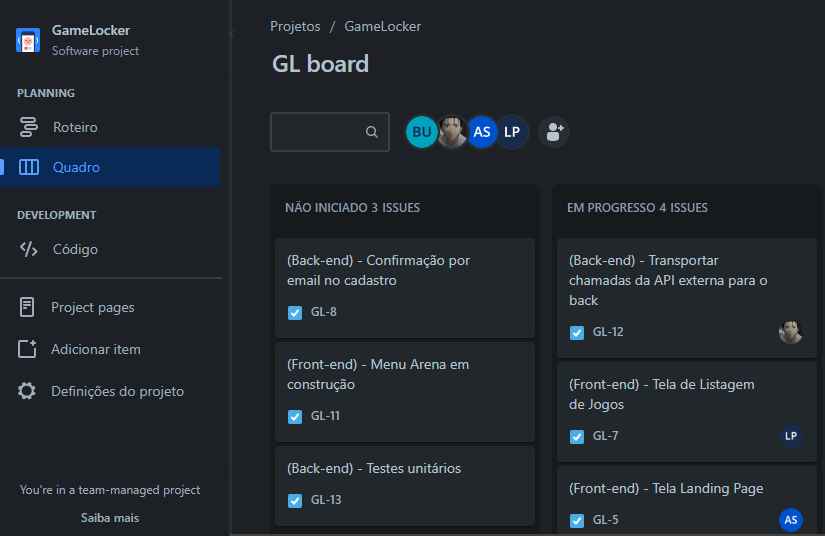
\includegraphics[scale=0.6]{imagens/planejamentoGerenciamento/jira.png}
	\caption{Jira}
	\label{Jira}
	\fonte{Autores}
\end{figure}



% Sprint
\section{Gestão de Tempo}

Foi estabelecido um cronograma de encontros presenciais de curta duração, agendados às quintas-feiras, com o propósito de discutir as pendências e monitorar o progresso do projeto. Adicionalmente, em situações de urgência, programadas reuniões adicionais aos finais de semana para abordar questões críticas que demandem atenção imediata.

Durante as reuniões, são realizadas revisões abrangentes das tarefas em andamento, com o objetivo de identificar gargalos, determinar as prioridades de desenvolvimento e explorar oportunidades de colaboração entre os membros da equipe.

% Organizacao da equipe
\section{Organização da equipe}

A equipe de projeto GameLocker, é formada por integrantes do curso de Análise e Desenvolvimento de Sistemas do \ac{ifsp}. A seguir uma breve descrição do perfil de cada integrante:

\begin{itemize}

\item \textbf{Alisson Kauan da Silva Santos}: Atualmente, ocupa a posição de estagiário de desenvolvimento \textit{\gls{Back-end}} na Unisys: Soluções de Tecnologia. Principal responsabilidade, trabalhar com o \textit{\gls{Framework}} \textit{\gls{.NET}} para a linguagem de programação \textit{\gls{Csharp}}, além de lidar com o banco de dados \textit{\gls{Sqlserver}}. Interesse e entusiasmo pelo desenvolvimento de sistemas;

\item \textbf{Brayan Yukio Uehara}: Atualmente, ocupa a função de Desenvolvedor de Software \textit{\gls{FullStack}} na empresa SATO Brasil, utiliza-se um conjunto diversificado de tecnologias para criar soluções eficazes. Principais áreas de atuação incluem o desenvolvimento de aplicativos e sistemas utilizando as linguagens de programação \textit{\gls{Csharp}}, \textit{\gls{Lua}} e \textit{\gls{Python}};

\item \textbf{Iuri Nicolas Henrique Garcia}: Atualmente, ocupa a função de estagiário em desenvolvimento de software \textit{\gls{FullStack}} na empresa itBeta², utilizando ferramentas como \textit{\gls{JavaSpring}}, \textit{\gls{MySQL}} e \textit{\gls{Angular}} para o desenvolvimento de aplicações Web. Auxilia também nas decisões sobre interfaces visuais nos projetos. Possui interesse maior por desenvolvimento \textit{\gls{Front-end}};

\item \textbf{Lucas de Lima Passos}: Atualmente, desempenha a função de Desenvolvedor Web e Mobile Júnior no Grupo GCB. Dentro dessa posição, se concentra no desenvolvimento de aplicações web utilizando a biblioteca \textit{\gls{React}}, bem como no desenvolvimento de aplicativos mobile usando o \textit{\gls{Framework}} \textit{\gls{ReactNative}}. Possui interesse particular no desenvolvimento mobile;

\item \textbf{Pedro Henrique Farias Boscachi}: Atualmente, ocupa a posição de estagiário de desenvolvimento \textit{\gls{FullStack}} na empresa BtCréditos. Trabalha com o \textit{\gls{Framework}} \textit{\gls{.NET}} para a linguagem de programação \textit{\gls{Csharp}} e com o banco de dados \textit{\gls{Sqlserver}}. Possui interesse significativo na área de desenvolvimento de sistemas.

\item \textbf{Rodrigo Shimizu Passos}: Atualmente, atua como estagiário em desenvolvimento de software \textit{\gls{FullStack}} na empresa itBeta², trabalhando com ferramentas como \textit{\gls{JavaSpring}}, \textit{\gls{MySQL}} e \textit{\gls{Angular}} no desenvolvimento de aplicações Web. Por vezes, auxilia na descoberta de requisitos nos projetos. Possui interesse particular por desenvolvimento \textit{\gls{Back-end}};

\end{itemize}

No contexto do projeto, as tarefas são divididas e atribuídas levando em consideração as disponibilidades de recursos e as habilidades dos integrantes da equipe, conforme o Quadro \ref{quadroOrganizacaoEquipe}.

\begin{quadro}[thb]
\centering
\ABNTEXfontereduzida
\caption{Organização da equipe}

\begin{tabular}{|l|c|c|c|c|c|c|}
\hline
\thead{Integrantes} & \thead{Alisson} & 
\thead{Brayan} & \thead{Iuri} & \thead{Lucas} & \thead{Pedro} & \thead{Rodrigo}\\
\hline
Back-end &  & X &  &  & X & X \
\\\hline
Blog &  & X &  &  & X & X \
\\\hline
Front-end & X &  & X & X &  &  \
\\\hline
Gestão & X & X & X & X & X & X  \
\\\hline
Documentação &  & X &  &  &  & X  \
\\\hline
\end{tabular}
\label{quadroOrganizacaoEquipe}
\fonte{Autores}
\end{quadro}

A equipe responsável pelo projeto colabora em conjunto para garantir a qualidade e eficiência de todas as etapas. Brayan, Pedro e Rodrigo assumem a responsabilidade pelo desenvolvimento do \textit{\gls{Back-end}}, onde se realiza a criação da \ac{api}, e na integração do banco de dados com a plataforma de nuvem \textit{\gls{Azure}}. Alisson, Lucas e Iuri são encarregados da programação do  \textit{\gls{Front-end}} e pela \ac{ux}/\ac{ui} do projeto.

No que tange à manutenção e atualização constante do Blog, Brayan, Pedro e Rodrigo assumem a importante missão de garantir que o conteúdo seja regularmente revisado e atualizado, garantindo a transparência e coerência das informações.

Em relação à documentação integral do projeto, todos os integrantes contribuem, todavia, Brayan e Rodrigo carregam a responsabilidade preponderante na adequação da documentação, garantindo que ela se alinhe com os padrões estabelecidos. 

A gestão deve ser realizada por todos os membros, garantindo que estejam alinhados com suas respectivas tarefas e contribuam no registro das atividades e dos processos de desenvolvimento.

% ARQUITETURA E TECNOLOGIA Arquitetura e tecnlogia
\chapter{Arquitetura e Tecnologias}

No presente tópico, são definidas e detalhadas todas as partes que envolvem a arquitetura e tecnologias utilizadas no sistema. Nesse sentido, modelos visuais foram criados com o propósito de proporcionar um melhor entendimento e assimilação do funcionamento do sistema.

\section{Escopo do Projeto}

No escopo, busca-se compreender a extensão do projeto e todas as partes abrangidas por ele, tanto no âmbito do negócio quanto no âmbito do desenvolvimento. Adicionalmente, são destacadas as metas e objetivos do desenvolvimento nesta seção.

% Requisitos
\subsection{Requisitos}

Neste tópico, são analisados e definidos os fatores de negócio do projeto, tais como requisitos funcionais, requisitos não funcionais, regras de negócio, histórias de usuários e possíveis casos de uso. Todos esses fatores foram considerados para o desenvolvimento do projeto e devem ser seguidos de maneira objetiva e concreta. É importante ressaltar que determinados requisitos e histórias podem sofrer alterações no futuro, uma vez que mudanças no projeto podem ocorrer.

% Regras de negócio
\subsubsection{Regras de Negócio}
\label{sec:regras_negocio}

Os Quadros \ref{tab:regrasdenegocio1}, \ref{tab:regrasdenegocio2} e \ref{tab:regrasdenegocio3} estão organizados por temas, com o propósito de aprimorar a organização e a compreensão do conteúdo. Estes quadros têm como objetivo descrever de maneira abrangente todas as regras de negócio propostas, as quais devem ser integralmente incorporadas nos requisitos funcionais e não funcionais do projeto.

\begin{quadro}[h!]
\centering
\caption{Regras de Negócio de Login, Autenticação e Usuário}
\label{tab:regrasdenegocio1}
\begin{longtable}{|p{2.5cm}|p{10.0cm}|p{2.5cm}|}
\hline
ID & Descrição & Relacionados
\\\hline
RN1 & Ao acessar o site, para ter acesso aos conteúdos e funcionalidades, o usuário deve estar previamente autenticado &  \
\\\hline
RN2 & O acesso do usuário ao sistema de login é restrito àqueles que possuem um cadastro ativo &  \
\\\hline
RN3 & Durante o processo de cadastro, é imprescindível que o usuário confirme seu endereço de e-mail a fim de validar seu registro &  \
\\\hline
RN4 & Deve ser enviado um e-mail para redefinição de senhas de usuários &  \
\\\hline
RN5 & Cada usuário deve possuir um perfil individual, através do qual poderá administrar seus dados pessoais e informações relacionadas aos jogos &  \
\\\hline
RN6 & O usuário possui a prerrogativa de editar seus próprios dados pessoais &  \
\\\hline
RN7 & É facultado ao usuário o direito de excluir sua conta a qualquer momento &  \
\\\hline
\end{longtable}
\fonte{Os Autores.}
\end{quadro}

\begin{quadro}[h!]
\centering
\caption{Regras de Negócio de Gerenciamento de Jogos e Assinatura Premium}
\label{tab:regrasdenegocio2}
\begin{longtable}{|p{2.5cm}|p{10.0cm}|p{2.5cm}|}
\hline
ID & Descrição & Relacionados
\\\hline
RN8 & Ao selecionar um jogo, o usuário tem a possibilidade de adicioná-lo ao seu perfil &  \
\\\hline
RN9 & No momento de adicionar o jogo, é exigido que o usuário forneça informações básicas sobre o jogo &  \
\\\hline
RN10 & Após a inclusão, o usuário terá permissão para editar as informações dos seus jogos &  \
\\\hline
RN11 & No perfil do usuário, devem estar disponíveis todas as listagens de jogos, organizadas com base em seu status &  \
\\\hline
RN12 & Os usuários devem ter a capacidade de visualizar todos os jogos e avaliações nos perfis de outros usuários &  \
\\\hline
RN13 & O usuário terá a opção de filtrar os jogos com base em determinados parâmetros &  \
\\\hline
RN14 & O usuário deve ser capaz de avaliar um jogo, atribuindo uma nota e fornecendo uma crítica &  \
\\\hline
RN15 & O usuário deve ter a capacidade de excluir os jogos que adicionou a qualquer momento &  \
\\\hline
RN16 & Os usuários serão categorizados em usuários comuns e usuários premium &  \
\\\hline
RN17 & O sistema deve incorporar um modelo de assinatura premium, onde os usuários que pagarem uma quantia específica terão acesso a determinados benefícios e funcionalidades exclusivas &  \
\\\hline
RN18 & Usuários comuns não terão acesso a benefícios extras &  \
\\\hline
RN19 & Os usuários premium têm o direito de cancelar sua assinatura a qualquer momento &  \
\\\hline
\end{longtable}
\fonte{Os Autores.}
\end{quadro}


\begin{quadro}
\centering
\caption{Regras de Negócio da Arena de Jogos}
\label{tab:regrasdenegocio3}
\begin{longtable}{|p{2.5cm}|p{10.0cm}|p{2.5cm}|}
\hline
ID & Descrição & Relacionados
\\\hline
RN20 & O sistema deve oferecer uma aba dedicada às arenas &  \
\\\hline
RN21 & Cada arena deve possuir um administrador designado, sendo restrito aos usuários premium o direito de se tornarem administradores de arenas &  \
\\\hline
RN22 & Ao criar uma arena, o administrador é responsável por definir informações essenciais, como o jogo a ser jogado e a descrição da arena &  \
\\\hline
RN23 & O administrador tem a autorização para excluir sua arena a qualquer momento &  \
\\\hline
RN24 & Cada arena contará com um chat exclusivo, permitindo a comunicação entre todos os jogadores presentes na arena &  \
\\\hline
\end{longtable}
\fonte{Os Autores.}
\end{quadro}
\pagebreak

% Requisitos funcionais
\clearpage
\subsubsection{Requisitos Funcionais}
\label{sec:req_funcionais}

Neste capítulo, apresentam-se os requisitos indispensáveis à garantia de usabilidade e prestação de serviço abrangente aos usuários da aplicação. A síntese destes requisitos é fornecida nos Quadros \ref{tab:requisitosfuncionais1} e \ref{tab:requisitosfuncionais2}, onde se estabelece uma visão panorâmica dessas demandas. Estes quadros contextualizam os requisitos com as regras de negócio correspondentes e destacam a sua relevância no contexto do desenvolvimento, crucial para assegurar o sucesso do projeto.

\begin{quadro}[h!]
\caption{Requisitos Funcionais de Login, Usuário e Gerenciamento de Jogos}
\label{tab:requisitosfuncionais1}
\begin{longtable}{|p{2.5cm}|p{7.5cm}|p{2.5cm}|p{2.5cm}|}
\hline
ID & Descrição & Importância & Relacionados
\\\hline
RF1 & O sistema deve permitir que novos usuários realizem o cadastro & Alta & RN3 \
\\\hline
RF2 & O sistema deve permitir que os usuários realizem o login & Alta & RN2 \
\\\hline
RF3 & O sistema deve ser capaz de enviar um e-mail para confirmação de conta & Alta & RN3 \
\\\hline
RF4 & O sistema deve impedir o acesso a recursos por usuários não autenticados & Alta & RN1 \
\\\hline
RF5 & O sistema deve possibilitar que os usuários alterem suas senhas & Média & RN4 \
\\\hline
RF6 & O sistema deve possibilitar ao usuário a edição de seus dados pessoais e a exclusão de sua conta & Média & RN5, RN6, RN7 \
\\\hline
RF7 & O sistema deve possibilitar que o usuário adicione, edite e remova um jogo do seu perfil & Alta & RN5, RN8, RN9, RN10, RN15 \
\\\hline
RF8 & O sistema deve permitir que os usuários avaliem jogos, atribuindo uma nota e fornecendo uma crítica sobre sua experiência com o jogo & Alta & RN14 \
\\\hline
RF9 & O sistema deve exibir uma lista de jogos no perfil do usuário, organizada por status & Média & RN11 \
\\\hline
RF10 & O sistema deve permitir que os usuários pesquisem por outros perfis e acessem esses perfis & Média & RN12 \
\\\hline
RF11 & O sistema deve oferecer opções de filtro nas listagens de jogos & Média & RN13 \
\\\hline
\end{longtable}
\fonte{Os Autores.}
\end{quadro}

\begin{quadro}[h!]
\caption{Requisitos Funcionais de Assinatura Premium e Arena}
\label{tab:requisitosfuncionais2}
\begin{longtable}{|p{2.5cm}|p{7.5cm}|p{2.5cm}|p{2.5cm}|}
\hline
ID & Descrição & Importância & Relacionados
\\\hline
RF12 & O sistema deve oferecer uma aba que apresente os tipos de planos de usuários disponíveis & Alta & RN17 \
\\\hline
RF13 & O sistema deve possibilitar que um usuário assine o plano premium ou cancele sua assinatura a qualquer momento & Alta & RN16, RN18, RN19 \
\\\hline
RF14 & O sistema deve incluir uma aba que apresente todas as arenas de jogos disponíveis & Alta & RN20 \
\\\hline
RF15 & O sistema deve permitir que usuários premium criem e removam suas próprias arenas de jogos & Alta & RN21, RN22, RN23 \
\\\hline
RF16 & O sistema deve disponibilizar um chat de comunicação para os usuários da arena. & Alta & RN24 \
\\\hline
\end{longtable}
\fonte{Os Autores.}
\end{quadro}
\pagebreak

% Requisitos não funcionais
\pagebreak
\subsubsection{Requisitos Não Funcionais}
\label{sec:req_nao_funcinais}

O Quadro \ref{tab:requisitosnaofuncionais} busca elucidar os requisitos não funcionais do sistema, estabelecendo uma correlação entre cada um desses requisitos e a sua relevância intrínseca no âmbito do desenvolvimento.

\begin{quadro}[h!]
\centering
\caption{Requisitos Não Funcionais}
\label{tab:requisitosnaofuncionais}
\begin{longtable}{|p{2.5cm}|p{10.0cm}|p{2.5cm}|}
\hline
ID & Descrição & Importância
\\\hline
RNF1 & A interface do sistema deve ser objetiva e de fácil usabilidade & Alta
\\\hline
RNF2 & O sistema deve possuir interfaces responsivas & Alta
\\\hline
RNF3 & O sistema deve estar em conformidade com a \ac{lgpd} & Alta
\\\hline
RNF4 & O sistema deve estar disponível para uso 24 horas por dia, todos os dias da semana & Alta
\\\hline
RNF5 & O sistema deve possuir uma comunicação eficiente e rápida entre suas partes & Alta
\\\hline
\end{longtable}
\fonte{Os Autores.}
\end{quadro}
\pagebreak

% Arquitetura
\section{Arquitetura}

Nesta seção, proporciona-se uma visão abrangente da arquitetura da aplicação, englobando os padrões e princípios de design adotados na concepção da solução. Além disso, são detalhadas as tecnologias, \textit{\gls{Frameworks}} e bibliotecas utilizados no desenvolvimento da aplicação, acompanhados das considerações referentes à segurança e escalabilidade incorporadas na arquitetura da solução.

\subsection{Desenho da aplicação}

Para o projeto em questão, adotou-se uma abordagem convencional de arquitetura web cliente-servidor, em que a interface \textit{\gls{Front-end}} se interconecta com a \ac{api} \textit{\gls{Back-end}} por meio dos protocolos HTTP disponíveis. É crucial ressaltar que uma \ac{api} externa fornecida pela \textit{\gls{Rawg}} foi empregada, ampliando significativamente a disponibilidade de informações acerca de jogos, como datas de lançamento, avaliações, plataformas e outros dados relevantes. Além disso, foi utilizada a \ac{api} do \gls{MercadoPago} para auxiliar no processamento de transações monetárias para as assinaturas premium. A Figura \ref{DesenhoArquitetura} oferece uma representação completa do diagrama arquitetural implementado no sistema.

\begin{figure}[H]
    \centering
	\caption{Desenho da Arquitetura}
    \label{DesenhoArquitetura}
    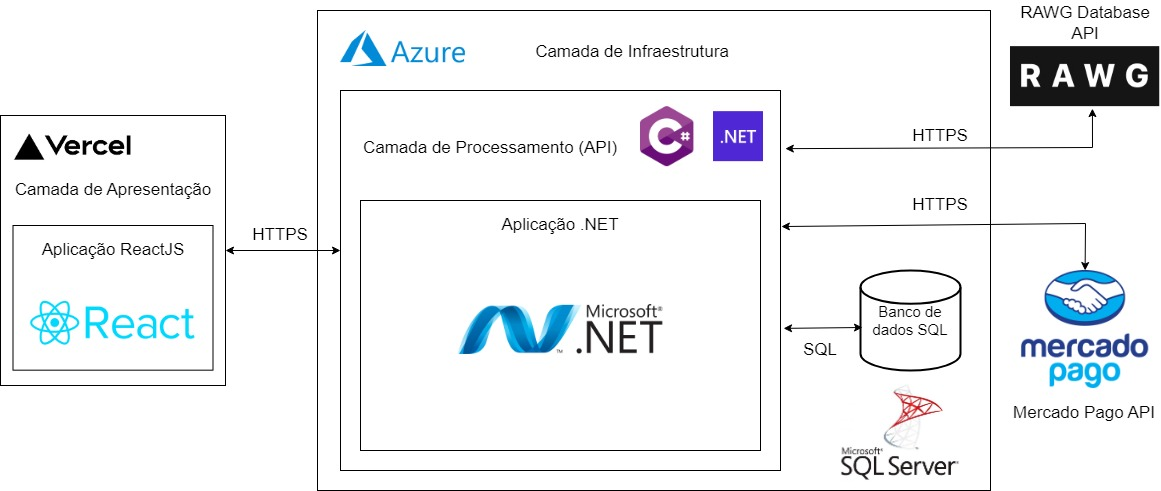
\includegraphics[scale = 0.37]{imagens/arquitetura/desenho_arquitetura.jpg}	
    \fonte{Os Autores}
\end{figure}

% Tecnologias e Ferramentas
\subsection{Tecnologias}

Nesta seção, apresentar-se-á uma visão geral de todas as tecnologias escolhidas para a implementação da aplicação, incluindo as linguagens de programação, \textit{\gls{Framework}} e bibliotecas utilizadas.

\subsubsection{Back-end}

No âmbito do \textit{\gls{Back-end}}, a escolha recaiu sobre a linguagem de programação \textit{\gls{Csharp}}, em concomitância com a plataforma de desenvolvimento e o \textit{Framework} \textit{\gls{.NET}}. Por conseguinte, foi concebida uma \ac{api} voltada ao gerenciamento da aplicação e à manipulação dos dados. No tocante à criação das tabelas do banco de dados e à gestão dos dados existentes, recorreu-se ao pacote \textit{\gls{Entity}}, que desempenha a função de \ac{orm} no âmbito deste projeto.

\subsubsection{Front-end}

No contexto do desenvolvimento do \textit{\gls{Front-end}} da aplicação, a linguagem de programação \textit{\gls{Javascript}} foi selecionada, em conjunto com a biblioteca \textit{\gls{React}}, para a construção dos componentes essenciais da plataforma. Adicionalmente, o \ac{css} foi empregado para conferir estilo às páginas, visando aprimorar a atratividade visual das interfaces aos olhos dos usuários. Por último, foram incorporadas bibliotecas destinadas a animação e ao controle de formulários, com o propósito de proporcionar suporte e otimizar a condução do processo de desenvolvimento da aplicação.

\subsubsection{Banco de dados}

Para a gestão e acesso aos dados, a opção recaiu sobre o \textit{\gls{Sqlserver}}, utilizando uma instância fornecida pelo serviço Azure. No processo de estruturação das tabelas e aplicação das etapas de normalização, a escolha foi direcionada à utilização do pacote \textit{\gls{Entity}}, desenvolvido pela \textit{\gls{Microsoft}}.

\subsubsection{Infraestrutura}

Quanto ao processo de \textit{\gls{Deploy}} da aplicação, é importante ressaltar que o \textit{\gls{Front-end}} foi devidamente hospedado na plataforma \textit{\gls{Vercel}}, enquanto o \textit{\gls{Back-end}} na plataforma da \textit{\gls{Azure}}.

\subsubsection{Escalabilidade}

As ferramentas disponibilizadas pela plataforma \textit{\gls{Azure}} foram empregadas no decorrer deste projeto, notadamente o sistema de dimensionamento automático. Tal emprego teve por objetivo primordial a adequação dinâmica da aplicação, alinhando-a de maneira precisa às demandas e necessidades apresentadas.

\subsubsection{APIs Externas}
Foram utilizadas duas \ac{api} externas para fornecer recursos e ferramentas à aplicação, sendo uma pertencente à \textit{\gls{Rawg}} e a outra, ao \gls{MercadoPago}.

A \ac{api} da \textit{\gls{Rawg}} foi utilizada por fornecer um
vasto conjunto de informações pertinentes ao universo dos jogos digitais, abrangendo
aspectos como o ano de lançamento, o estúdio desenvolvedor, os criadores e outros detalhes
relevantes.

Já a \ac{api} do \gls{MercadoPago} foi empregada para fornecer apoio ao fluxo de pagamento do plano premium fornecido pela aplicação, já que ela traz consigo todos os recursos necessários para realizar essas transações de forma segura.

% Critérios de Segurança/Privacidade/Legislação
\section{Critérios de Segurança/Privacidade/Legislação}
Esta seção tem como objetivo descrever, em termos gerais, os elementos de segurança implementados no projeto, bem como os critérios de privacidade seguidos e uma visão geral sobre seu enquadramento nos requisitos da \ac{lgpd}.

\subsection{Segurança Implantada para API Externa}

A obtenção de acesso à API da \textit{\gls{Rawg}} demanda a alocação de um domínio de site associado e, por este motivo, o domínio da \textit{GameLocker} foi estabelecido para esse propósito específico. Adicionalmente, como parte desse processo, foi criada uma chave de autenticação, a qual é necessária para ser inclusa em todas as requisições direcionadas à \ac{api}.

Nesse contexto, surge a necessidade de garantir a segurança da chave de autenticação. Tradicionalmente, as requisições à \ac{api} externa são efetuadas a partir do \textit{\gls{Front-end}} do projeto. No entanto, na presente situação, devido à sensibilidade da chave de autenticação, medidas adicionais se tornaram essenciais. Permitir que qualquer usuário do site a obtenha ao realizar requisições à \textit{GameLocker} seria um risco considerável.

Portanto, com a segurança em destaque, a decisão unânime foi a de implementar as requisições à \ac{api} da \textit{\gls{Rawg}} por meio do \textit{\gls{Back-end}}. Esse enfoque se revelou crucial para salvaguardar a chave de autenticação. Ao adotar essa abordagem, a chave não fica exposta às requisições realizadas pelos usuários no site, mitigando a possibilidade de utilização maliciosa. Em síntese, essa estratégia se alinha com as melhores práticas de segurança, garantindo a integridade e a confidencialidade da chave de autenticação, assim como a proteção do projeto em relação a potenciais atividades maliciosas.

\subsection{Segurança no Back-end}

Toda aplicação que almeja conquistar uma posição no mercado atual deve imperativamente oferecer uma camada de segurança robusta, com ênfase na autorização e autenticação de usuários. Nesse contexto, é fundamental reiterar que a autenticação consiste na validação da identidade de um usuário, assegurando a correspondência entre a alegação de identidade e a real identificação. Paralelamente, a autorização se refere aos recursos específicos que um usuário autenticado está habilitado a acessar.

Na \ac{api} concebida com a utilização da tecnologia \textit{\gls{.NET}}, optou-se por integrar o pacote \textit{\gls{Identity}}, desenvolvido e mantido pela \textit{\gls{Microsoft}}. O \textit{\gls{Identity}} oferece uma ampla gama de funcionalidades que simplificam a incorporação e o uso de sistemas de autenticação e autorização no contexto da aplicação. O primeiro aspecto de segurança abordado no âmbito do \textit{\gls{Back-end}} está relacionado ao procedimento de cadastro de usuários, o qual contempla diversas dimensões cruciais em termos de segurança.

Um exemplo notável é a exigência de que a senha atenda a critérios predefinidos, garantindo a solidez do registro do usuário na plataforma. Uma vez concluído o cadastro, o usuário é conduzido ao processo de autenticação no sistema, utilizando suas credenciais de e-mail e senha. É relevante destacar que os endereços de e-mail são exclusivos no ambiente da aplicação, sendo que a efetivação do login somente é possível mediante o fornecimento das credenciais precisas.

Com o êxito na autenticação, o sistema gera um componente de importância ímpar para o \textit{\gls{Front-end}} do projeto, denominado \textit{token} de autenticação do usuário. Visando assegurar uma proteção amplificada da aplicação, o acesso a qualquer recurso na \ac{api} do projeto requer a submissão do \textit{token} correspondente ao usuário. Tal \textit{token} é então validado no âmbito do \textit{\gls{Back-end}} do sistema, garantindo a integridade do processo de autorização e a salvaguarda dos recursos acessados.

\subsection{Segurança no Front-End}

No âmbito do desenvolvimento da aplicação, a segurança referente ao \textit{\gls{Front-end}} foi abordada com seriedade e profissionalismo, sendo implementadas uma série de medidas para salvaguardar informações pessoais e preservar a integridade das contas dos usuários. A seguir, são apresentadas algumas das principais ações de segurança adotadas:

\begin{itemize}
    \item Autenticação Convencional: Foi adotado um sistema de cadastro e login convencional para autenticar os usuários. Tal abordagem exige que cada usuário crie uma conta exclusiva com um nome de usuário e senha. As senhas são armazenadas de maneira criptografada no banco de dados, o que previne acessos não autorizados, garantindo a proteção da informação;
\end{itemize}

\begin{itemize}
    \item Certificado \ac{ssl}: A aplicação incorpora um certificado \ac{ssl} para estabelecer uma conexão segura entre o navegador do usuário e o servidor. Essa camada adicional de segurança cifra as informações transmitidas, incluindo dados pessoais e credenciais de login, para impedir qualquer tentativa de interceptação por terceiros mal-intencionados. A utilização do \ac{ssl} promove a confidencialidade e a integridade dos dados durante a interação entre o usuário e o servidor;
\end{itemize}

\begin{itemize}
    \item Protocolo \ac{https}: O protocolo \ac{https} foi adotado para todas as transações efetuadas no site. O \ac{https} é uma variante segura do protocolo \ac{http}, e sua presença indica que a comunicação entre o navegador do usuário e o servidor está protegida por criptografia. Esse enfoque resguarda as informações em trânsito, impedindo qualquer interceptação ou manipulação indesejada.
\end{itemize}

Adicionalmente a essas iniciativas, foram implementadas outras práticas de segurança recomendadas, incluindo atualizações regulares do software tanto do site quanto do servidor. Além disso, um sistema de monitoramento para detectar atividades suspeitas foi estabelecido, aprimorando a proteção e a vigilância contínua do ambiente digital.

\subsection{Segurança nos Repositórios}

O projeto é constituído por dois repositórios, nos quais os códigos do projeto são alocados e conservados. Enquanto um destes repositórios acolhe o código do \textit{\gls{Back-end}}, o outro desempenha a função de custodiar o código do \textit{\gls{Front-end}}. Com a finalidade de salvaguardar a integridade desses repositórios, eles são configurados como privados, uma medida que atua como uma barreira eficaz contra acessos, visualizações ou modificações por parte de indivíduos externos. Destarte, somente os membros integrantes do projeto ostentam a prerrogativa de autorização para adentrar e utilizar os recursos embutidos nesses repositórios.

\subsection{Segurança no Azure}

O processo de \textit{\gls{Deploy}} do projeto é executado através da plataforma de computação em nuvem da \textit{\gls{Azure}}. A própria plataforma \textit{\gls{Azure}} disponibiliza uma série de recursos dedicados à segurança para seus usuários, e esses recursos são integralmente empregados no âmbito deste projeto.

O primeiro recurso destaca-se por assegurar a proteção do acesso aos serviços hospedados na nuvem. Essa salvaguarda é estabelecida ao restringir o acesso somente a pontos críticos e essenciais, consolidando assim a salvaguarda dos serviços associados ao projeto.

Adicionalmente, uma segunda medida de segurança é aplicada através da limitação do \textit{\gls{Deploy}} do projeto na plataforma \textit{\gls{Azure}} exclusivamente para as máquinas que pertencem aos membros participantes do projeto. Essa estratégia contribui para acrescentar uma camada adicional de proteção ao processo de \textit{\gls{Deploy}}, mitigando potenciais riscos ao controlar estritamente o escopo das máquinas autorizadas a realizar o \textit{\gls{Deploy}} na plataforma.

\subsection{Lei Geral de Proteção de Dados}
A \ac{lgpd}, de acordo com o Congresso Nacional, "(...) dispõe sobre o tratamento de dados pessoais, inclusive nos meios digitais, por pessoa natural ou por pessoa jurídica de direito público ou privado, com o objetivo de proteger os direitos fundamentais de liberdade e de privacidade e o livre desenvolvimento da personalidade da pessoa natural." \cite{lgpd}.

Portanto, durante o desenvolvimento do projeto, foram tomadas decisões e
medidas de segurança para que ele se encaixasse e estivesse em conformidade com essa legislação, tendo foco em uma experiência segura para os usuários.

Os dados pessoais coletados para o cadastro, que são: nome completo, \textit{email}, telefone e data de nascimento, não se enquadram como dados pessoais sensíveis segundo o Art. 5°, II da \ac{lgpd} e, por este motivo, grande parte das restrições legislativas impostas não afetam diretamente o projeto.

Além disso, a aplicação permite o acesso aos dados pessoais fornecidos, bem como sua alteração, enquadrando-se no princípio de boa-fé do livre acesso aos dados, definido no Art. 6°,IV. A aplicação requisitará consentimento dos usuários para armazenar os dados fornecidos e manipulá-los como necessário para o funcionamento do sistema, o que confere a ela conformidade com o Art. 7°,I e Art. 6°,I.

Nos apêndices deste documento, no capítulo \ref{termos-e-condicoes}, estão detalhados os termos e condições com os quais o usuário precisará concordar para utilizar a aplicação.

% Documentação da API (Swagger)
\section{Documentação}

Uma documentação bem elaborada proporciona inúmeros benefícios para o desenvolvimento de projetos na área da tecnologia. No caso da \ac{api} desenvolvida em \textit{\gls{.NET}}, a documentação das suas rotas de acesso foi realizada por meio do \textit{\gls{Swagger}}, com o objetivo de facilitar o entendimento de cada rota e sua função no sistema.

A imagem inaugural aborda de maneira específica as rotas correspondentes aos mecanismos de acesso e ao gerenciamento da conta do usuário. Estes \textit{\gls{Endpoints}} podem ser observados com clareza na Figura \ref{RotasAccount}, sendo que cada um é acompanhado por uma exposição elucidativa acerca do propósito subjacente de sua funcionalidade.

\begin{figure}[H]
    \centering
	\caption{Rotas do Usuário}
    \label{RotasAccount}
    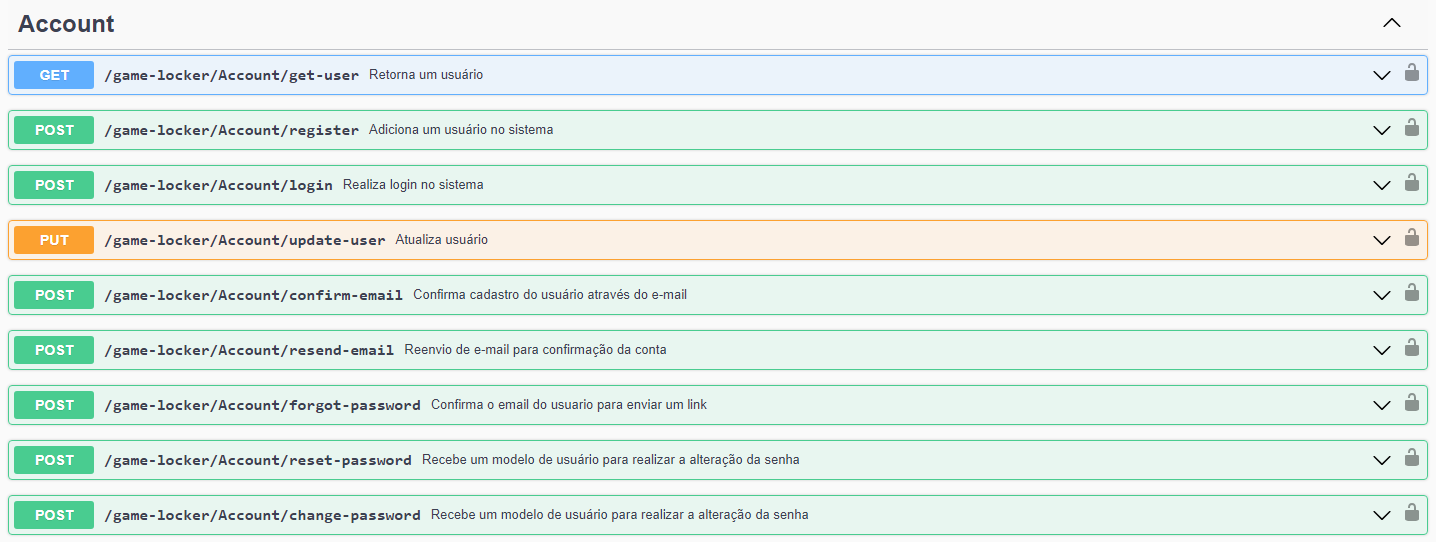
\includegraphics[scale = 0.38]{imagens/arquitetura/rotas_account.png}	
    \fonte{Os Autores}
\end{figure}

A segunda representação gráfica ilustra de maneira distintiva a rota destinada ao acesso a uma \ac{api} externa fornecida pela \textit{\gls{Rawg}}. É imperativo enfatizar que esta invocação à \ac{api} externa ocorre de modo exclusivo no \textit{\gls{Back-end}}, uma precaução tomada em virtude das considerações de segurança inerentes à aplicação. A Figura \ref{RotasApi} proporciona uma visualização precisa dessa rota singular, oferecendo uma compreensão nítida do seu papel e relevância intrínseca no contexto da arquitetura da aplicação.

\begin{figure}[H]
    \centering
	\caption{Rota da API externa}
    \label{RotasApi}
    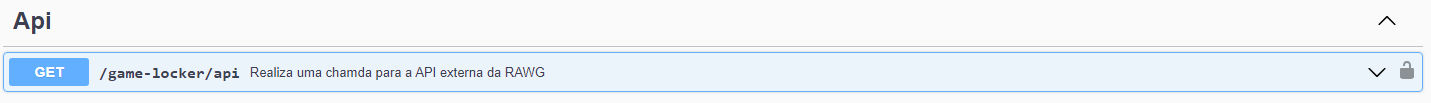
\includegraphics[scale = 0.38]{imagens/arquitetura/rotas_api.png}	
    \fonte{Os Autores}
\end{figure}

A terceira representação gráfica fornece uma visão abrangente de todas as rotas relacionadas às \gls{Review} no âmbito da aplicação. Esta seção assume um papel central na aplicação, demandando, assim, uma ênfase adicional em termos de considerações. A Figura \ref{RotasReview} elucida essas rotas de maneira detalhada, delineando as respectivas funcionalidades que desempenham no contexto do projeto.

\begin{figure}[H]
    \centering
	\caption{Rotas de Review}
    \label{RotasReview}
    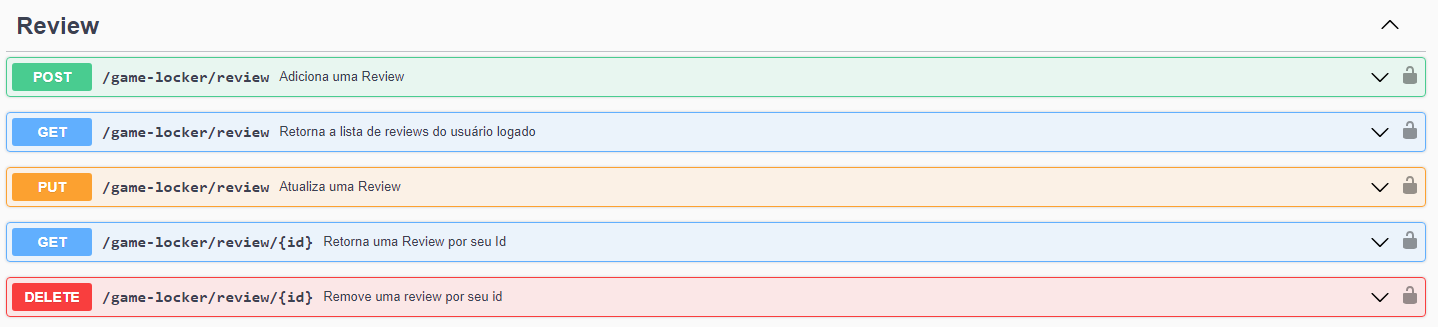
\includegraphics[scale = 0.38]{imagens/arquitetura/rotas_review.png}	
    \fonte{Os Autores}
\end{figure}

A figura \ref{RotasArena} descreve as rotas relacionadas à Arena de Jogos da Aplicação, fornecendo um panorama geral sobre as responsabilidades dessas rotas.

\begin{figure}[H]
    \centering
	\caption{Rotas de Arena}
    \label{RotasArena}
    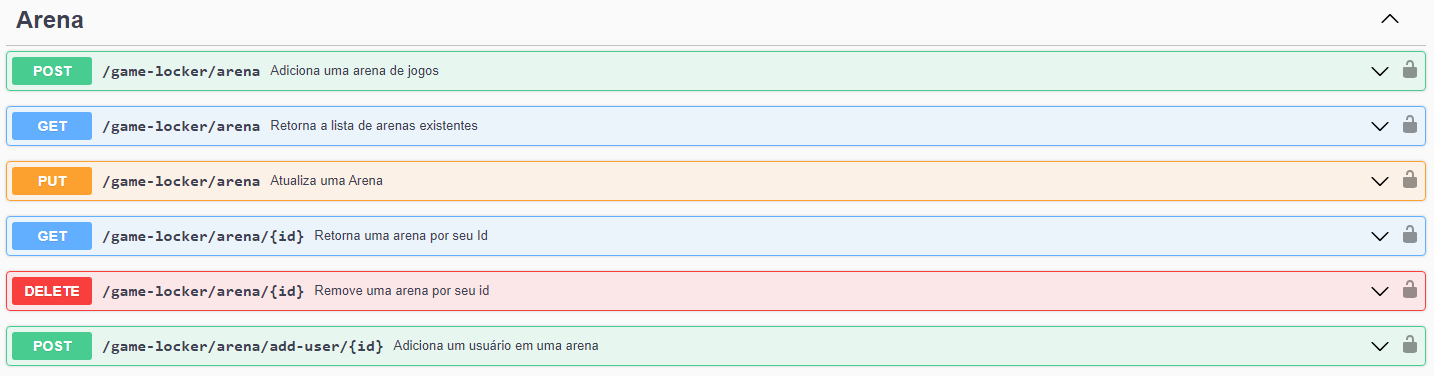
\includegraphics[scale = 0.38]{imagens/arquitetura/rotas_arena.png}	
    \fonte{Os Autores}
\end{figure}

Na figura \ref{RotasPayment} descreve as rotas que interagem diretamente com a \ac{api} do \gls{MercadoPago}, permitindo que as transações sejam realizadas de maneira segura no momento de adesão ao plano premium fornecido na plataforma.

\begin{figure}[H]
    \centering
	\caption{Rotas de Pagamento e Assinaturas}
    \label{RotasPayment}
    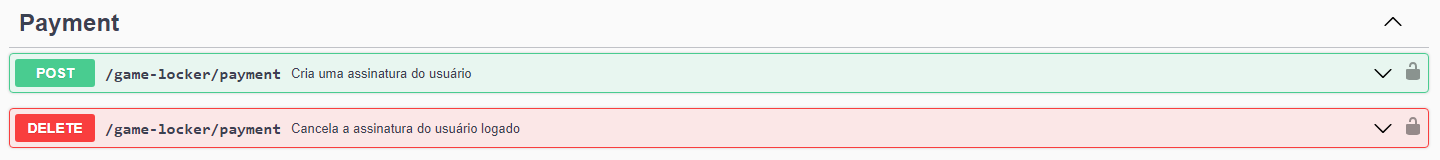
\includegraphics[scale = 0.38]{imagens/arquitetura/rotas_payment.png}	
    \fonte{Os Autores}
\end{figure}

Na Figura \ref{AutenticacaoSwagger}, encontra-se a representação da seção do \gls{Swagger} que assume a responsabilidade pela implementação da autenticação na presente \ac{api}. Importante ressaltar que todas as rotas pertencentes ao \textit{\gls{Back-end}} do projeto, com exceção das rotas de login e cadastro de contas, impõem a necessidade de autenticação para possibilitar o acesso.

\begin{figure}[H]
    \centering
	\caption{Autenticação do Swagger}
    \label{AutenticacaoSwagger}
    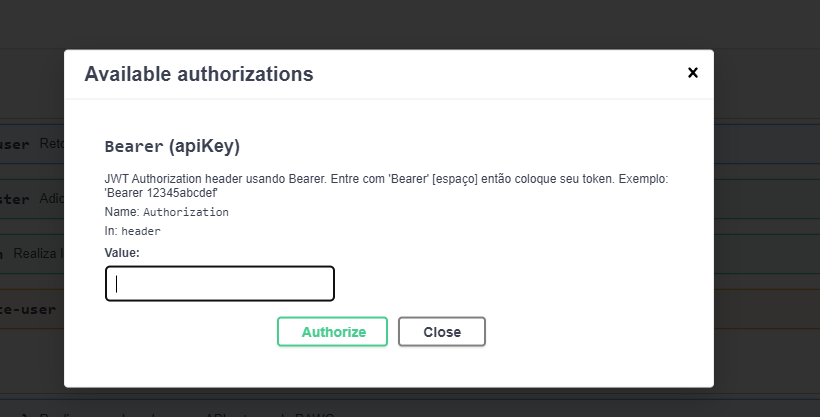
\includegraphics[scale = 0.6]{imagens/arquitetura/rotas_token.png}	
    \fonte{Os Autores}
\end{figure}

Por derradeiro, na Figura \ref{ObjetosEndpoints}, são exibidos em detalhe todos os objetos inerentes às rotas do sistema. Estes objetos carregam a responsabilidade primordial de armazenar e veicular os dados através das interações na aplicação.

\begin{figure}[H]
    \centering
	\caption{Objetos dos Endpoints}
    \label{ObjetosEndpoints}
    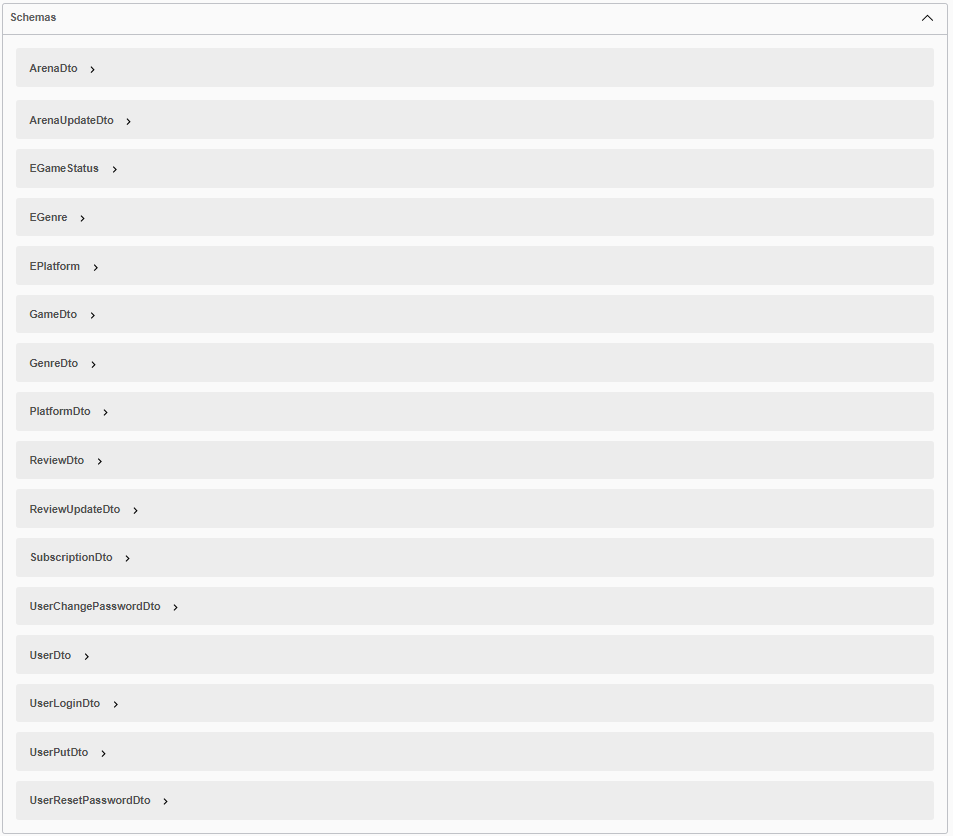
\includegraphics[scale = 0.6]{imagens/arquitetura/rotas_schemas.png}	
    \fonte{Os Autores}
\end{figure}

Para mais informações sobre a \ac{api} do projeto, consultar o link presente no capítulo \ref{LinksProjeto}, que contém este e outros links relevantes.

% Fases de Entrega
\clearpage
\section{Fases de Entrega}

Nesta seção, são estabelecidas as datas cruciais e as fases significativas do desenvolvimento do projeto, nas quais ocorrerão as entregas progressivas e escalonadas.

\subsection{Desenho da Aplicação}

No Desenho da Aplicação, foram disponibilizadas as informações essenciais para proporcionar uma compreensão abrangente tanto do projeto em si quanto da aplicação em sua totalidade. Essa entrega englobou elementos como a arquitetura, os objetivos estabelecidos e os métodos empregados no processo de desenvolvimento. O momento dessa entrega se deu no mês de abril de 2023.

\subsection{Prova de Conceito}

Na \ac{poc}, foram executadas as ações essenciais para evidenciar o funcionamento do sistema. Isso abrangeu a interligação da \ac{api} elaborada em linguagem \textit{\gls{Csharp}} e a construção da interface \textit{\gls{Front-end}} empregando a tecnologia \textit{\gls{React}}. Paralelamente, ocorreu a integração harmoniosa do sistema com a \ac{api} externa da \textit{\gls{Rawg}} e a subsequente realização do processo de implantação na plataforma \textit{\gls{Azure}}. A conclusão desta etapa ocorreu no mês de maio de 2023.

\subsection{Produto Mínimo Viável}

No \ac{mvp}, foram disponibilizadas as funcionalidades primordiais do projeto. Isso compreendeu a implementação da criação de contas e usuários, o sistema de login, bem como a validação de credenciais e identidades dos usuários. Foi igualmente elaborada uma \textit{\gls{LandingPage}} voltada para a visualização de usuários não autenticados. Além disso, um portal foi estabelecido para abarcar todos os jogos disponíveis, com funcionalidades para avaliação e observação. Destaca-se ainda a incorporação de filtros à lista de jogos, a criação de perfis de usuários e a capacidade de gerenciar jogos de forma individualizada para cada usuário. 

Este marco foi atingido no mês de junho de 2023, consolidando a entrega das bases funcionais do sistema.

\subsection{Produto}

No Produto, a entrega englobará a versão completa do projeto, abarcando integralmente todas as funcionalidades planejadas. Dentro desse rol de funcionalidades, merece destaque o desenvolvimento do sistema de arenas de jogos, a criação de chats dedicados, e a implementação da capacidade de visualizar perfis de outros usuários.

Adicionalmente, o projeto compreenderá a configuração do ciclo completo para a realização de assinaturas na aplicação, abarcando tanto a alternativa de assinatura \textit{premium} quanto a disponibilização de anúncios para os usuários comuns. A expectativa é que essa versão final seja entregue até o mês de dezembro de 2023, consolidando assim a realização plena das metas e objetivos traçados para o desenvolvimento do sistema.

% Historia de Usuario
\section{Histórias de usuário}

\begin{enumerate}
  \item \textbf{Cadastro}
  
  \textbf{Caso:} Eu, como jogador de jogos digitais, quero realizar o cadastro no site \textit{GameLocker} para fazer o gerenciamento de meus jogos e conhecer a comunidade de \textit{players}.
  
  \textbf{Critérios de Aceitação:}
  \begin{itemize}
      \item O usuário deve conseguir fazer o cadastro;
      \item O usuário deve possuir no mínimo 16 anos;
      \item E-mail do usuário deve ser único no sistema;
      \item Username do usuário deve ser único no sistema;
      \item A senha deve seguir os padrões necessários do site.
  \end{itemize}
  
  \item \textbf{Login}

  \textbf{Caso:} Eu, como jogador de jogos digitais, quero realizar o login no site GameLocker para fazer o gerenciamento de meus jogos e conhecer a comunidade de \textit{players}.
  
  \textbf{Critérios de Aceitação:}
  \begin{itemize}
      \item O usuário deve conseguir fazer o login;
      \item O usuário deve fornecer e-mail e senha corretos;
      \item O usuário não deve conseguir acessar os recursos sem estar logado;
      \item O usuário não deve conseguir fazer login com credenciais erradas.
  \end{itemize}
  
   
  \item \textbf{Adicionar Jogo/Review}

  \textbf{Caso:} Eu, como jogador de jogos digitais, quero poder adicionar a review de um jogo que estou jogando, além de oferecer uma nota e comentários para esse jogo.

  \textbf{Critérios de Aceitação:}
  \begin{itemize}
      \item O usuário deve conseguir adicionar uma review;
      \item O usuário deve conseguir colocar uma nota e um comentário para o jogo escolhido;
      \item O usuário deve selecionar um status para o jogo, o padrão deve ser jogando;
      \item O jogo adicionado pelo usuário deve ir para seu perfil.
  \end{itemize}

  \item \textbf{Visualizar reviews}

  \textbf{Caso:} Eu, como usuário que fiz reviews, quero visualizar todas minhas reviews feitas em meu perfil, para poder gerenciar elas de forma objetiva.

  \textbf{Critérios de Aceitação:}
  \begin{itemize}
      \item O usuário deve conseguir visualizar todas suas reviews;
      \item O usuário deve conseguir filtras as reviews por abas relacionadas a seus status.
  \end{itemize}

  \item \textbf{Editar Review}

  \textbf{Caso:} Eu, como usuário que adicionei uma review, quero ter a chance de editar os dados dela.

  \textbf{Critérios de Aceitação:}
  \begin{itemize}
      \item O usuário deve conseguir clicar na review escolhida e abrir um modal para editar a review;
      \item O usuário deve conseguir editar os campos liberados da review;
      \item As edições não devem ser persistidas caso o usuário não clique em salvar;
      \item Ao clicar em salvar, as edições devem ser persistidas, uma mensagem de sucesso deve aparecer e o usuário deve ser redirecionado para a listagem.
  \end{itemize}

  \item \textbf{Remover Review}

  \textbf{Caso:} Eu, como usuário que adicionei uma review errada, quero poder remover ela de forma fácil e rápida.

  \textbf{Critérios de Aceitação:}
  \begin{itemize}
      \item Ao clicar em remover, a review deve ser removida do banco de dados;
      \item Ao fazer a remoção, usuário deve ser redirecionado para a listagem atualizada.
  \end{itemize}

  \item \textbf{Filtrar Jogos Adicionados}

  \textbf{Caso:} Eu, como usuário possuo vários jogos adicionados, quero filtrar eles por nome do jogo.

  \textbf{Critérios de Aceitação:}
  \begin{itemize}
      \item Deve ter na tela uma barra de pesquisa para digitação do usuário;
      \item Filtragem deve ocorrer enquanto o usuário escreve, de forma a aparecer os resultados atualizados;
      \item Deve ter um ícone de apagar para caso o usuário queira remover o texto digitado;
      \item Ao remover o texto digitado, a listagem deve voltar ao normal;
      \item Caso não possua nenhuma correspondência para o texto digitado, deve aparecer uma mensagem informativa.
  \end{itemize}

  \item \textbf{Criar arena de jogos}

   \textbf{Caso:} Eu, como usuário premium, quero criar uma arena de um jogo para fazer um torneio entre jogadores.

   \textbf{Critérios de Aceitação:}
  \begin{itemize}
      \item Somente usuários premium podem criar arena;
      \item O administrador precisar definir algumas configurações obrigatórias no momento de criação de arena;
  \end{itemize}

  \item \textbf{Entrar na arena de jogos}

   \textbf{Caso:} Eu, como usuário que estou procurando amigos para jogar, quero entrar numa arena de algum jogo.

   \textbf{Critérios de Aceitação:}
  \begin{itemize}
      \item Deve ter a listagem de arenas disponíveis;
  \end{itemize}
  
\end{enumerate}

% Manutenibilidade
\clearpage
\section{Manutenibilidade}

Com o objetivo de garantir a longevidade da aplicação e facilitar a implementação de novas funcionalidades, torna-se crucial que a equipe de desenvolvimento siga padrões, princípios e boas práticas estabelecidos. Adicionalmente, é importante mencionar que a implementação de boas práticas não se limita apenas à codificação, mas se estende também à documentação, comunicação e colaboração entre os membros da equipe.

\subsection{Ferramentas para Testes automatizados e Análise Estática}

Para a realização dos testes automatizados no \textit{\gls{Back-end}}, será utilizado o \textit{\gls{Xunit}}, uma ferramenta de código aberto empregada para a execução de testes automatizados. Essa ferramenta oferece recursos avançados, como a paralelização de testes e a capacidade de executá-los em diversas plataformas. Além disso, o \textit{\gls{Xunit}} possui uma documentação abrangente e integração com a \ac{IDE} do \textit{\gls{VisualStudio}}, que será utilizada no desenvolvimento.

\subsection{Code Convention}

Para o desenvolvimento do \textit{\gls{Back-end}}, adotou-se a convenção de codificação da linguagem \textit{\gls{Csharp}}, conhecida como \textit{Csharp Coding Conventions}. Essa convenção foi criada e é mantida pela \textit{\gls{Microsoft}}, empresa responsável pela criação da linguagem de programação \textit{\gls{Csharp}}. É possível encontrar a documentação completa dessa convenção online. Entre as principais definições dessa convenção, destacam-se:

\begin{itemize}
\item Nomes de variáveis devem ser descritivos, utilizando-se sempre \texttt{\gls{CamelCase}} (inicia com letra minúscula);
\item Nomes de classes e tipos devem ser descritivos, iniciando com letra maiúscula e utilizando \texttt{\gls{PascalCase}};
\item Métodos devem ser nomeados utilizando verbos, seguidos de um substantivo ou frase descritiva;
\item Utilize indentação de 4 espaços, sem tabulação;
\item Chaves devem ser abertas na mesma linha que o código que as precede e fechadas em uma nova linha;
\item Cada instrução deve ser escrita em uma linha separada;
\item A largura da linha não deve ultrapassar 120 caracteres;
\item Utilize comentários em linha para explicar partes do código que possam ser difíceis de entender;
\item Use espaços em branco para separar operadores e elementos do código;
\item Utilize a palavra-chave \textit{\texttt{this}} para referenciar membros da classe atual.
\end{itemize}

Para o desenvolvimento do \textit{\gls{Front-end}}, foi utilizado o \textit{Google TypeScript Style Guide}, que é um guia de estilo de codificação para o \textit{\gls{Typescript}}, uma linguagem de programação desenvolvida pela \textit{\gls{Microsoft}}. Esse guia é mantido pelo \textit{Google} e fornece diretrizes para padronizar a escrita de código em projetos que utilizam \textit{\gls{Typescript}}.

Algumas das principais características desse guia são:

\begin{itemize}
\item Uso de \texttt{\gls{CamelCase}} para nomes de variáveis e \texttt{\gls{PascalCase}} para nomes de tipos e classes;
\item Uso de \textit{\texttt{const}} em vez de \textit{\texttt{let}} sempre que possível;
\item Uso de tipos explícitos em vez de inferência de tipos sempre que possível;
\item Evitar o uso de tipos \textit{\texttt{any}} sempre que possível;
\item Uso de \texttt{===} em vez de \texttt{==} para comparações;
\item Evitar o uso de \textit{\texttt{namespace}} e, em vez disso, utilizar módulos;
\item Uso de \texttt{interface} para definição de tipos e estruturas de objetos;
\item Utilização de apóstrofo para strings;
\item Uso de \textit{arrow functions} em vez de function expressions sempre que possível;
\item Uso de \textit{\texttt{async/await}} em vez de \textit{callbacks} para operações assíncronas.
\end{itemize}

\subsection{Integração Continua}

O \ac{ci}/\ac{cd} do GitHub é uma ferramenta amplamente utilizada em projetos de software em todo o mundo, sendo uma opção confiável e robusta para a implementação de processos de \ac{ci}/\ac{cd}. Com sua flexibilidade e facilidade de configuração, é possível acelerar a entrega de software com qualidade e eficiência.

Dentre os processos que podem ser integrados na integração contínua com o \ac{ci}/\ac{cd} do GitHub, encontram-se a restauração/instalação de dependências, a compilação, a execução de testes automatizados e a geração de artefatos para implantação. Essa integração permite garantir a qualidade do código e reduzir o tempo de entrega de novas funcionalidades.

A aplicação do \ac{ci}/\ac{cd} do GitHub no projeto será realizada através da configuração de um servidor de integração contínua, com o objetivo de automatizar o processo de \textit{build} e testes. A cada \textit{commit} efetuado por um membro da equipe em sua respectiva \textit{branch}, o \ac{ci}/\ac{cd} do GitHub assumirá automaticamente a responsabilidade de realizar o \textit{build} do código e executar os testes automatizados.

\subsection{Design Patterns e Princípios de Design de Software}

No desenvolvimento do \textit{\gls{Front-end}} e do \textit{\gls{Back-end}}, foram seguidos dois conjuntos de princípios e diretrizes de design de software: o \textit{\gls{CleanCode}} e o \textit{\gls{SOLID}}. O \textit{\gls{SOLID}} e o \textit{\gls{CleanCode}} são dois conceitos fundamentais no desenvolvimento de software orientado a objetos que têm como objetivo aprimorar a qualidade e a legibilidade do código. Ambos são de extrema importância, pois tornam o código mais fácil de compreender, modificar e manter ao longo do tempo.

Foram estritamente seguidas as orientações preconizadas pelo \textit{\gls{CleanCode}}, com o propósito de discernir setores passíveis de aprimoramento no código preexistente e inaugurar o processo de refatoração. O intento primordial reside na simplificação das funções de caráter intrincado, na atribuição de denominações mais expressivas às variáveis e na reconfiguração de segmentos enredados do código-fonte. O cerne desse empenho é alinhar o código com as práticas mais salutares de desenvolvimento, otimizando assim a legibilidade, a manutenibilidade e a compreensibilidade do sistema como um todo.

Foram diligentemente incorporados sólidos padrões de design, reconhecidos como os princípios \textit{\gls{SOLID}}, para estabelecer os alicerces essenciais na arquitetura deste projeto. Estes princípios fundados na orientação a objetos, abarcando os preceitos de \ac{srp}, \ac{ocp}, \ac{lsp}, \ac{isp} e \ac{dip}, foram criteriosamente adotados com a finalidade precípua de fomentar uma estrutura sólida e altamente flexível.

\subsubsection{Clean Code}

O \textit{\gls{CleanCode}} engloba um conjunto criterioso de orientações e práticas concebidas com a finalidade precípua de aprimorar a legibilidade, a compreensibilidade e a manutenibilidade do código de um software. Dentre as diretrizes preeminentes, evidenciam-se as seguintes:

\begin{itemize}
    \item Atribuição de denominações de cunho substancial a classes, métodos, propriedades e variáveis;
    \item Eliminação de redundâncias no código-fonte;
    \item Concepção de métodos breves, os quais ostentam uma única incumbência;
    \item Elaboração de código que é simultaneamente simples e de natureza acessível para compreensão.
\end{itemize}

\subsubsection{SOLID}

O acrônimo \textit{\gls{SOLID}}, que representa um conjunto de cinco princípios fundamentais para o desenvolvimento de software orientado a objetos, é amplamente reconhecido e empregado na indústria de tecnologia. Estes princípios e diretrizes têm como objetivo central a criação de código-fonte de software caracterizado por sua modularidade, flexibilidade e facilidade de manutenção.

Tais princípios desempenham um papel crucial ao auxiliar os desenvolvedores na elaboração de sistemas que apresentam não apenas flexibilidade e escalabilidade, mas também facilidade de manutenção. Através da promoção da coesão entre os componentes e da minimização do acoplamento indesejado, esses princípios fornecem orientações valiosas para a construção de sistemas de software robustos e sustentáveis.

% Modelo Entidade Relacionamento (MER)
\clearpage
\section{Modelo Entidade Relacionamento (MER)}
A figura \ref{DiagramaMer} busca descrever as entidades no domínio de negócios do projeto, com foco no entendimento de seus relacionamentos de forma mais ampla.

% \begin{figure}[hb]
%     \centering
% 	\caption{Diagrama MER}
%     \label{DiagramaMer}
%     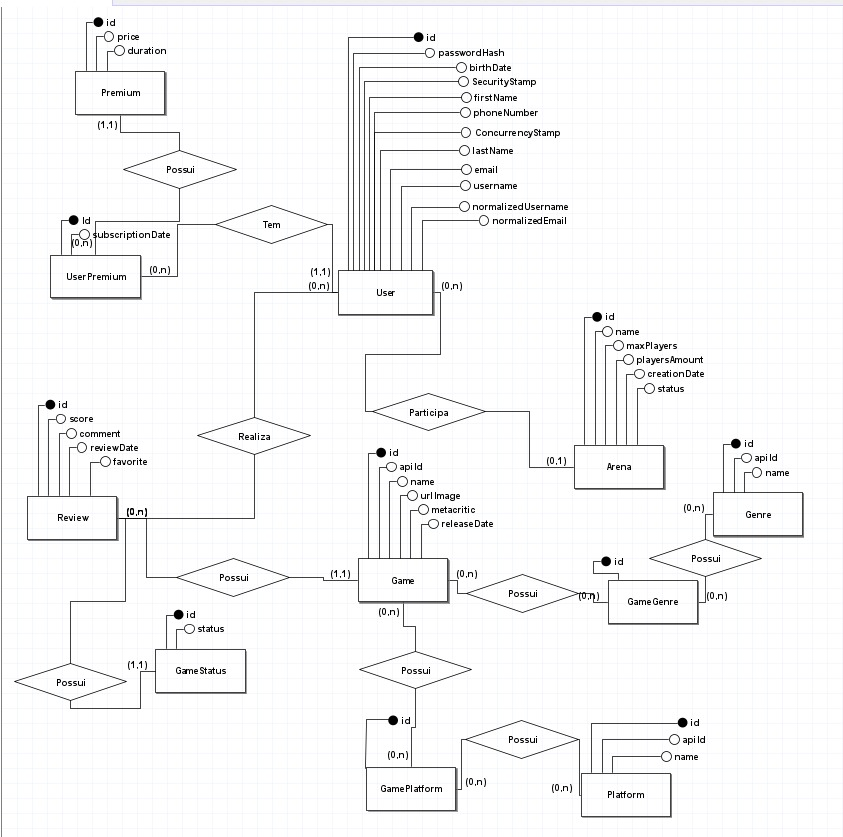
\includegraphics[scale = 0.50]{imagens/arquitetura/diagrama-mer.jpeg}	
%     \fonte{Os Autores}
% \end{figure}

\begin{sidewaysfigure}
    \centering
    \caption{Diagrama MER}
    \label{DiagramaMer}
    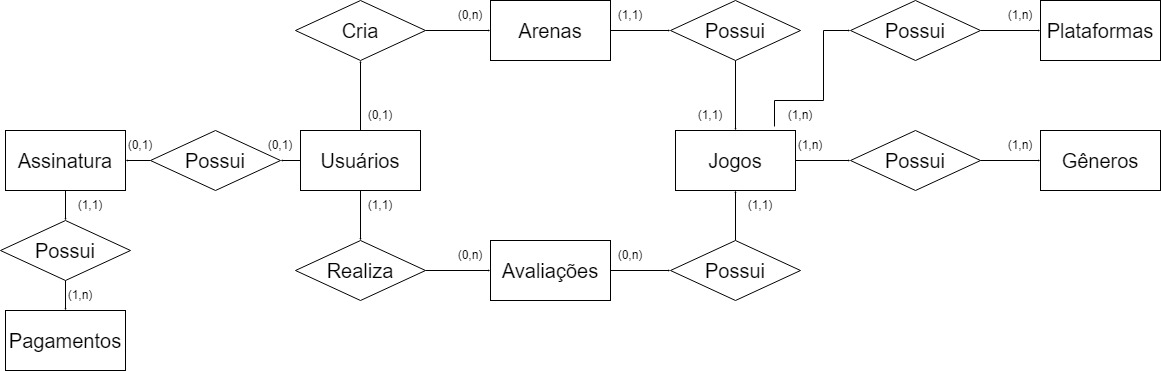
\includegraphics[scale=0.60]{imagens/arquitetura/diagrama-mer-new.jpg}
    \fonte{Os Autores}
\end{sidewaysfigure}

% Diagrama Entidade Relacionamento (DER)
\clearpage
\section{Diagrama Entidade Relacionamento (DER)}
A figura \ref{DiagramaDer} tem como objetivo representar com mais detalhes os atributos e relacionamentos das tabelas do banco de dados da aplicação.

\begin{sidewaysfigure}
    \centering
	\caption{Diagrama DER}
    \label{DiagramaDer}
    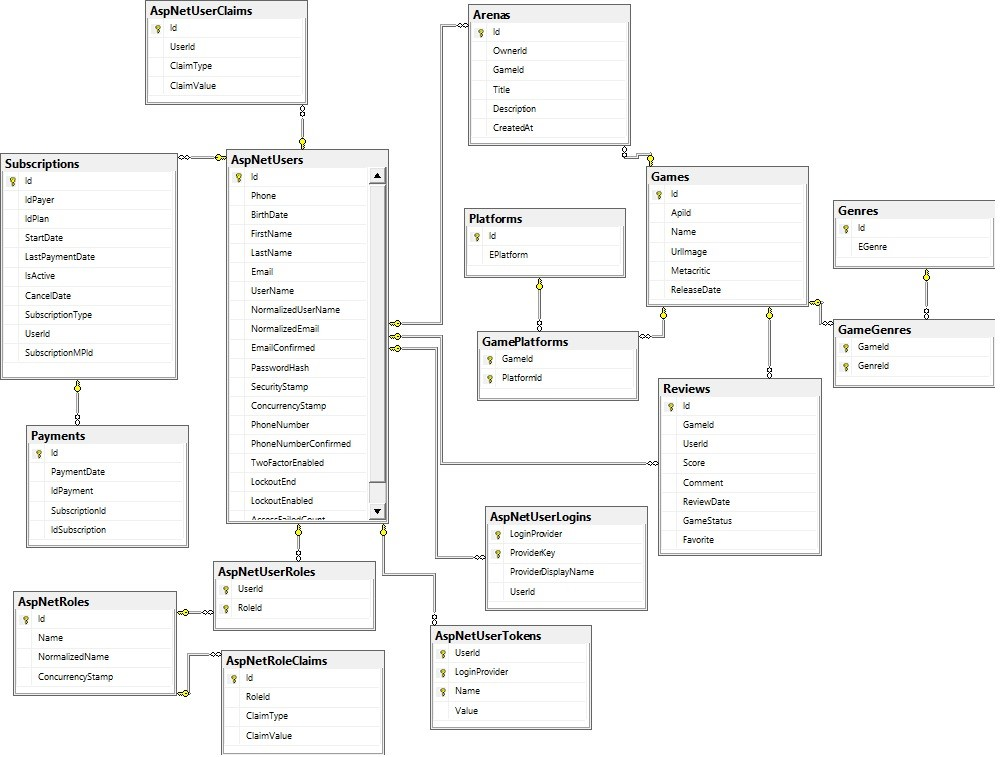
\includegraphics[scale =0.70]{imagens/arquitetura/diagrama-der.jpeg}	
    \fonte{Os Autores}
\end{sidewaysfigure}

% Volumetria
\clearpage
\section{Volumetria}

A volumetria configura-se como um conceito de relevância primordial no tocante à mensuração das dimensões e ao espaço apropriado que o repositório de dados de determinada aplicação ocupa. Além disso, reveste-se de caráter prospectivo ao possibilitar a estimativa da ocupação futura. Estas informações revestem-se de absoluta importância para a delineação adequada do projeto em si e do arcabouço informacional subjacente, o que ganha contornos ainda mais destacados em corporações de grande envergadura. Tal como pode ser constatado no Quadro \ref{volumetria}, o atual tamanho do banco de dados da aplicação \textit{GameLocker} é estimado em aproximadamente 16MB.

\begin{quadro}[thb]
\centering
\ABNTEXfontereduzida
\caption{Tamanho do Banco de Dados}

\begin{tabular}{|l|c|c|c|}
\hline
\thead{Name} & \thead{DB Size} \\
\hline
GameLockerdb & 16.00 MB \
\\\hline
GameLockerdb2 & 16.00 MB \
\\\hline
GameLockerdb3 & 16.00 MB \
\\\hline
\end{tabular}
\label{volumetria}
\fonte{Autores}
\end{quadro}


% Viabilidade Financeira
\chapter{Viabilidade financeira}

No âmbito do desenvolvimento de uma aplicação, a avaliação de sua viabilidade financeira assume um papel de extrema importância, exercendo influência significativa na análise de projetos e na formulação de decisões estratégicas. A primordialidade deste aspecto se funda na sua capacidade de assegurar uma avaliação meticulosa dos encargos associados e uma projeção pragmática das receitas projetadas, ambas essenciais para garantir a sustentabilidade do projeto e a concretização de um retorno financeiro condizente com os objetivos almejados.

% Estimativas
\section{Estimativas de usuários}

Esta seção tem como objetivo traçar uma estimativa dos possíveis usuários da plataforma desenvolvida, com o intuito de fornecer embasamento aos cálculos para realizar as previsões financeiras.

\subsection{Aplicações com público-alvo semelhantes}\label{subsec::publico-alvo_semelhante}

Neste tópico, serão analisadas as plataformas que possuem um público-alvo semelhante ao da \textit{GameLocker}. O objetivo da análise é alcançar um valor equilibrado para a assinatura \textit{premium} do sistema e realizar uma estimativa geral dos usuários que podem ser alcançados, levando em consideração a proporção de uma plataforma recém-lançada.

\subsubsection{Discord}

A plataforma \textit{\gls{Discord}} engloba chamadas de voz, mensagens escritas e uma gama variada de recursos para seus usuários. Conforme citado por Ash Turner \cite{discord_users}, aproximadamente 70\% dos usuários da plataforma a utilizam para jogar \textit{videogame} e outras atividades, como grupos de estudos. Essa informação leva à conclusão de que o público-alvo desse sistema se assemelha ao da \textit{GameLocker}.

De acordo com informações disponíveis no site oficial do \textit{\gls{Discord}} (Disponível em: \url{https://discord.com/nitro}), a plataforma oferece uma opção de assinatura mensal ao custo de \textit{R\$ 25,00}. Essa assinatura proporciona aos utilizadores a expansão da capacidade de \textit{uploads} de arquivos, uma personalização mais profunda de perfis, bem como a capacidade de transmitir vídeos em alta definição (HD), entre outros benefícios de significativa relevância.

\subsubsection{Twitch}

A \textit{\gls{Twitch}}, atualmente, desempenha um papel de destaque como uma das mais renomadas plataformas de transmissão em tempo real global. Conforme apontado pela VentureBeat \cite{twitch_categories}, nove das dez categorias mais assistidas na \textit{\gls{Twitch}} estão relacionadas a jogos eletrônicos, mantendo-se constantemente em evidência e atraindo diariamente centenas de milhares de espectadores. Essa dinâmica a torna um espaço amplamente explorado pelo público-alvo que este projeto busca alcançar.

De acordo com informações disponíveis em seu site oficial \url{https://www.twitch.tv}, a plataforma oferece uma opção de assinatura mensal com um custo de \textit{R\$ 26,99}. Através dessa assinatura, os usuários podem desfrutar da visualização de conteúdo livre de anúncios indesejados e têm acesso a um conjunto diversificado de recursos destinados à personalização de seus perfis. Isso inclui a utilização de \textit{emotes} personalizados, a variação de paletas de cores e a obtenção de distintivos especiais, contribuindo assim para uma experiência mais envolvente e individualizada.

\subsubsection{Estratégias de Utilização}

Este tópico visa investigar e analisar as estratégias que transformaram o \textit{\gls{Discord}} e o \textit{\gls{Twitch}} em líderes na arena da comunicação online, transcendo as suas origens como plataformas voltadas para jogos. Além disso, serão apresentadas estatísticas relacionadas ao uso e à receita dessas plataformas.

\subsubsubsection{Plano de Aplicação}

O \textit{\gls{Discord}}, desde a sua introdução em 2015, tem percorrido uma notável trajetória de evolução e adaptação, culminando na redefinição de sua imagem inicial, que estava originalmente vinculada a uma plataforma exclusivamente voltada para jogos.

\begin{itemize}
    \item \textbf{Diversificação de Servidores}: Servidores dedicados a jogos, permitindo que os jogadores se reunissem em um ambiente específico para cada jogo;
    \item \textbf{Expansão para Além dos Jogos}: Embora tenha começado como uma plataforma de jogos, o \textit{\gls{Discord}} expandiu sua base de usuários para incluir não jogadores, competindo com ferramentas de comunicação empresarial como \textit{Slack} e \textit{Microsoft Teams};
    \item \textbf{Combate à Controvérsia}: O \textit{\gls{Discord}} enfrentou desafios, incluindo a controvérsia em torno do uso de servidores privados por grupos extremistas. A empresa implementou ferramentas de moderação e verificação para lidar com esses problemas, destacando seu compromisso com a segurança e responsabilidade.
\end{itemize}

A \textit{\gls{Twitch}}, uma plataforma líder de comunicação, tem expandido significativamente seu escopo muito além de sua imagem inicial, que estava predominantemente associada à transmissão de jogos.

\begin{itemize}
    \item \textbf{Diversificação de Conteúdo}: Embora o \textit{\gls{Twitch}} seja amplamente associado à transmissão de jogos, a plataforma diversificou seu conteúdo ao longo do tempo. Além das transmissões de jogos, os criadores agora utilizam o \textit{Just Chatting} e outras categorias para transmitir uma variedade de conteúdos, como shows ao vivo, música e arte;
    \item \textbf{Parcerias e Integrações}: Estabelecer parcerias estratégicas com empresas e criadores de conteúdo, o que ajudou a atrair um público diversificado. Além disso, integrações com plataformas como \textit{\gls{Amazon Prime}} e eventos como o \textit{TwitchCon} fortaleceram a presença da plataforma;
    \item \textbf{Monetização para Criadores}: Introduzir maneiras inovadoras de monetização para criadores, como assinaturas de canais, doações e anúncios. Essas estratégias tornaram possível que criadores ganhassem renda significativa transmitindo seu conteúdo na plataforma.
\end{itemize}

\subsubsubsection{Estatísticas de Uso e Receita}

A \textit{\gls{Twitch}} registra 140 milhões de usuários ativos mensais, demonstrando sua extensa popularidade. Essa estatística por si só destaca a importância da plataforma no cenário de entretenimento online. Conforme apontado pela Backlink \cite{twitch_growth_statistics} e descrito na Figura \ref{crescimentoUsoTwitch}.

\begin{figure}[H]
    \center
	\caption{\label{fig_sge20}Crescimento do Uso da Twitch}
    \label{crescimentoUsoTwitch}
    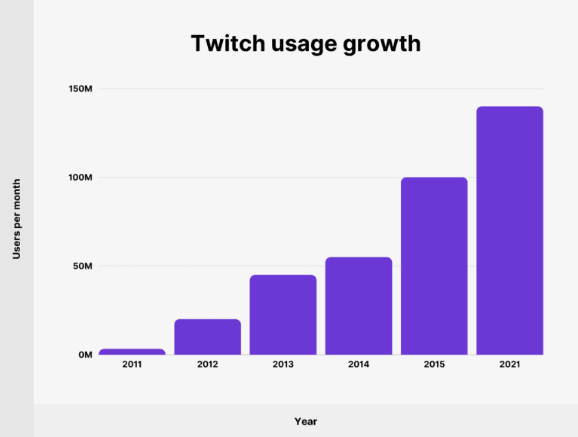
\includegraphics[scale=0.85]{imagens/viabilidadeFinanceira/CrescimentoTwitch.png}
	\fonte{\cite{twitch_growth_statistics}}
\end{figure}

Com 7,4 milhões de \textit{streamers} criando conteúdo a cada mês e um total de 9,2 milhões de \textit{streamers} ativos, fica claro que a comunidade de criadores desempenha um papel fundamental na expansão do \textit{\gls{Twitch}}. Os espectadores do \textit{\gls{Twitch}} assistem coletivamente a uma incrível quantidade de conteúdo, totalizando 1,14 trilhão de minutos assistidos, equivalentes a 1,86 bilhão de horas mensais.

Em termos de receita anual de publicidade, o \textit{\gls{Twitch}} alcançou a marca de US\$ 231,8 milhões, representando mais que o dobro dos US\$ 102,5 milhões registrados em 2017. Além da publicidade, outra fonte significativa de receita para o \textit{\gls{Twitch}} é o sistema de assinaturas. No entanto, a avaliação precisa dessa receita é desafiadora, uma vez que as assinaturas \textit{premium} do \textit{\gls{Amazon Prime}} incluem automaticamente a assinatura \textit{premium} do \textit{\gls{Twitch}}. Estimativas indicam que a receita anual total do \textit{\gls{Twitch}} gira em torno de US\$ 1,54 bilhão.

No que tange à base de usuários, o \textit{\gls{Discord}} ostenta números notáveis, com uma marca impressionante de 140 milhões de usuários ativos mensais, conforme demonstra a Figura \ref{usuariosMensaisDiscord}. Mais notável ainda é o fato de que essa base dobrou no último ano, o que atesta um crescimento substancial e sustentado ao longo do tempo. 

\begin{figure}[H]
    \center
	\caption{\label{fig_sge20}Usuários ativos mensais do Discord}
    \label{usuariosMensaisDiscord}
    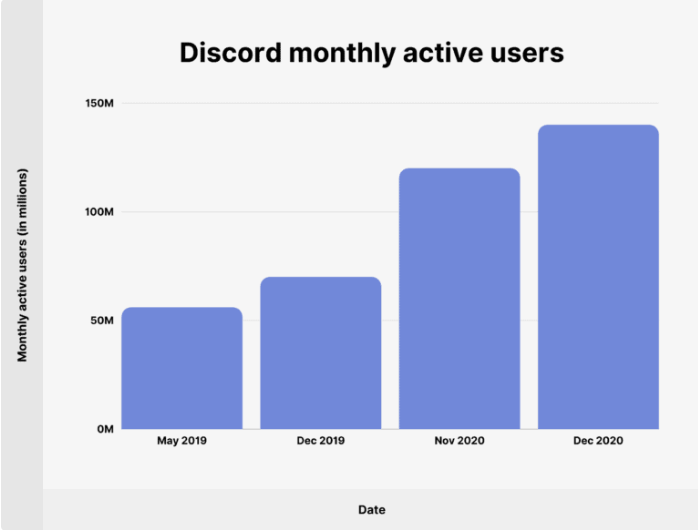
\includegraphics[scale=0.7]{imagens/viabilidadeFinanceira/DiscordActiveUsers.png}
	\fonte{\cite{discord_active_users}}
\end{figure}

No âmbito dos investimentos, o \textit{\gls{Discord}} angariou uma expressiva quantia de financiamento, totalizando US\$ 483,8 milhões. Além disso, o \textit{\gls{Discord}} demonstra sua capacidade de monetização ao gerar uma receita anual considerável, totalizando US\$ 130 milhões. Com uma valoração atual de US\$ 7 bilhões e uma rede de cerca de 13,5 milhões de servidores ativos por semana, o \textit{\gls{Discord}} emerge como um protagonista fundamental no cenário das interações online, consolidando-se como uma das principais plataformas de comunicação no mundo.

\subsection{Análise e Projeção}

Para estimar o crescimento de usuários do projeto, foi adotada como abordagem de análise uma curva normal de crescimento. Estabelecemos como meta de projeção um incremento de 1\% no número de usuários ativos em relação às duas plataformas mencionadas, ao término dos primeiros 12 meses.

A projeção de um aumento de 1\% ao longo do período de 12 meses resultaria em um total de 30.000 usuários ativos na plataforma. Ressalta-se a relevância deste crescimento gradual, o qual segue uma trajetória ascendente que se alinha com as tendências observadas na \textit{\gls{Twitch}} e no \textit{\gls{Discord}}. Cabe destacar que, embora o projeto esteja em estágio inicial e não disponha da mesma base de usuários das plataformas mencionadas, a tendência de crescimento sustentado é promissora.

Com base nas informações disponíveis sobre a \textit{\gls{Twitch}} e o \textit{\gls{Discord}}, é plenamente justificável projetar um aumento gradual para o presente projeto. As referidas plataformas representam notáveis exemplos de sucesso no âmbito do entretenimento online e da comunicação, o que reflete a crescente demanda por tais serviços. Nesse contexto, a estimativa de crescimento de usuários apresentada neste estudo está fundamentada em bases sólidas e aponta para um considerável potencial.

% Despesas
\section{Despesas}

As despesas inerentes ao presente projeto encontram-se intrincadamente associadas a três fontes de destaque, nomeadamente: infraestrutura, recursos humanos e angariação de clientes.

\subsection{Infraestrutura}

Os ônus relativos à infraestrutura do projeto serão integralmente derivados dos serviços providos pela plataforma \textit{\gls{Azure}}, visto que as demais instâncias participantes se pautam pela isenção de custos. A delimitação do preço desses serviços foi efetuada por intermédio da aplicação da Calculadora de Custos \textit{\gls{AzurePricingCalculator}}. Nesse processo de cálculo, foram criteriosamente incorporados os serviços de \textit{\gls{AppService}} e \textit{\gls{AzureSQLDatabase}}, a fim de mensurar com precisão os dispêndios vinculados a tais soluções. A tabela \ref{estimativaAzure} elucida a projeção orçamentária referente à Azure.

\begin{table}[H]
    \setcounter{table}{0}
    \center
	\caption{Custos Azure Services}
    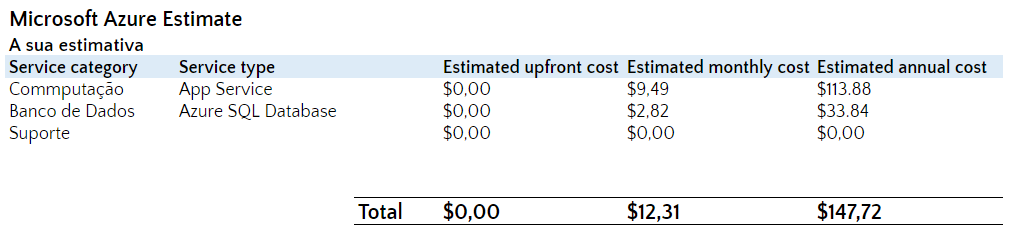
\includegraphics[scale=0.55]{imagens/viabilidadeFinanceira/estimativaAzure.png}
    \label{estimativaAzure}
	\fonte{Azure Pricing Calculator}
\end{table}

De acordo com a estimativa de usuários realizada, foi possível estimar também os custos de infraestrutura gerados, fornecendo uma visualização dessa fonte de despesas, como pode ser visto na tabela \ref{estimativaAzure}.

\subsection{Recursos Humanos}

No contexto de um projeto no âmbito da tecnologia, a apropriação dos recursos financeiros destinados aos elementos humanos compreende uma amplitude abrangente de fatores mutuamente interligados. Estes englobam componentes como a remuneração dos colaboradores, as obrigações fiscais e previdenciárias, as vantagens e benefícios oferecidos, as iniciativas de aperfeiçoamento e o contínuo desenvolvimento profissional. A competente gestão desses recursos assume um papel preponderante, exercendo uma influência crucial no sucesso do empreendimento e na maximização dos aportes investidos.

No que tange às remunerações, os desembolsos podem variar significativamente devido às posições ocupadas e ao nível de especialização dos membros da equipe. Os encargos trabalhistas, abarcando as contribuições sociais e outras obrigações jurídicas, também compõem a soma total dedicada.

A concessão de benefícios, como planos de saúde, auxílios-alimentação e transporte, se converte em um elemento adicional, conferindo um acréscimo financeiro ao montante designado. A capacitação da equipe, mediante a implementação de programas de formação e atualização, insere-se no âmbito do investimento, salvaguardando a manutenção da excelência laboral em um cenário tecnológico em constante mutação.

De acordo com as orientações preconizadas por plataformas especializadas em oportunidades de trabalho, análises de mercado e organizações dedicadas ao recrutamento, os valores correspondentes às despesas podem ser delineados com base em uma média geral:

\begin{itemize}
    \item \textbf{Salário de Estágio}: R\$ 1.500,00;
    \item \textbf{Encargos Trabalhistas (aproximadamente 70\% do salário)}: R\$ 1.050,00;
    \item \textbf{Benefícios (plano de saúde, vale-transporte, vale-alimentação)}: R\$ 300,00.
\end{itemize}

Considerando que a configuração da equipe é constituída por um grupo de seis desenvolvedores em nível de estágio, os montantes financeiros mensais que imperam no cenário comercial foram incorporados à análise, conforme o Quadro \ref{despesasRecursosHumanos}:

\begin{itemize}
    \item Custo base: R\$ 2.800,00
    \item Dias-base: 22 | Dia-hora: 8
    \item Custo-hora: R\$ 15,90
\end{itemize}

\begin{quadro}[H]
\centering
\caption{Despesas dos Recursos Humanos}
\label{despesasRecursosHumanos}
\begin{longtable}{|p{5cm}|p{3cm}|p{3cm}|}
\hline
Despesa & 6 meses & 12 meses
\\\hline
Salário & R\$ 54.000,00 & R\$ 108.000,00\
\\\hline
Encargos Trabalhistas & R\$ 37.800,00 & R\$ 75.600,00\
\\\hline
Benefícios & R\$ 10.800,00 & R\$ 21.600,00\
\\\hline
\end{longtable}
\fonte{Os Autores.}
\end{quadro}

A contabilização das horas referentes ao projeto incorporou a análise de três distintas classificações de requisitos funcionais a serem incorporados: níveis fácil, médio e difícil, organizados em conformidade com a proficiência dos membros da equipe.

Para os requisitos funcionais fáceis, foi tomado como base um tempo de 48 horas de desenvolvimento. Já para os médios foi considerado o tempo de 80 horas de desenvolvimento e, para os difíceis, 160 horas. Tais despesas desempenham um papel preponderante especialmente ao longo da fase de desenvolvimento do projeto. A representação gráfica \ref{maoDeObra} evidencia a apresentação destes cálculos.

\begin{table}[H]
    \center
    \setcounter{table}{1}
	\caption{Mão de Obra Mensal}
    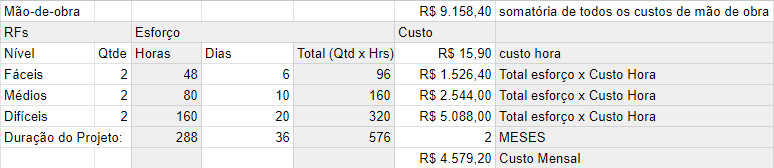
\includegraphics[scale=0.75]{imagens/viabilidadeFinanceira/MaoDeObra.png}
    \label{maoDeObra}
	\fonte{Os autores}
    \setcounter{table}{2}
\end{table}

A tabela \ref{maoDeObra} demonstra a quantidade de horas totais a serem utilizadas no projeto, bem como os custos totais com mão de obra e os custos mensais a serem assumidos. De acordo com o cálculo de horas realizado na tabela, é possível observar que a duração será de 2 meses.

\subsection{Captação de Clientes}

Com vistas a consolidar a estratégia de aquisição de clientes para a plataforma, almeja-se direcionar recursos para atividades de marketing. Isso se concretizará mediante a veiculação de anúncios em plataformas conexas ao público-alvo do projeto, a exemplo do \textit{\gls{Youtube}}, \textit{\gls{Twitch}} e \textit{\gls{Tiktok}}. A ênfase recairá na promoção desses anúncios em conteúdos especialmente voltados ao universo dos jogos eletrônicos, visando estabelecer uma afinidade precisa e maximizar a eficácia das iniciativas na atração de novos usuários para a \textit{GameLocker}.

Ademais, uma possibilidade viável consiste na divulgação nestas plataformas mediante um enfoque mais personalizado, alcançado por meio do estabelecimento de colaborações diretas com os criadores de conteúdo. A concretização destas parcerias seria intermediada por acordos de patrocínio, nos quais eles divulgariam o sistema perante sua audiência.

Dentro do contexto de cada uma das mencionadas plataformas, que permitem valores personalizados de investimento em marketing, estima-se, em um primeiro momento, um aporte de investimento mensal equivalente a R\$ 267,00, culminando, assim, em um montante total de R\$ 800,00 mensais destinado à angariação de novos usuários. Estes valores têm o objetivo de manter a captação de usuários ativa sem que o projeto se torne inviável financeiramente.

% Receitas
\section{Receitas}

Visando assegurar a viabilidade financeira do projeto, foram definidas estratégias de remuneração através de anúncios de banners personalizados. Além disso, foi estabelecido um plano Premium que oferece recursos e benefícios adicionais em comparação com o plano gratuito.

\subsection{Anúncios de banners personalizados}

A implementação de anúncios por meio de banners personalizados surgiu em resposta a dificuldades enfrentadas durante a implementação do \textit{\gls{GoogleAdSense}}. Esta estratégia será empregada até que os problemas relacionados ao baixo tráfego sejam resolvidos. Apesar das adversidades encontradas, os anúncios personalizados oferecem a vantagem de adaptar sua aparência e estilo para se integrar de forma harmoniosa com o tema visual da aplicação. Além disso, proporcionam a capacidade de personalizar os tipos de anúncios exibidos, assegurando assim que o conteúdo publicitário seja relevante para o público-alvo.

\subsection{Plano Premium}

O plano Premium consiste em uma assinatura oferecida aos usuários, proporcionando benefícios exclusivos, tais como bloqueio de anúncios e criações de Arenas de Jogos. Conforme descrito abaixo:

\begin{itemize}
    \item \textbf{Bloqueio de anúncios}: Experiência livre de anúncios, podendo navegar no site sem interrupções de propagandas indesejadas;
     \item \textbf{Criações de Arenas de Jogos}: Inclusão de uma arena de jogos online, com o intuito de proporcionar aos usuários a oportunidade de competir entre si em jogos \textit{\gls{Multiplayer}}, além de criar torneios e interagir com outros jogadores;
\end{itemize}

As assinaturas podem ser efetuadas de forma mensal, permitindo que os usuários cancelem ou alterem sua assinatura a qualquer momento, sem compromisso a longo prazo. Ou anual, adequada para aqueles que desejam se comprometer com o serviço ou produto a longo prazo e estão dispostos a fazer um pagamento adiantado. Opções de planos premium disponíveis descritos abaixo:

\begin{itemize}
    \item \textbf{Assinatura mensal}: R\$ 15,00;
    \item \textbf{Assinatura anual}: R\$ 160,00
\end{itemize}

É perceptível que a opção pela subscrição anual proporciona aos usuários um desconto de aproximadamente 11\% quando comparada à alternativa mensal. Esta estratégia visa não somente otimizar o custo para o cliente, mas também objetiva consolidar uma relação de fidelização ao estender o compromisso de uso ao longo do ano, contribuindo, assim, para a captação de recursos sustentáveis.

O valor mensal estipulado em R\$ 15,00 é estabelecido com o propósito de subsidiar as despesas inerentes à plataforma, ao passo que visa também a assegurar proventos futuros. Destarte, esse montante é calculado de maneira a não onerar excessivamente o usuário final, ao mesmo tempo em que se almeja construir um cenário de lucratividade sustentável para a empreitada.

Com a finalidade de estabelecer esse valor mensal, tomou-se como base a análise realizada no tópico \ref{subsec::publico-alvo_semelhante}, já que as aplicações analisadas oferecem recursos similares dentro dessas subscrições, a exemplo de personalização de perfis, bloqueio de anúncios e acesso a funcionalidades exclusivas, além de possuírem um público-alvo parecido com o da GameLocker, como já foi sugerido.

\subsubsection{Análise das Assinaturas}

Após minuciosa análise dos valores adotados por ambas as plataformas e das vantagens inerentes a cada uma, somada a uma avaliação justa dos ganhos projetados e dos custos operacionais do sistema, é possível deduzir que a tarifa mensal de R\$ 15,00 representa um montante equitativo a ser requisitado dos consumidores. Este valor permanece em consonância com as tarifas observadas em sistemas similares, ao mesmo tempo que se esforça por manter um nível de acessibilidade abrangente, abarcando assim uma considerável parcela de potenciais usuários.

% Graficos
\subsection{Gráficos dos Cenários}

Os gráficos a seguir apresentam uma visão abrangente das projeções financeiras para um período de 12 meses, considerando os cenários pessimista, realista e otimista.

Na Figura \ref{cenarioRealista}, podemos observar que, em um cenário realista, a possibilidade de alcançar o ponto de equilíbrio ocorre em 10 meses, resultando em um lucro de R\$ 20.000 ao final do período de 12 meses.

Entretanto, a Figura \ref{cenarioPessimista} destaca o cenário pessimista do projeto, no qual não se vislumbra a capacidade de atingir o ponto de equilíbrio dentro do prazo de 12 meses, ocorrendo apenas próximo ao décimo terceiro mês de projeto, com um lucro de R\$1.217,00

Por último, a Figura \ref{cenarioOtimista} ilustra o cenário otimista do projeto, onde os lucros apresentam um crescimento mais rápido e o ponto de equilíbrio é alcançado mais cedo, precisamente em 9 meses e meio. Ao término dos 12 meses, é esperado um lucro de aproximadamente R\$ 25.000,00.

\begin{figure}[H]
    \center
	\caption{\label{fig_sge20}Gráfico do Cenário Realista}
    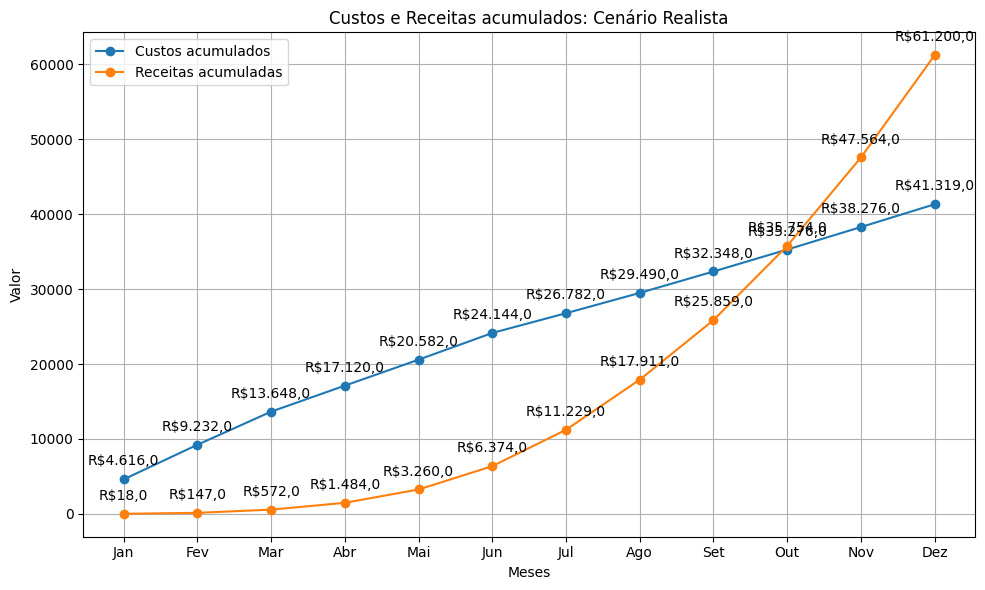
\includegraphics[scale=0.60]{imagens/viabilidadeFinanceira/Projeção-Receita_Custos-Realista.png}
    \label{cenarioRealista}
	\fonte{Os autores}
\end{figure}

\begin{figure}[H]
        \center
	\caption{\label{fig_sge20}Gráfico do Cenário Pessimista}
    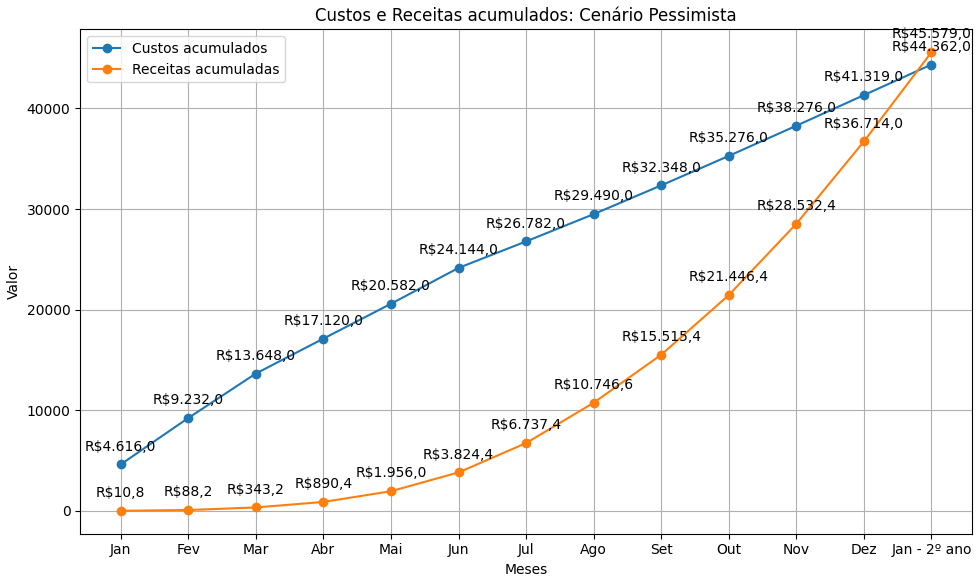
\includegraphics[scale=0.60]{imagens/viabilidadeFinanceira/Projeção-Receita_Custos-Pessimista.png}
    \label{cenarioPessimista}
	\fonte{Os autores}
\end{figure}

\begin{figure}[H]
        \center
	\caption{\label{fig_sge20}Gráfico do Cenário Otimista}
    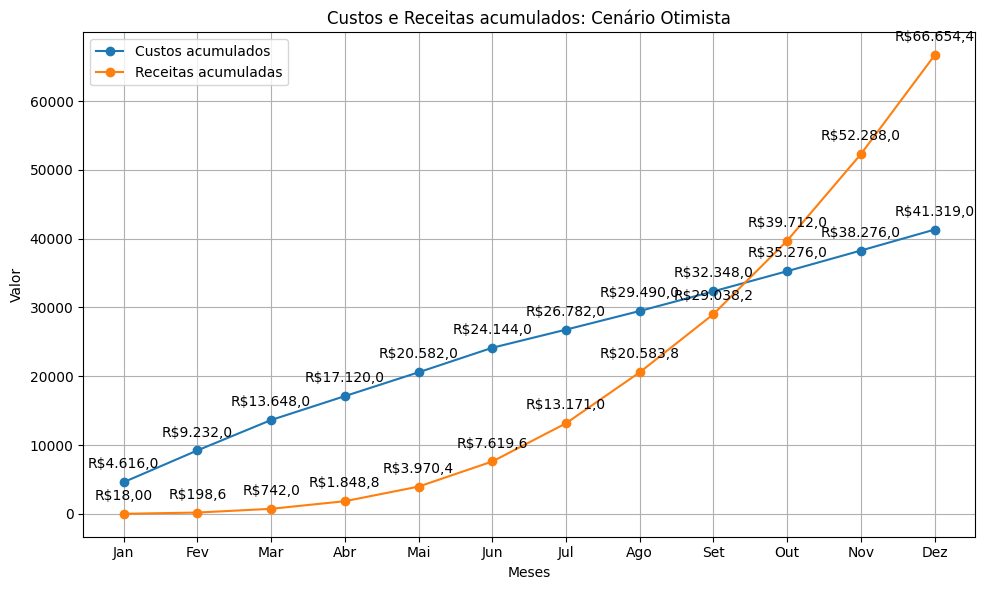
\includegraphics[scale=0.60]{imagens/viabilidadeFinanceira/Projeção-Receita_Custos-Otimista.png}
    \label{cenarioOtimista}
	\fonte{Os autores}
\end{figure}

% Descartes / Escolhas
\chapter{Descartes/Escolhas}

Este capítulo busca descrever as mudanças relacionadas às regras de negócio e funcionalidades do projeto, divididas em descartes e escolhas. Além disso, são citadas algumas implementações futuras, que podem ser incluídas no projeto mesmo após sua conclusão.

\section{Descartes}

Uma funcionalidade que foi deliberadamente descartada reside na capacidade de conectar deliberadamente as contas e os perfis dos usuários com suas conquistas e progressos em outras plataformas, exemplificadas pela \textit{\gls{Steam}} e \textit{\gls{Microsoft}}. A incorporação dessa funcionalidade implicaria em um grau considerável de complexidade, agravado pelo desafio de obter acesso à \ac{api} da \textit{\gls{Steam}}, uma circunstância que poderia acarretar complicações suplementares no decorrer do processo de desenvolvimento do projeto. Portanto, essa funcionalidade foi excluída da abordagem, a fim de garantir um escopo mais gerenciável e alinhado com os objetivos principais estabelecidos.

A implementação do anúncio \textit{\gls{GoogleAdSense}} tornou-se inviável devido a problemas existentes, notadamente a insuficiência de tráfego no site. A ausência de tráfego relevante é um problema complexo, envolvendo questões como otimização de mecanismos de busca (SEO), qualidade do conteúdo e estratégias de marketing digital. Nesse cenário, tornou-se claro que a implementação do \textit{AdSense} não era viável no momento presente. O baixo tráfego do site comprometeria a eficácia dos anúncios, levando a baixas taxas de visualizações e, por conseguinte, a receitas insignificantes.

Outra funcionalidade adicional que foi descartada relaciona-se com a disponibilização de notícias relevantes no contexto dos jogos eletrônicos. Isso abrangeria aspectos como a repercussão de novos lançamentos e eventos relacionados ao universo dos jogos.

\section{Escolhas}

A escolha de se implementar um sistema \textit{Web} está diretamente relacionada ao fato de que a grande maioria dos jogos está disponível para PC, além da forte presença da \textit{\gls{Steam}}, que comumente é acessada em computadores. Por isso, espera-se que a maioria dos usuários da plataforma GameLocker a acessem em navegadores \textit{Web}.%INCLUIR FONTE

Outra decisão a se apontar foi a de não armazenar o histórico de mensagens da arena de jogos, que se dá por dois fatores principais: recursos computacionais e complexidade de desenvolvimento. O primeiro se justifica pelo fato de que manter armazenar um número muito elevado de mensagens da arena poderia ser muito custoso computacionalmente. O segundo tem relação com o cronograma do projeto, já que desenvolver uma maneira de armazenar essas mensagens poderia atrasar os prazos definidos.

\section{Implementações Futuras}

Como implementação futura, é possível citar a publicação de jogos diretamente na plataforma, permitindo que pequenos desenvolvedores de jogos conseguissem um espaço para divulgá-los livremente. Esta funcionalidade foi sugerida pelo professor orientador do primeiro semestre da disciplina, Carlos Henrique Veríssimo, como uma maneira de propagar os jogos desenvolvidos por alunos de cursos técnicos.

Apesar do \textit{\gls{GoogleAdSense}} ter sido descartado, a equipe tem o planejamento de implementar essa estratégia de anúncio assim que o tráfego da aplicação melhorar. A implementação do \textit{\gls{GoogleAdSense}}, foram considerados fatores cruciais, como o perfil do público-alvo da aplicação, de modo a aproveitar as oportunidades de monetização e direcionar anúncios relevantes aos visitantes da plataforma, proporcionando uma experiência agradável e maximizando o potencial de geração de receita. Foi estabelecido adotar o modelo de remuneração \ac{cpm} como forma de monetização pelo número de vezes que os anúncios seriam exibidos na plataforma, a cada mil impressões.

Outra implementação futura seria a disponibilização de uma versão \textit{mobile} da aplicação, para assim atingir uma maior gama de usuários e otimizando a usabilidade do sistema.

% Testes
\chapter{Testes}
Este capítulo tem como objetivo apresentar os testes realizados durante o desenvolvimento do projeto, que auxiliaram a fazer um controle de qualidade da aplicação com maior precisão.

% Testes Unitários
\section{Testes Unitários}
Esta seção tem como objetivo demonstrar os testes unitários realizados tanto no \textit{\gls{Back-end}} quanto no \textit{\gls{Front-end}}, que auxiliaram a validar o funcionamento desejado das funções desenvolvidas.

\subsection{Back-end}
No desenvolvimento dos testes unitários do \textit{\gls{Back-end}}, foi utilizado o pacote \textit{XUnit}, que é uma ferramenta \textit{open-source} de testes para \gls{.NET}.

A ferramenta empregada para verificar a cobertura dos testes realizados foi a \textit{Fine Code Coverage}. Na figura \ref{coverageGeralBack}, é possível observar a cobertura total dos testes na aplicação. Já a figura \ref{coverageBack} demonstra a cobertura dos testes dividida entre as camadas da aplicação.

\begin{figure}[H]
    \caption{Cobertura Geral dos testes}
	\centering
	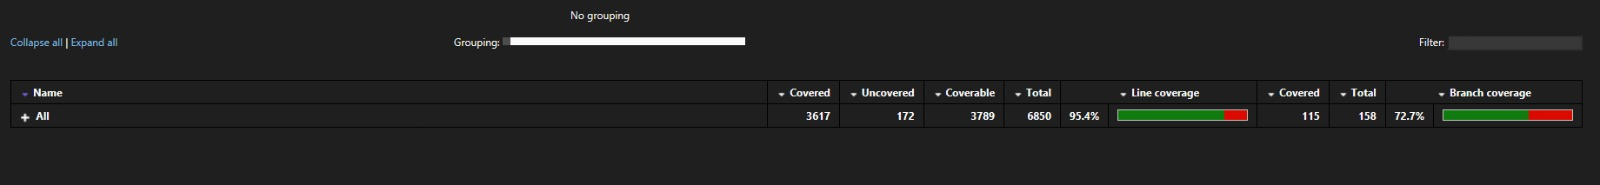
\includegraphics[width=1\textwidth]{imagens/testes/TestesUnitariosBackend/coverageGeral.jpeg}
    \label{coverageGeralBack}
	\fonte{Os autores}
\end{figure}

\begin{figure}[H]
    \caption{Cobertura dos testes por camada}
	\centering
	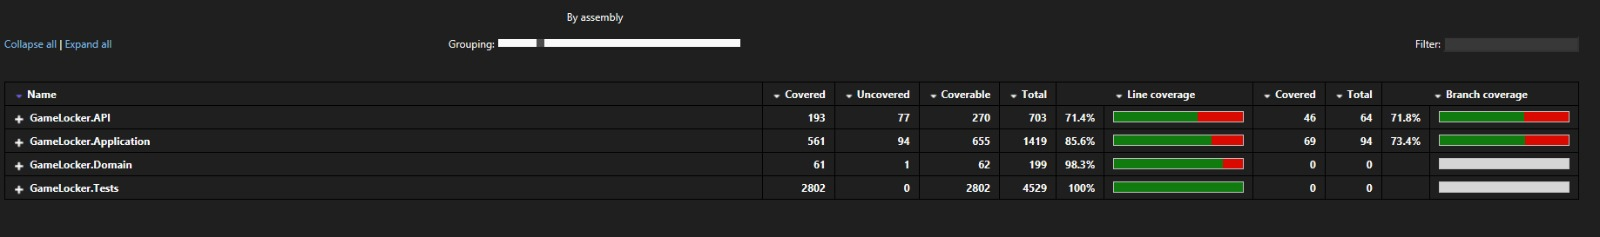
\includegraphics[width=1\textwidth]{imagens/testes/TestesUnitariosBackend/coverage.jpeg}
	\label{coverageBack}
    \fonte{Os autores}
\end{figure}
\pagebreak

A figura \ref{resultadoTestesBack} apresenta o resultado da execução dos testes, demonstrando sucesso em todos eles.

\begin{figure}[H]
    \caption{Resultado dos testes}
	\centering
	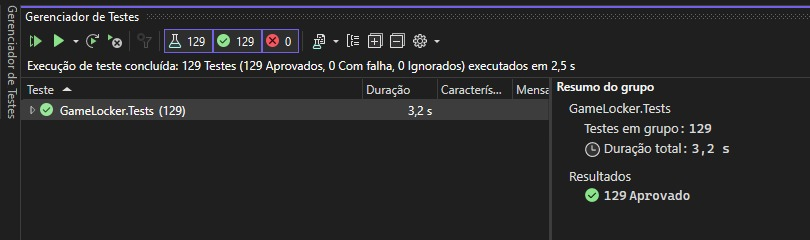
\includegraphics[width=1\textwidth]{imagens/testes/TestesUnitariosBackend/resultado.jpeg}
    \label{resultadoTestesBack}
	\fonte{Os autores}
\end{figure}

\subsection{Front-end}
Para auxiliar no desenvolvimento dos testes unitários do \textit{\gls{Front-end}}, foram utilizadas as bibliotecas \textit{Jest} e \textit{React Testing Library}.

A figura \ref{coverageFront} demonstra a cobertura de testes por página da aplicação. Já a figura \ref{coverageGeralFront} apresenta a cobertura geral, em todos os arquivos.

\begin{figure}[H]
    \caption{Cobertura dos testes por página}
	\centering
	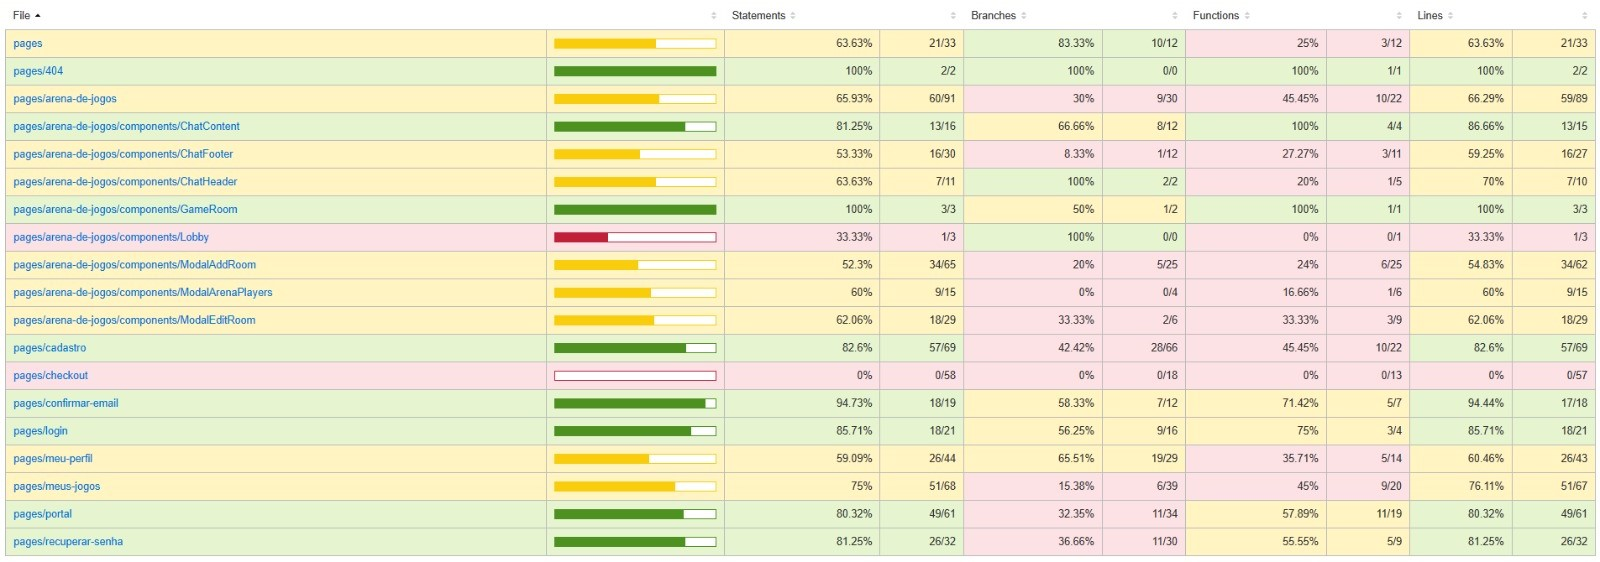
\includegraphics[width=1\textwidth]{imagens/testes/TestesUnitariosFrontend/coverageFront.jpeg}
	\label{coverageFront}
    \fonte{Os autores}
\end{figure}

\begin{figure}[H]
    \caption{Cobertura Geral dos testes}
	\centering
	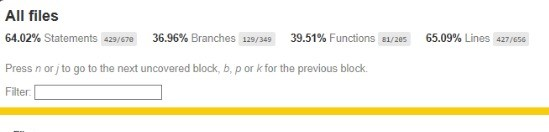
\includegraphics[width=1\textwidth]{imagens/testes/TestesUnitariosFrontend/coverageGeralFront.jpeg}
	\label{coverageGeralFront}
    \fonte{Os autores}
\end{figure}

Na figura \ref{resultadosTestesFront} é possível observar o resultado da execução dos testes, demonstrando êxito em sua totalidade.

\begin{figure}[H]
    \caption{Resultados dos testes}
	\centering
	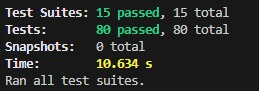
\includegraphics[width=1\textwidth]{imagens/testes/TestesUnitariosFrontend/resultadosTestesFront.jpeg}
	\label{resultadosTestesFront}
    \fonte{Os autores}
\end{figure}

% Planos de Teste
\section{Plano de Testes}

O propósito da presente seção reside na apresentação pormenorizada dos fluxos a serem adotados no âmbito dos planos de testes do sistema, tendo como desiderato a verificação da operacionalidade dos casos de uso preeminentes.

\subsubsection{Teste de Funcionalidade de Registro e Login}
\begin{enumerate}

\item{\textbf{Nome do projeto:}}
Verificando a funcionalidade de registro e login da aplicação \textit{Gamelocker};

\item{\textbf{Resumo:}}
A aplicação \textit{GameLocker} apresenta um amplo conjunto de funcionalidades. No entanto, como é comum em qualquer aplicação, é fundamental que as funções essenciais de registro e login ocorram de maneira adequada. A correta execução dessas etapas é crucial, pois permite que os usuários acessem suas contas registradas, abrindo caminho para a utilização efetiva de todas as demais funcionalidades disponíveis;

\item{\textbf{Pessoas envolvidas:}}
Os integrantes do grupo de desenvolvedores se juntaram em duplas;

\item{\textbf{Funcionalidades a serem testadas:}}
As páginas de registro e login foram selecionadas como foco dos testes das funcionalidades, visando não apenas verificar a correta execução das funções propostas, mas também avaliar a usabilidade dessas páginas;

\item{\textbf{Local dos testes:}}
Os testes serão realizados nas residências dos integrantes, em horários acordados por eles. Não tendo necessidade de se utilizar um ambiente em conjunto para tal;

\item{\textbf{Recursos necessários:}}
Os recursos necessários serão fornecidos pelos próprios testadores, que serão responsáveis por criar registros e realizar o login no site. Para facilitar o armazenamento e o acesso aos resultados de cada teste para cada membro do grupo, os testadores deverão utilizar uma ferramenta que permita o armazenamento centralizado e o acesso fácil aos dados obtidos durante o processo de testes;

\item{\textbf{Critérios usados para teste:}}
\\
\textbf{Que teste será feito:} 
\begin{itemize}
\item O teste realizado compreende uma sequência de etapas. Primeiramente, é necessário acessar a página de cadastro e preencher corretamente todas as informações requeridas, observando as diretrizes e regras estabelecidas, incluindo requisitos como tamanho mínimo de senha e escolha adequada de nome de usuário, entre outros critérios definidos. Após o preenchimento bem-sucedido do formulário de cadastro, confirmar o endereço de e-mail associado à conta. Em seguida, acessar a página de login, inserir os dados previamente cadastrados e confirmar a funcionalidade do sistema. 
\end{itemize}

\textbf{Como aplicar o teste:} 
\\
\\\textbf{Fluxo de Cadastro:}
\begin{enumerate}
\item Inserir o campo de nome;
\item Inserir o campo de sobrenome;
\item Inserir o campo de data de nascimento;
\item Inserir o campo de telefone;
\item Inserir o campo de nome de usuário;
\item Caso haja algum campo incorreto durante o processo de registro ou login, exibir mensagens de erro específicas no modal correspondente;
\item Com todos os campos preenchidos corretamente, o botão de continuar o cadastro estará habilitado;
\item Clicar no botão continuar;
\item Inserir o campo de e-mail;
\item Inserir a campo de senha;
\item Preencher o campo de confirmar senha;
\item Clicar no botão de cadastrar;
\item Caso haja algum campo incorreto durante o processo de registro ou login, exibir mensagens de erro específicas no modal correspondente;
\item Se todas as informações estiverem corretamente preenchidas pelo usuário, será solicitada a confirmação do endereço de e-mail.
\item Após a confirmação, um modal será exibido, informando que o cadastro foi realizado com sucesso.
\item Em seguida, o sistema redirecionará o usuário para a tela de login, onde ele poderá realizar o acesso à sua conta.
\end{enumerate}

\textbf{Fluxo de Login:}
\begin{enumerate}
\item Inserir o campo de e-mail;
\item Inserir o campo de senha;
\item Clicar no botão de ``Entrar'', caso algum dos campos preenchidos esteja em desacordo com as informações fornecidas durante o cadastro, o usuário deverá ser prontamente notificado;
\item Caso os campos estejam corretamente preenchidos, o usuário será redirecionado para a tela de portal.
\end{enumerate}

\item{\textbf{Riscos:}}
\begin{itemize}
\item No caso de algum dos testadores não conseguir realizar suas atividades, é imprescindível que os demais sejam informados para que seja feita uma organização adequada e garantir que todas as etapas de teste sejam concluídas;
\item Devido a problemas de hospedagem, ocorrer uma falta de conexão com o \textit{\gls{Back-end}}, exigindo a realização de testes em ambiente local.
\end{itemize}

\item{\textbf{Como os resultados do teste serão divulgados:}}
Ao final desta seção de planejamento dos testes, encontra-se um quadro que indica o resultado de cada um dos testes realizados, classificando-os como sucesso ou falha. Caso ocorra uma falha, será apresentada a motivação subjacente a ela.
\end{enumerate}

\subsubsection{Teste de Funcionalidade do Sistema de Reviews}
\begin{enumerate}

\item{\textbf{Nome do projeto:}}
Verificando a funcionalidade do sistema de reviews;

\item{\textbf{Resumo:}}
A funcionalidade central do site \textit{GameLocker} baseia-se em avaliações. Portanto, é necessário que essa funcionalidade funcione corretamente, a fim de garantir que o site cumpra o que se propôs a realizar;

\item{\textbf{Pessoas envolvidas:}}
Os integrantes do grupo de desenvolvedores se juntaram em duplas;

\item{\textbf{Funcionalidades a serem testadas:}}
Todas as funções relacionadas às avaliações foram submetidas a testes (Criação, Visualização, Edição e Exclusão) a fim de garantir uma usabilidade correta da proposição do site;

\item{\textbf{Local dos testes:}}
Os testes serão realizados nas residências dos integrantes, em horários acordados por eles. Não tendo necessidade de se utilizar um ambiente em conjunto para tal;

\item{\textbf{Recursos necessários:}}
Os recursos necessários serão fornecidos pelos próprios testadores, que serão responsáveis por criar registros e realizar o login no site. Para facilitar o armazenamento e o acesso aos resultados de cada teste para cada membro do grupo, os testadores deverão utilizar uma ferramenta que permita o armazenamento centralizado e o acesso fácil aos dados obtidos durante o processo de testes;

\item{\textbf{Critérios usados para teste:}}
\\
\textbf{Que teste será feito:} 
\begin{itemize}
\item Criação de uma review para um jogo específico escolhido pelo usuário, adicionando todos os dados necessários;
\item Visualização dessa revisão na tela de perfil de usuário;
\item Edição dessa review, atualizando na tela de perfil;
\item Remoção dessa revisão, a excluindo.
\end{itemize}

\textbf{Como aplicar o teste:} 
\\
\textbf{Fluxo de Criação:}
\begin{enumerate}
\item Escolher o jogo no qual será feita a review;
\item Inserir um comentário sobre esse jogo;
\item Inserir uma nota de 0 a 10;
\item Inserir o status do jogo (Jogando, Dropado, Zerado, Desejado);
\item Finalizar a review;
\item Com tudo ocorrendo da maneira correta, a review terá sido adicionada ao perfil do usuário.
\end{enumerate}

\textbf{Fluxo de Visualização:}
\begin{enumerate}
\item Entrar na tela de meu perfil;
\item Buscar qual review é desejado para visualização;
\item Clicar na review e visualizar os comentários, status e nota dada.
\end{enumerate}

\textbf{Fluxo de Edição:}
\begin{enumerate}
\item Entrar na tela de meu perfil;
\item Buscar qual review é desejado para edição;
\item Clicar na review e visualizá-la por completo;
\item Alterar os campos desejados, tais como mudar a nota de 6 para 10;
\item Salvar as alterações;
\item Fechar o modal de review.
\end{enumerate}

\textbf{Fluxo de Exclusão:}
\begin{enumerate}
\item Entrar na tela de meu perfil;
\item Buscar qual review é desejado para remoção;
\item Clicar na review e visualizá-la por completo;
\item Selecionar a opção de excluir.
\end{enumerate}

\item{\textbf{Riscos:}}
\begin{itemize}
\item No caso de algum dos testadores não conseguir realizar suas atividades, é imprescindível que os demais sejam informados para que seja feita uma organização adequada e garantir que todas as etapas de teste sejam concluídas;
\item Devido a problemas de hospedagem, ocorrer uma falta de conexão com o \textit{\gls{Back-end}}, exigindo a realização de testes em ambiente local.
\end{itemize}

\item{\textbf{Como os resultados dos testes serão divulgados:}}
Ao final desta seção de planejamento dos testes, encontra-se um quadro que indica o resultado de cada um dos testes realizados, classificando-os como sucesso ou falha. Caso ocorra uma falha, será apresentada a motivação subjacente a ela.
\end{enumerate}

\subsubsection{Teste de Funcionalidade de Pagamento de Assinatura}

\begin{enumerate}

\item{\textbf{Nome do projeto:}}
Testando a Funcionalidade de Pagamento de Assinatura da aplicação \textit{Gamelocker};

\item{\textbf{Resumo:}}
O teste tem como objetivo verificar a funcionalidade do sistema de pagamento de assinatura do \textit{GameLocker}, garantindo que os usuários possam se inscrever, fornecer informações de pagamento corretas e segura, e ter acesso aos serviços premium após o pagamento;

\item{\textbf{Pessoas envolvidas:}}
Os integrantes do grupo de desenvolvedores se juntaram em duplas;

\item{\textbf{Funcionalidades a serem testadas:}}
Na página de inscrição do sistema, garantir que o formulário de inscrição esteja completo e funcional, permitindo aos usuários escolher o tipo de assinatura desejada. Em relação ao processo de pagamento, testar o funcionamento da integração com a \gls{api} do \gls{MercadoPago}, enquanto se verifica rigorosamente se os detalhes do cartão são criptografados e protegidos para assegurar a segurança dos dados. Além disso, após o pagamento bem-sucedido, confirmar se os usuários recebem uma confirmação, proporcionando uma garantia adicional da transação, e se eles têm acesso imediato aos recursos premium, demonstrando a eficiência do processo de ativação;

\item{\textbf{Local dos testes:}}
Os testes serão realizados nas residências dos integrantes, em horários acordados por eles. Não tendo necessidade de se utilizar um ambiente em conjunto para tal;

\item{\textbf{Recursos necessários:}}
Um ambiente de testes isolado do ambiente de produção, evitando transações reais. Para simular cenários diversos, utilizar cartões de crédito de teste fornecidos pelo provedor do gateway e explorar emuladores de pagamento. O acesso à documentação técnica completa do gateway, incluindo informações sobre endpoints de API, formatos de dados, códigos de erro e exemplos de solicitações e respostas. Além disso, um ambiente de teste para o sistema, permitindo simular interações de usuários, implementar registros detalhados no sistema, rastreando todas as interações com o gateway de pagamento, para diagnosticar falhas durante os testes;

\item{\textbf{Critérios usados para teste:}}
\\
\textbf{Que teste será feito:} 
\begin{itemize}
\item Inserção dos dados no formulário de assinatura, incluindo uma verificação da integridade dos dados inseridos;
\item Testes rigorosos para as funcionalidades antifraude do gateway. Isso inclui verificações detalhadas do CVV, visando identificar e bloquear transações fraudulentas;
\item Simular diferentes cenários de pagamento para testar a eficácia do sistema. Isso envolve a realização de testes para transações bem-sucedidas, identificação de falhas no pagamento e processos de reembolso.
\item Verificar o acesso imediato aos recursos disponíveis aos usuários \textit{premiums};
\end{itemize}

\item{\textbf{Riscos:}}
\begin{itemize}
\item No caso de algum dos testadores não conseguir realizar suas atividades, é imprescindível que os demais sejam informados para que seja feita uma organização adequada e garantir que todas as etapas de teste sejam concluídas;
\item Problemas de processamento de pagamento que podem atrasar o acesso dos usuários aos serviços premium;
\item Erros de segurança que podem comprometer as informações de pagamento dos usuários.
\end{itemize}

\item{\textbf{Como os resultados do teste serão divulgados:}}
Ao final desta seção de planejamento dos testes, encontra-se um quadro que indica o resultado de cada um dos testes realizados, classificando-os como sucesso ou falha. Caso ocorra uma falha, será apresentada a motivação subjacente a ela.
\end{enumerate}

\subsubsection{Teste de Funcionalidade da Arena de Jogos}
\begin{enumerate}

\item{\textbf{Nome do projeto:}}
Verificando a funcionalidade da Arena de Jogos da aplicação \textit{Gamelocker};

\item{\textbf{Resumo:}}
O teste visa verificar a funcionalidade das Arenas de Jogos no \textit{GameLocker}. Isto inclui garantir que os usuários possam criar salas, configurar regras de jogos e se comunicar por meio de chats. Além disso, será verificado se os administradores têm controle efetivo sobre as salas e se os jogadores podem participar e interagir de forma adequada;

\item{\textbf{Pessoas envolvidas:}}
Os integrantes do grupo de desenvolvedores se juntaram em duplas;

\item{\textbf{Funcionalidades a serem testadas:}}
\begin{itemize}
\item Verificar se os usuários podem criar salas, especificar o tipo de jogo, o número de jogadores e outras configurações relevantes;
\item Garantir que cada sala tenha um chat funcional para permitir a comunicação entre os jogadores durante o jogo;
\item Verificar se os administradores têm controle efetivo sobre a sala, podendo modificar as configurações da sala conforme necessário.
\item Verificar se apenas usuários premium podem criar salas.
\end{itemize}

\item{\textbf{Local dos testes:}}
Os testes serão realizados nas residências dos integrantes, em horários acordados por eles. Não tendo necessidade de se utilizar um ambiente em conjunto para tal;

\item{\textbf{Recursos necessários:}}
Os recursos necessários serão fornecidos pelos próprios testadores, que serão responsáveis por criar registros e realizar o login no site. Para facilitar o armazenamento e o acesso aos resultados de cada teste para cada membro do grupo, os testadores deverão utilizar uma ferramenta que permita o armazenamento centralizado e o acesso fácil aos dados obtidos durante o processo de testes;

\item{\textbf{Critérios usados para teste:}}
\\
\textbf{Que teste será feito:} 
\begin{itemize}
\item Verificar se os usuários premium podem criar salas com sucesso;
\item Testar a implementação do chat, incluindo a capacidade de enviar mensagens e \textit{emojis};
\item Avaliar se os administradores têm controle total sobre as configurações da sala.
\end{itemize}

\item{\textbf{Riscos:}}
\begin{itemize}
\item No caso de algum dos testadores não conseguir realizar suas atividades, é imprescindível que os demais sejam informados para que seja feita uma organização adequada e garantir que todas as etapas de teste sejam concluídas;
\item Devido a problemas de hospedagem, ocorrer uma falta de conexão com o \textit{\gls{Back-end}}, exigindo a realização de testes em ambiente local.
\end{itemize}

\item{\textbf{Como os resultados do teste serão divulgados:}}
Ao final desta seção de planejamento dos testes, encontra-se um quadro que indica o resultado de cada um dos testes realizados, classificando-os como sucesso ou falha. Caso ocorra uma falha, será apresentada a motivação subjacente a ela.
\end{enumerate}

\subsubsection{Quadro de resultados dos testes}
\begin{quadro}[H]
\centering
\caption{Resultados dos Testes}
\label{tab:resultadoteste}
\begin{longtable}{|p{10cm}|p{3cm}|}
\hline
\centering Teste & \centering Resultado
\hline
Funcionalidade de Registro e Login & Sucesso
\\\hline
Funcionalidade do Sistema de Reviews & Sucesso
\\\hline
Funcionalidade de Pagamento de Assinatura & Sucesso
\\\hline
Funcionalidade da Arena de Jogos & Sucesso
\\\hline
\end{longtable}
\fonte{Os Autores.}
\end{quadro}

\section{Testes de Segurança}
Esta seção demonstra os testes de segurança nos quais a aplicação deve ser aprovada, de acordo com as regras da disciplina, buscando garantir uma maior proteção do sistema.

\subsection{Teste de SSL}
Foi utilizada a plataforma SSL Labs \url{https://www.ssllabs.com/ssltest/} para realização deste teste.

Na figura \ref{testeSSL}, é possível observar que a aplicação GameLocker recebeu nota A+ na verificação realizada, demonstrando uma forte segurança na comunicação entre o domínio do site e os navegadores, de forma criptografada.

\begin{figure}[H]
        \center
	\caption{\label{fig_sge20}Resultado do teste de SSL}
    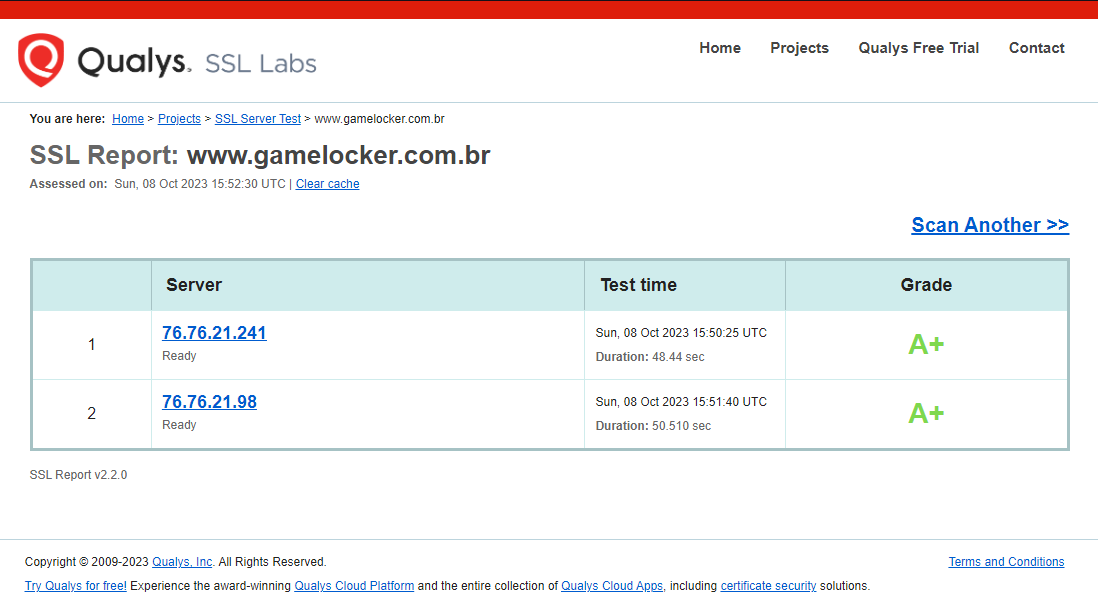
\includegraphics[scale=0.50]{imagens/testes/TESTESSL.png}
    \label{testeSSL}
	\fonte{Os autores}
\end{figure}

\subsection{Teste de Headers}
Este teste tem como objetivo verificar a segurança dos \gls{Headers} nas requisições \ac{https} realizadas pela aplicação. Para isso, foi utilizada a plataforma Security Headers, disponível em: \url{securityheaders.io}

A figura \ref{testeHeaders} apresenta o resultado do teste realizado, indicando um nível satisfatório de segurança nos \gls{Headers} utilizados na aplicação.

\begin{figure}[H]
    \center
	\caption{\label{fig_sge20}Resultado do teste de Headers}
    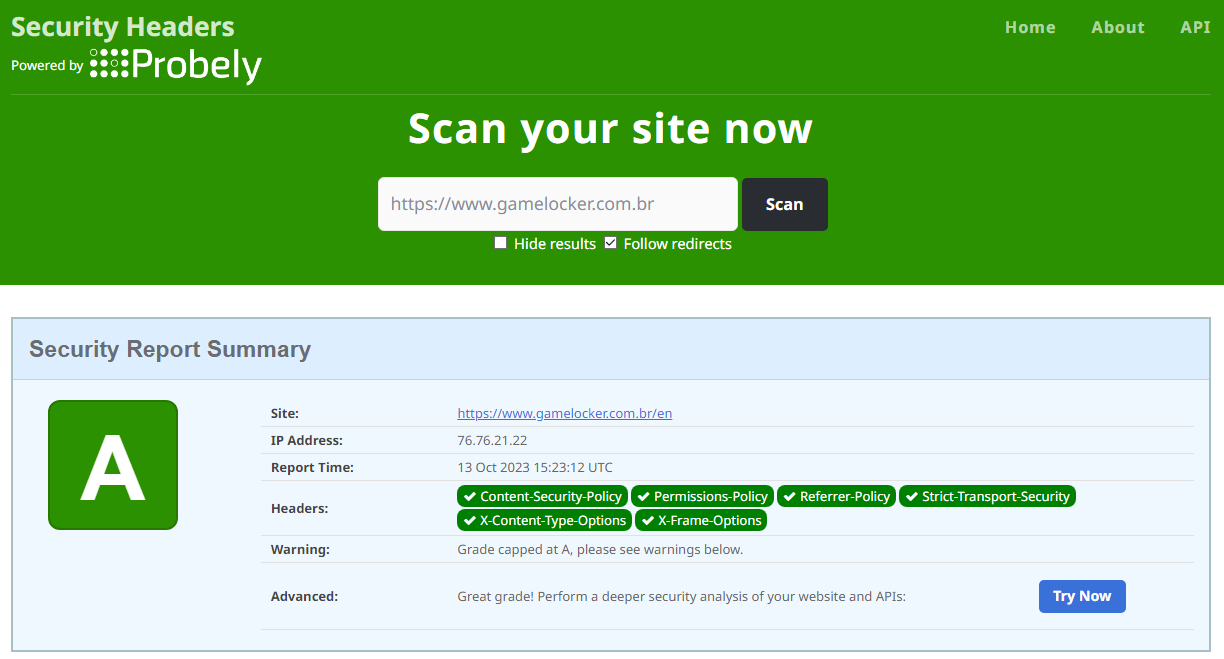
\includegraphics[scale=0.45]{imagens/testes/TESTEHEADERS.png}
    \label{testeHeaders}
	\fonte{Os autores}
\end{figure}

% Links
\chapter{Links do projeto}\label{LinksProjeto}

\begin{figure}[H]
	\centering
	
\includegraphics[width=0.25\textwidth]{imagens/links/aplicacaoQRCode.png}
	\caption{Link da Aplicação}
    \url{https://www.gamelocker.com.br/}
\end{figure}

\begin{figure}[H]
	\centering
	
\includegraphics[width=0.25\textwidth]{imagens/links/blogQRCode.png}
	\caption{Link do Blog}
    \url{https://equipegamelocker.blogspot.com/}
\end{figure}

\begin{figure}[H]
	\centering
	
\includegraphics[width=0.25\textwidth]{imagens/links/svnQRCode.png}
	\caption{Link do SVN}
    \url{https://svn.spo.ifsp.edu.br/svn/a6pgp/S202301-PI-MAT/GameLocker/}
\end{figure}

\begin{figure}[H]
	\centering
	
\includegraphics[width=0.25\textwidth]{imagens/links/youtubeQRCode.png}
	\caption{Link do Youtube}
    \url{https://www.youtube.com/channel/UCdW7IEDJjkzY7mxmha7Qcuw}
\end{figure}

\begin{figure}[H]
	\centering
	
\includegraphics[width=0.25\textwidth]{imagens/links/githubFrontQRCode.png}
	\caption{Link do GitHub - Front-end}
    \url{https://github.com/LuKezLima/game-locker}
\end{figure}

\begin{figure}[H]
	\centering
	
\includegraphics[width=0.25\textwidth]{imagens/links/githubBackQRCode.png}
	\caption{Link do GitHub - Back-end}
    \url{https://github.com/PedroBoscachi/Backend-game-locker}
\end{figure}

\begin{figure}[H]
	\centering
	
\includegraphics[width=0.25\textwidth]{imagens/links/SwaggerQRCode.png}
	\caption{Link do Swagger com os Endpoints}
    \url{https://gamelockerapi.azurewebsites.net/swagger/index.html}
\end{figure}

% \begin{itemize}
% 	\item \textit{Link} do \textit{overleaf}
% \end{itemize}
% \begin{figure}[!h]
% 	
\includegraphics[width=0.15\textwidth]{imagens/links/overleafQRCode.png}\\
% 	\url{https://www.overleaf.com/read/ctrwsthtrwtt}.
% \end{figure}

\pagebreak

% Referências bibliográficas
\bibliography{referencias}

% ----------------------------------------------------------
% Glossário
% ----------------------------------------------------------
%
%
\ifdef{\printnoidxglossary}{
    \addcontentsline{toc}{chapter}{GLOSSÁRIO}
    \printnoidxglossary[style=glossario]
    %\printglossaries
}{}

% ----------------------------------------------------------
% Apêndices
% Documentos gerados pelo próprio autor
% ----------------------------------------------------------

% ---
% Inicia os apêndices
% ---
\begin{apendicesenv}

% Imprime uma página indicando o início dos apêndices
\partapendices
\chapter{Protótipo}
\label{apendice-prototipo}

Este apêndice apresenta um registro dos protótipos de alta fidelidade desenhados para o projeto.

Na Figura \ref{prototipoLandingPage} é apresentado o protótipo da 1º parte da tela de Landing Page.

\begin{figure}[H]
	\centering
	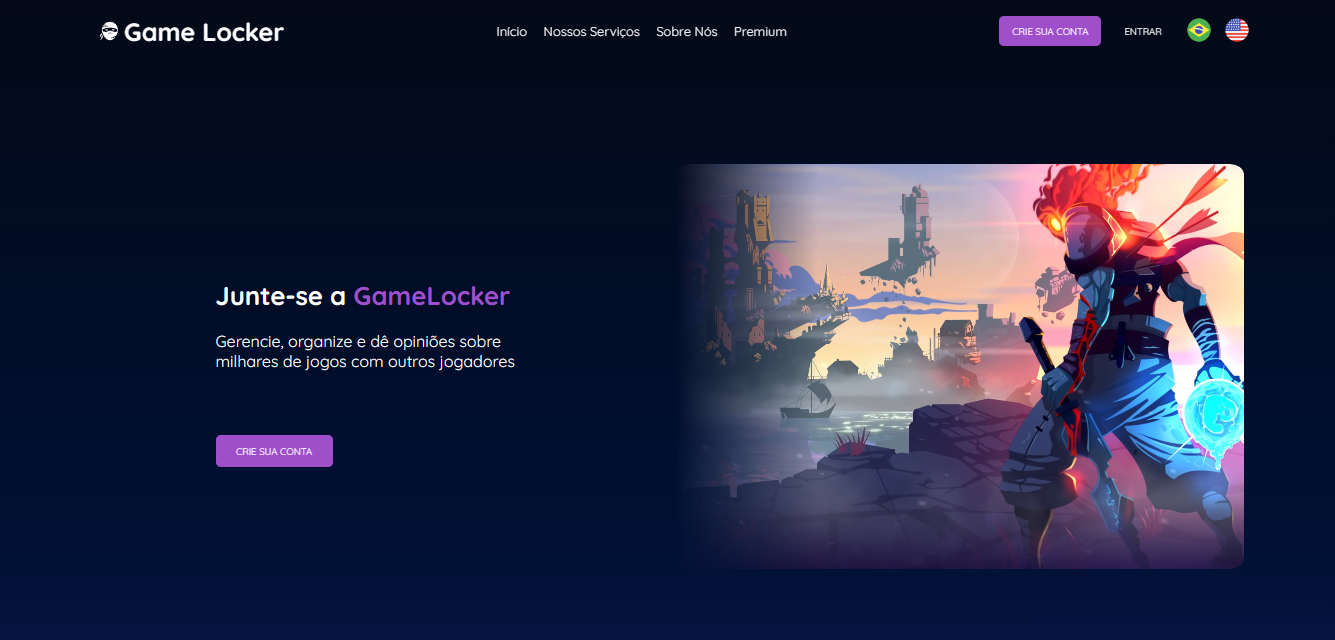
\includegraphics[width=1\textwidth,keepaspectratio]{./imagens/PrototipoLandingPage.png}
	\caption{Protótipo Landing Page 1}
	Fonte: Os autores
    \label{prototipoLandingPage}
\end{figure}
\pagebreak

Na Figura \ref{prototipoLandingPage2} é apresentado o protótipo da 2º parte da tela de Landing Page.

\begin{figure}[H]
	\centering
	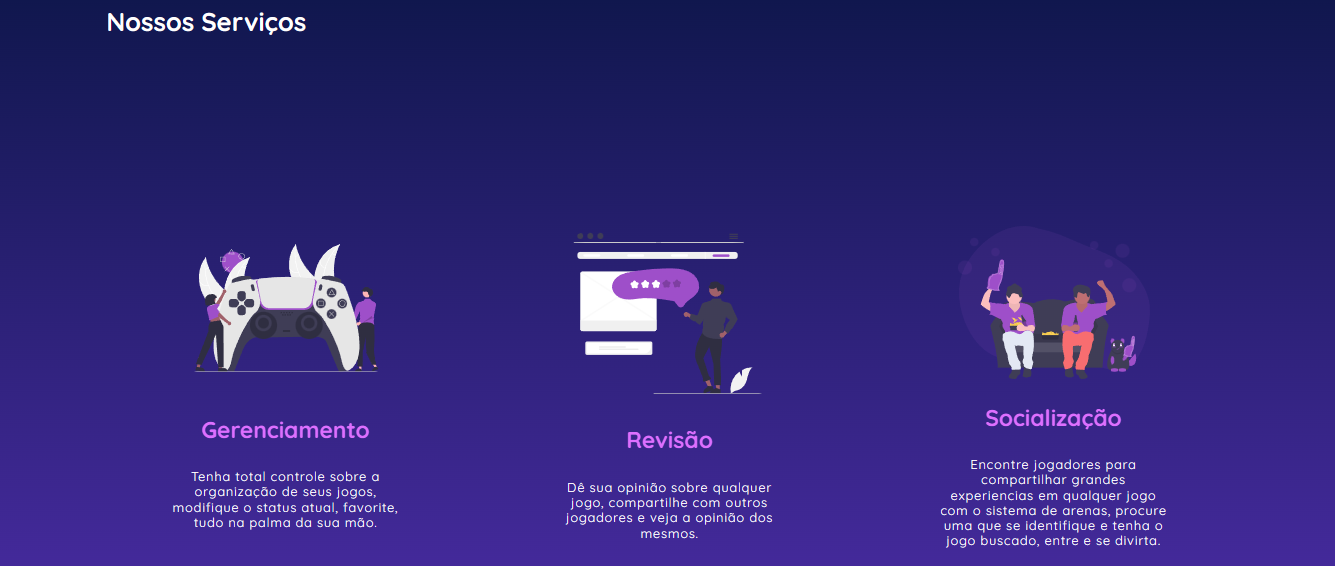
\includegraphics[width=1\textwidth,keepaspectratio]{./imagens/PrototipoLandingPage2.png}
	\caption{Protótipo Landing Page 2}
	Fonte: Os autores
    \label{prototipoLandingPage2}
\end{figure}

Na Figura \ref{prototipoLandingPage3} é apresentado o protótipo da 3º parte da tela de Landing Page.

\begin{figure}[H]
	\centering
	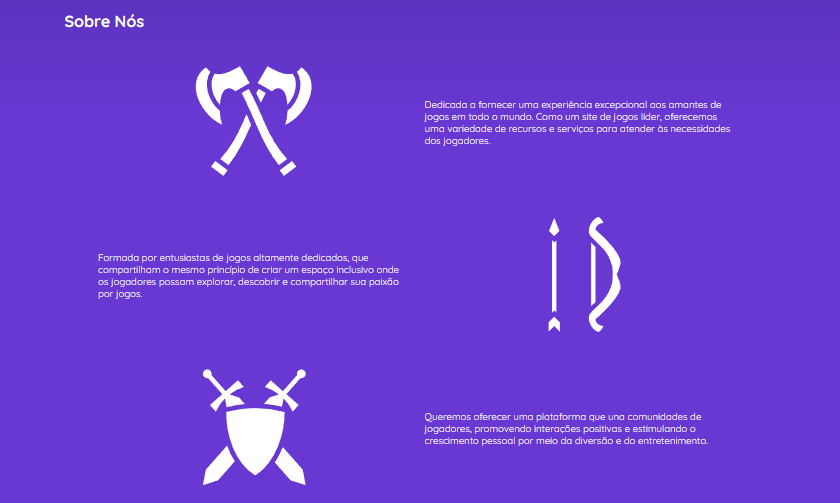
\includegraphics[width=1\textwidth,keepaspectratio]{./imagens/PrototipoLandingPage3.png}
	\caption{Protótipo Landing Page 3}
	Fonte: Os autores
    \label{prototipoLandingPage3}
\end{figure}
\pagebreak

Na Figura \ref{prototipoLandingPage4} é apresentado o protótipo da 4º parte da tela de Landing Page.

\begin{figure}[H]
	\centering
	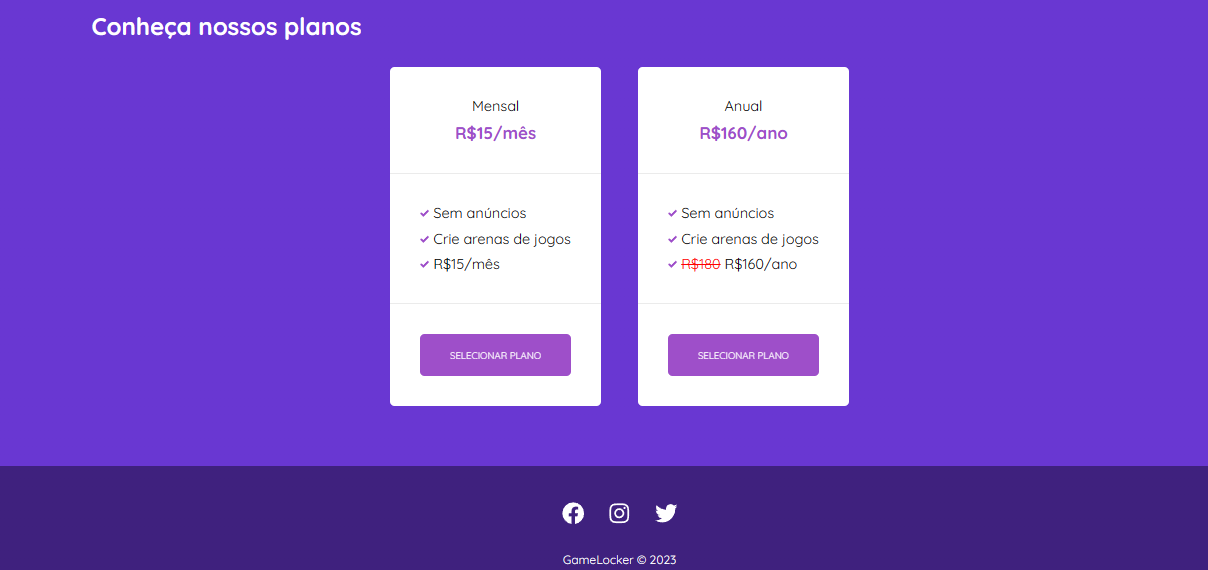
\includegraphics[width=1\textwidth,keepaspectratio]{./imagens/PrototipoLandingPage4.png}
	\caption{Protótipo Landing Page 4}
	Fonte: Os autores
    \label{prototipoLandingPage4}
\end{figure}

Na Figura \ref{prototipoCadastro} é apresentado o protótipo da tela de Cadastro.

\begin{figure}[H]
	\centering
	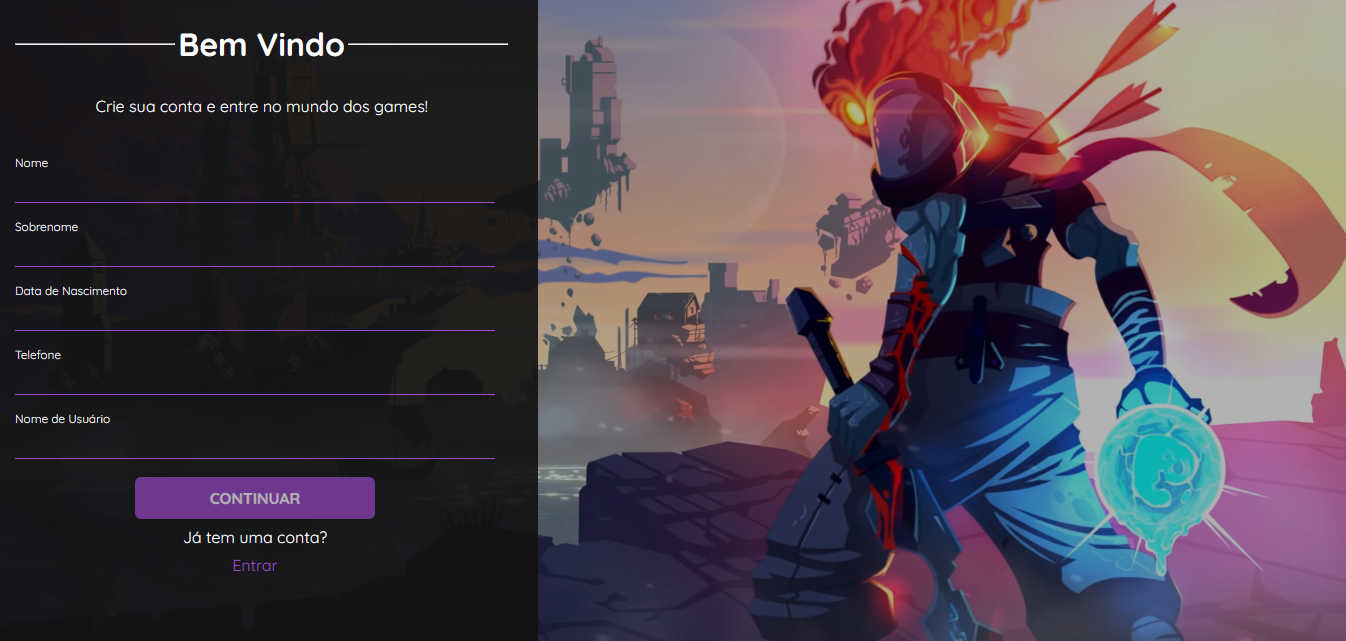
\includegraphics[width=1\textwidth,keepaspectratio]{./imagens/PrototipoCadastro.png}
	\caption{Protótipo Cadastro}
	Fonte: Os autores
    \label{prototipoCadastro}
\end{figure}
\pagebreak

Na Figura \ref{prototipoLogin} é apresentado o protótipo da tela de Login.

\begin{figure}[H]
	\centering
	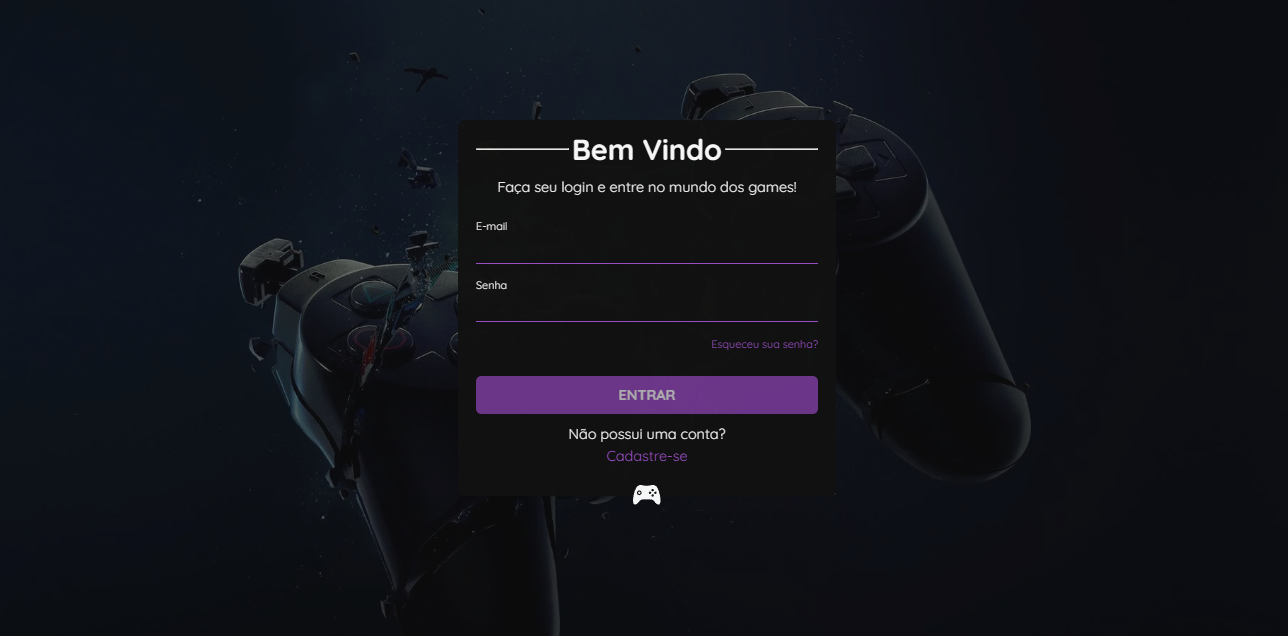
\includegraphics[width=1\textwidth,keepaspectratio]{./imagens/PrototipoLogin.png}
	\caption{Protótipo Login}
	Fonte: Os autores
    \label{prototipoLogin}
\end{figure}

Na Figura \ref{prototipoPortal} é apresentado o protótipo da 1º parte da tela do Portal.

\begin{figure}[H]
	\centering
	\includegraphics[width=1\textwidth,keepaspectratio]{./imagens/PrototipoPortal.png}
	\caption{Protótipo Portal 1}
	Fonte: Os autores
 \label{prototipoPortal}
\end{figure}
\pagebreak

Na Figura \ref{prototipoPortal2} é apresentado o protótipo da 2º parte da tela do Portal.

\begin{figure}[H]
	\centering
	\includegraphics[width=1\textwidth,keepaspectratio]{./imagens/PrototipoPortal2.png}
	\caption{Protótipo Portal 2}
	Fonte: Os autores
 \label{prototipoPortal2}
\end{figure}
\pagebreak

Na Figura \ref{prototipoPortal3} é apresentado o protótipo da 3º parte da tela do Portal.

\begin{figure}[H]
	\centering
	\includegraphics[width=1\textwidth,keepaspectratio]{./imagens/PrototipoPortal3.png}
	\caption{Protótipo Portal 3}
	Fonte: Os autores
 \label{prototipoPortal3}
\end{figure}
\pagebreak

Na Figura \ref{prototipoReview} é apresentado o protótipo do modal de Review.

\begin{figure}[H]
	\centering
	\includegraphics[scale=0.7]{./imagens/PrototipoReview.png}
	\caption{Protótipo Review}
	Fonte: Os autores
    \label{prototipoReview}
\end{figure}
\pagebreak

Na Figura \ref{prototipoMeuPerfil} é apresentado o protótipo da tela do Meu Perfil.

\begin{figure}[H]
	\centering
	\includegraphics[scale=0.34]{./imagens/PrototipoMeuPerfil.png}
	\caption{Protótipo Meu Perfil}
	Fonte: Os autores
    \label{prototipoMeuPerfil}
\end{figure}

Na Figura \ref{prototipoMeuJogos} é apresentado o protótipo da tela do Meu Jogos.

\begin{figure}[H]
	\centering
	\includegraphics[scale=0.45]{./imagens/PrototipoMeuJogos.png}
	\caption{Protótipo Meu Jogos}
	Fonte: Os autores
    \label{prototipoMeuJogos}
\end{figure}
\pagebreak

Na Figura \ref{prototipoPagamento} é apresentado o protótipo da tela de Pagamento.

\begin{figure}[H]
	\centering
	\includegraphics[scale=0.45]{./imagens/PrototipoPagamento.png}
	\caption{Protótipo Pagamento}
	Fonte: Os autores
    \label{prototipoPagamento}
\end{figure}
\pagebreak

Na Figura \ref{prototipoArena} é apresentado o protótipo da 1º parte da tela da Arena.

\begin{figure}[H]
	\centering
	\includegraphics[scale=0.45]{./imagens/PrototipoArena.png}
	\caption{Protótipo Arena}
	Fonte: Os autores
    \label{prototipoArena}
\end{figure}

Na Figura \ref{prototipoArena2} é apresentado o protótipo da 2º parte da tela da Arena.

\begin{figure}[H]
	\centering
	\includegraphics[scale=0.45]{./imagens/PrototipoArena2.png}
	\caption{Protótipo Arena 2}
	Fonte: Os autores
    \label{prototipoArena2}
\end{figure}
\pagebreak

Na Figura \ref{prototipoEncontrarAmigos} é apresentado o protótipo da 1º parte da tela de Encontrar Amigos.

\begin{figure}[H]
	\centering
	\includegraphics[scale=0.45]{./imagens/PrototipoEncontrarAmigos.png}
	\caption{Protótipo Encontrar Amigos}
	Fonte: Os autores
    \label{prototipoEncontrarAmigos}
\end{figure}

Na Figura \ref{prototipoEncontrarAmigos2} é apresentado o protótipo da 2º parte da tela de Encontrar Amigos

\begin{figure}[H]
	\centering
	\includegraphics[scale=0.45]{./imagens/PrototipoEncontrarAmigos2.png}
	\caption{Protótipo Encontrar Amigos 2}
	Fonte: Os autores
    \label{prototipoEncontrarAmigos2}
\end{figure}
\pagebreak

\chapter{Reuniões}
\label{ata-reunião}

\section{Reunião 1 - (04/03/2023)}
Com as equipes criadas, foram elencados principais pontos a se pensar:

\begin{itemize}
    \item Dias de Reunião
    \item Tema principal
    \item Tecnologias a serem utilizadas
    \item Funções básicas de cada membro
\end{itemize}

\section{Reunião 2 - (11/03/2023)}
Após a definição do tema do projeto, iniciou-se o processo de concepção, incluindo a criação de um protótipo de baixa fidelidade, considerando as funcionalidades a serem implementadas, o layout e, simultaneamente, preparou-se uma apresentação inicial.

Após uma análise minuciosa, a equipe optou por adotar o Kanban como metodologia de gerenciamento, visando assegurar um fluxo eficiente e organizado no desenvolvimento do projeto. Além disso, foram realizados preparativos para abranger as atividades requeridas, incluindo a criação de um canal no \textit{\gls{Youtube}}, e a implementação de controle de versão utilizando SVN, entre outras práticas necessárias.

\section{Reunião 3 - (18/03/2023)}
Foi realizada uma discussão detalhada para explicitar as funções de cada membro da equipe, buscando uma organização clara e eficiente. Além disso, a documentação foi aprimorada com base nos \textit{feedbacks} recebidos, visando uma execução do projeto que atendesse às expectativas de ambas as partes envolvidas, resultando em um trabalho no qual todos estivessem satisfeitos.

\section{Reunião 4 - (25/03/2023)}
A equipe dedicou seu esforço à estruturação do projeto, dividindo as responsabilidades entre as áreas de \textit{\gls{Front-end}}, \textit{\gls{Back-end}} e Banco de Dados. O foco principal foi estabelecer uma comunicação eficiente entre essas áreas, garantindo uma integração harmoniosa. 

Com as funções de cada membro claramente definidas durante a reunião anterior, o desenvolvimento foi iniciado de maneira simplificada. Simultaneamente, a equipe realizou outras atividades requisitadas, garantindo uma abordagem multitarefa para maximizar a eficiência do projeto.

\section{Reunião 5 - (01/04/2023)}
Nesta reunião, a equipe concentrou-se no desenvolvimento do desenho do projeto, o que incluiu a criação da arquitetura a ser utilizada, o Modelo Entidade-Relacionamento (MER) e o Diagrama Entidade-Relacionamento (DER). Foi dedicado tempo para planejar e visualizar a estrutura do sistema, mapeando as relações entre as entidades e definindo a organização dos dados. Simultaneamente, a equipe manteve-se atualizada com todas as outras dependências requisitadas, garantindo que o projeto estivesse alinhado com todas as exigências e expectativas estabelecidas.

\section{Reunião 6 - (08/04/2023)}
Nesta reunião, a equipe se dedicou a discutir os \textit{feedbacks} recebidos sobre a documentação, analisando as sugestões fornecidas e identificando as melhores abordagens para aprimorá-la. Durante essa análise, foram discutidas maneiras de evoluir a documentação, incorporando as sugestões relevantes e garantindo que estivesse completa e precisa.

Além disso, a equipe trabalhou na criação da identidade do projeto, deliberando sobre um nome definitivo, desenvolvendo logos e selecionando as cores que seriam utilizadas. Concomitantemente, atendendo à solicitação, a equipe iniciou o processo de criação do desenho da aplicação. Esse passo foi crucial para preparar uma apresentação futura, possibilitando uma visualização clara e detalhada do layout da aplicação que seria desenvolvida.

\section{Reunião 7 - (15/04/2023)}
Nesta reunião, os pontos destacados na documentação foram cuidadosamente abordados e resolvidos, garantindo que a documentação estivesse completa, precisa e atendesse aos padrões exigidos. Além disso, o desenvolvimento do Desenho da Aplicação continuou, com a equipe se esforçando para aprimorá-lo com base nos \textit{feedbacks} recebidos durante as aulas e ao tirar dúvidas.

Paralelamente, a equipe prosseguiu com a criação do projeto, incluindo o desenvolvimento da API que seria utilizada como parte do \textit{\gls{Back-end}} do sistema. Ao mesmo tempo, o \textit{\gls{Front-end}} da aplicação também estava sendo elaborado, permitindo uma visão mais clara e tangível do objetivo do projeto. 

\section{Reunião 8 - (22/04/2023)}
Após a conclusão do Desenho da Aplicação, a equipe deu início ao desenvolvimento da Prova de Conceito (POC). Durante esse período, houve um esforço contínuo para aprimorar a documentação, revisar e melhorar as arquiteturas estabelecidas e incorporar ideias provenientes tanto dos \textit{feedbacks} fornecidos pelo professor quanto das discussões entre os próprios membros da equipe.

\section{Reunião 9 - (29/04/2023)}
Nesta reunião, a equipe dedicou-se a uma análise detalhada da Prova de Conceito (POC), com o objetivo de identificar e corrigir qualquer erro ou problema existente. A revisão minuciosa visava minimizar o maior número de erros possível antes de considerar a POC como finalizada e pronta para entrega.

\section{Reunião 10 - (06/05/2023)}
Com a conclusão da Prova de Conceito (POC), a equipe deu início ao desenvolvimento do MVP (Mínimo Produto Viável) do projeto. Durante essa fase, houve um esforço conjunto para trabalhar na documentação, garantindo que estivesse atualizada e refletisse com precisão as últimas decisões e modificações feitas no projeto. Simultaneamente, foi elaborada uma lista inicial de funcionalidades que deveriam ser incluídas no MVP.

\begin{itemize}
    \item Funcionalidade de cadastro.
    \item Guardar Sessão de Login 
    \item Adicionar Reviews 
    \item Visualizar, editar e remover reviews.
    \item Filtragem de jogos no portal.
\end{itemize}

\section{Reunião 11 - (13/05/2023)}
A equipe começou a documentar a API utilizando a ferramenta Swagger, o que proporcionou uma documentação mais clara e organizada para os leitores. O Swagger é uma ferramenta poderosa que permite descrever, consumir e visualizar APIs de forma interativa. Isso não apenas facilitou a compreensão da API para os desenvolvedores, mas também proporcionou uma maneira eficiente de explorar e testar os \textit{\gls{Endpoints}} da API.

Além disso, a equipe continuou o desenvolvimento do código, implementando funcionalidades adicionais e fazendo melhorias contínuas na documentação à medida que novos requisitos e desafios eram descobertos durante o processo de desenvolvimento.

\section{Reunião 12 - (20/05/2023)}
Nesta reunião, a equipe concentrou-se em aprimorar todas as documentações já entregues e nas que ainda seriam entregues, visando fornecer uma base sólida e compreensível para o desenvolvimento do MVP (Mínimo Produto Viável). Durante o encontro, foram revisados detalhadamente os documentos existentes, buscando melhorar a clareza, precisão e abrangência das informações apresentadas.

\section{Reunião 13 - (27/05/2023)}
Na reunião realizada, o foco principal foi discutir o andamento atual do projeto. A equipe dedicou-se a identificar possíveis falhas ou pontos fracos no desenvolvimento até o momento. O objetivo era identificar áreas que precisavam de melhorias, correções ou otimizações.

\section{Reunião 14 - (03/06/2023)}
Durante a reunião, a equipe finalizou os slides para a Apresentação Final, realizando revisões por todos os membros para garantir que o conteúdo estivesse coerente com o que foi requisitado. Cada detalhe foi cuidadosamente analisado para assegurar clareza e precisão nas informações apresentadas.

Além disso, foi dado um foco especial ao \textit{\gls{Front-end}} do projeto. Todas as funcionalidades necessárias foram revisadas para garantir que estivessem implementadas corretamente e apresentadas de forma clara e intuitiva para os usuários. A interface do usuário foi refinada para proporcionar uma experiência fluida e agradável, priorizando a usabilidade e a compreensão das funcionalidades.

\section{Reunião 15 - (10/06/2023)}
Na reunião desta semana, nossa equipe compartilhou os detalhes de duas atividades cruciais em que estivemos focados recentemente. Primeiramente, discutimos os ajustes no Deploy do Back-end da aplicação, descrevendo à otimização e aprimoramento da infraestrutura de hospedagem do sistema. 

Durante a reunião, enfatizamos nosso compromisso em garantir que a apresentação seja clara, concisa e impactante, destacando os pontos fortes do MVP e seu potencial para agregar valor aos usuários finais, \textit{stakeholders} e parceiros envolvidos no projeto.

\section{Reunião 16 - (31/07/2023)}
Na reunião desta semana, dedicamos nosso tempo à integração dos novos membros da equipe, realizando uma sessão especial para delineação das responsabilidades individuais de cada membro. Durante o encontro, conduzimos discussões detalhadas sobre as pendências do projeto, analisando cuidadosamente cada tarefa que ainda estava por ser concluída.

Com base nessas informações essenciais, colaboramos ativamente para elaborar um cronograma estruturado e detalhado que servirá como guia durante a construção do projeto. 

\section{Reunião 17 - (07/08/2023)}
Na reunião desta semana, nossa equipe concentrou-se em dois aspectos-chave do projeto: o aprimoramento do estudo financeiro e a conclusão da funcionalidade de confirmação de e-mail. Durante o encontro, realizamos uma análise detalhada do estudo financeiro, examinando todos os elementos financeiros do empreendimento. Discutimos o orçamento, identificamos áreas potenciais para economia e otimização de gastos e projetamos custos futuros.

Além disso, celebramos o sucesso da equipe na implementação da funcionalidade de confirmação de e-mail em nossa aplicação. Essa reunião foi fundamental para garantir que todos na equipe estivessem alinhados com as metas financeiras do projeto e cientes dos avanços técnicos realizados.

\section{Reunião 18 - (14/08/2023)}
Na reunião da semana, nossa equipe de projeto realizou uma sessão altamente produtiva, concentrando-se em duas frentes essenciais: o desenvolvimento das principais funcionalidades da aplicação e a preparação do ambiente para o \textit{Google AdSense}.

O encontro foi marcado por discussões detalhadas e decisões cruciais. Iniciamos com uma análise cuidadosa das ferramentas e tecnologias necessárias para criar a Arena de Jogos. Simultaneamente, dedicamos uma parte significativa da reunião à preparação do ambiente para o \textit{Google AdSense}. 

\section{Reunião 19 - (21/08/2023)}
Na reunião realizada, nossa equipe de projeto seguiu um plano estruturado, focando em duas frentes cruciais para o progresso do projeto. Primeiramente, dedicamos uma parte significativa do tempo à revisão e aprimoramento detalhado da documentação do projeto. 

Simultaneamente, nos dedicamos ao aprofundamento do entendimento do sistema de pagamento. Realizamos uma análise dos requisitos técnicos, exploramos as ferramentas utilizadas no sistema, avaliamos cuidadosamente as considerações de segurança e absorvemos as melhores práticas relacionadas.

\section{Reunião 20 - (28/08/2023)}
Na reunião, nossa equipe focou seus esforços em duas áreas vitais do projeto. Primeiramente, dedicamos tempo ao aprimoramento da interface e dos \textit{\gls{Endpoints}} da Arena de Jogos. Discutimos melhorias específicas para garantir uma experiência de usuário mais intuitiva e eficaz. Cada membro da equipe compartilhou suas ideias e sugestões para enriquecer a navegação na plataforma.

Simultaneamente, investimos parte da reunião na pesquisa e avaliação de alternativas para a incorporação de anúncios em nosso sistema. Discutimos os obstáculos encontrados e começamos a considerar outras opções criativas para a monetização do projeto.

\section{Reunião 21 - (04/09/2023)}
Durante a reunião planejada, nossa equipe elaborou um plano estratégico abrangente para impulsionar o desenvolvimento da Arena de Jogos. Definimos claramente nossos objetivos, priorizando a implementação bem-sucedida do recurso de chat e os pequenos detalhes que precisavam ser resolvidos e delineamos um cronograma para a implementação do \textit{webhook}. Além disso, dedicamos uma parte significativa da reunião ao aprimoramento do processo de redefinição de senha. 

\section{Reunião 22 - (11/09/2023)}
Na reunião, iniciamos com um marco importante: a implementação do \textit{Webhook} na Arena de Jogos. Esse progresso significativo não apenas visa aprimorar a experiência dos jogadores, mas também elevar a funcionalidade da arena, permitindo uma comunicação mais eficiente e interativa entre os participantes, tornando-a ainda mais envolvente e dinâmica para os jogadores. Além disso, discutimos detalhadamente e confirmamos nossa estratégica decisão de adotar a API do Mercado Pago como o principal \textit{gateway} de pagamento em nossa plataforma.

\section{Reunião 23 - (18/09/2023)}
Durante a reunião, nossa equipe estabeleceu um plano detalhado para a implementação do \textit{Checkout} do Mercado Pago em nossa plataforma. Primeiramente, analisamos as características específicas do \textit{Checkout} do Mercado Pago e sua integração perfeita em nossa plataforma existente. Identificamos as opções de pagamento oferecidas e discutimos como elas atenderão às diversas necessidades dos nossos usuários. 

\section{Reunião 24 - (25/09/2023)}
Durante a reunião planejada desta semana, nossa equipe delineou um plano estratégico detalhado para o desenvolvimento do \textit{Checkout} do Mercado Pago. Iniciamos a reunião concentrando-nos na conclusão bem-sucedida da estrutura base do \textit{Checkout} do Mercado Pago. Cada membro da equipe recebeu tarefas específicas para aprimorar a interface do usuário e garantir uma integração perfeita com o Mercado Pago. Durante nossas discussões, enfocamos os detalhes técnicos e os requisitos específicos da integração, identificando áreas de possível melhoria.

Além disso, planejamos cuidadosamente a fase de testes do \textit{\gls{Back-end}}. Estabelecemos uma estratégia detalhada para conduzir testes unitários abrangentes, visando identificar e resolver qualquer problema potencial antes que ele afete a experiência do usuário final. Definimos critérios claros de aceitação e criamos um cronograma para garantir que todos os testes sejam concluídos dentro do prazo estabelecido.

\section{Reunião 25 - (02/10/2023)}
Na nossa última reunião, discutimos as próximas etapas para melhorar nosso sistema em três áreas cruciais: atualizações na documentação da entrega final, testes de segurança e implementação da opção de assinatura anual para nossos clientes.

\section{Reunião 26 - (09/10/2023)}
Durante a reunião, nossa equipe adotou revisou as prioridades do projeto e identificamos as áreas que precisavam de atenção imediata. Destacando as principais áreas de foco: testes unitários, usabilidade e documentação.

Decidimos dedicar uma parte significativa do nosso tempo na cobertura dos testes unitários. Atribuímos novos membros da equipe para auxiliar nessa tarefa, e estabelecemos critérios claros para a aceitação dos testes, garantindo que eles fossem abrangentes e rigorosos.

No que diz respeito à usabilidade, decidimos criar um formulário intuitivo que permitisse aos usuários avaliar a experiência do nosso projeto. Discutimos os elementos que deveriam estar presentes no formulário, incluindo perguntas específicas sobre a facilidade de navegação, a clareza das informações e a eficácia geral da aplicação. Quanto à documentação, revisamos os documentos existentes e identificamos áreas que precisavam ser atualizadas ou expandidas. E por fim, subir os arquivos pendentes ao SVN.

\section{Reunião 27 - (16/10/2023)}
Na reunião, ficou estabelecido que as métricas do GitHub serão desenvolvidas nesta semana. Identificamos uma urgente necessidade de implementar novas rotas de usuário, com o objetivo de disponibilizar novas informações do usuário na interface, bem como permitir uma visualização detalhada dos perfis, incluindo seus status dos jogos e suas reviews. Durante nossa discussão, enfatizamos a importância imediata de corrigir os bugs identificados na arena de jogos e disponibilizar o formulário de usabilidade para um público mais amplo.

\section{Reunião 28 - (23/10/2023)}
Durante a reunião, foram estabelecidas metas para concluir as etapas finais do projeto. Ficou decidido que a prioridade imediata é finalizar os testes unitários pendentes do back-end. Além disso, foi acordado a criação do Gource do desenvolvimento da entrega final, representação gráfica do histórico de desenvolvimento do projeto, mostrando a evolução do código e as contribuições individuais ao longo do tempo. Outro ponto destacado na reunião foi a necessidade de corrigir e atualizar a documentação do projeto de acordo com as sugestões apontadas pelo orientador, e foi decidido que a equipe se concentrará em organizar a apresentação final do projeto.

\chapter{Blog}
\label{postagens-blog}

Este apêndice apresenta as publicações realizadas no blog, tendo como objetivo documentar todo o processo de uma maneira formal e explícita.

Na Figura \ref{fig:109} é apresentada a primeira postagem do blog.

\begin{figure}[H]
	\centering
	\includegraphics[scale=0.68]{./imagens/Blog1.png}
	\caption{Blog - Postagem 1}
    \label{fig:109}
\end{figure}

Na Figura \ref{fig:110} é apresentada a segunda postagem do blog.

\begin{figure}[H]
	\centering
	\includegraphics[scale=0.68]{./imagens/Blog2.png}
	\caption{Blog - Postagem 2}
    \label{fig:110}
\end{figure}
\pagebreak

Na Figura \ref{fig:111} é apresentada a terceira postagem do blog.

\begin{figure}[H]
	\centering
	\includegraphics[scale=0.68]{./imagens/Blog3.png}
	\caption{Blog - Postagem 3}
    \label{fig:111}
\end{figure}

Na Figura \ref{fig:112} é apresentada a quarta postagem do blog.

\begin{figure}[H]
	\centering
	\includegraphics[scale=0.68]{./imagens/Blog4.png}
	\caption{Blog - Postagem 4}
    \label{fig:112}
\end{figure}
\pagebreak

Na Figura \ref{fig:113} é apresentada a quinta postagem do blog.

\begin{figure}[H]
	\centering
	\includegraphics[scale=0.68]{./imagens/Blog5.png}
	\caption{Blog - Postagem 5}
    \label{fig:113}
\end{figure}

Na Figura \ref{fig:114} é apresentada a sexta postagem do blog.

\begin{figure}[H]
	\centering
	\includegraphics[scale=0.68]{./imagens/Blog6.png}
	\caption{Blog - Postagem 6}
    \label{fig:114}
\end{figure}
\pagebreak

Na Figura \ref{fig:115} é apresentada a sétima postagem do blog.

\begin{figure}[H]
	\centering
	\includegraphics[scale=0.68]{./imagens/Blog7.png}
	\caption{Blog - Postagem 7}
    \label{fig:115}
\end{figure}
\pagebreak

Na Figura \ref{fig:116} é apresentada a oitava postagem do blog.

\begin{figure}[H]
	\centering
	\includegraphics[scale=0.68]{./imagens/Blog8.png}
	\caption{Blog - Postagem 8}
    \label{fig:116}
\end{figure}
\pagebreak

Na Figura \ref{fig:117} é apresentada a nona postagem do blog.

\begin{figure}[H]
	\centering
	\includegraphics[scale=0.68]{./imagens/Blog9.png}
	\caption{Blog - Postagem 9}
    \label{fig:117}
\end{figure}

Na Figura \ref{fig:118} é apresentada a décima postagem do blog.

\begin{figure}[H]
	\centering
	\includegraphics[scale=0.68]{./imagens/Blog10.png}
	\caption{Blog - Postagem 10}
    \label{fig:118}
\end{figure}
\pagebreak

Na Figura \ref{fig:119} é apresentada a undécima postagem do blog.

\begin{figure}[H]
	\centering
	\includegraphics[scale=0.68]{./imagens/Blog11.png}
	\caption{Blog - Postagem 11}
    \label{fig:119}
\end{figure}

Na Figura \ref{fig:120} é apresentada a duodécima postagem do blog.

\begin{figure}[H]
	\centering
	\includegraphics[scale=0.68]{./imagens/Blog12.png}
	\caption{Blog - Postagem 12}
    \label{fig:120}
\end{figure}
\pagebreak

Na Figura \ref{fig:121} é apresentada a décima terceira postagem do blog.

\begin{figure}[H]
	\centering
	\includegraphics[scale=0.68]{./imagens/Blog13.png}
	\caption{Blog - Postagem 13}
    \label{fig:121}
\end{figure}

Na Figura \ref{fig:122} é apresentada a décima quarta postagem do blog.

\begin{figure}[H]
	\centering
	\includegraphics[scale=0.68]{./imagens/Blog14.png}
	\caption{Blog - Postagem 14}
    \label{fig:122}
\end{figure}
\pagebreak

Na Figura \ref{fig:123} é apresentada a décima quinta postagem do blog.

\begin{figure}[H]
	\centering
	\includegraphics[scale=0.68]{./imagens/Blog15.png}
	\caption{Blog - Postagem 15}
    \label{fig:123}
\end{figure}

Na Figura \ref{fig:124} é apresentada a décima sexta postagem do blog.

\begin{figure}[H]
	\centering
	\includegraphics[scale=0.68]{./imagens/Blog16.png}
	\caption{Blog - Postagem 16}
    \label{fig:124}
\end{figure}
\pagebreak

Na Figura \ref{fig:125} é apresentada a décima sétima postagem do blog.

\begin{figure}[H]
	\centering
	\includegraphics[scale=0.68]{./imagens/Blog17.png}
	\caption{Blog - Postagem 17}
    \label{fig:125}
\end{figure}

Na Figura \ref{fig:126} é apresentada a décima oitava postagem do blog.

\begin{figure}[H]
	\centering
	\includegraphics[scale=0.68]{./imagens/Blog18.png}
	\caption{Blog - Postagem 18}
    \label{fig:126}
\end{figure}
\pagebreak

Na Figura \ref{fig:127} é apresentada a décima nona postagem do blog.

\begin{figure}[H]
	\centering
	\includegraphics[scale=0.68]{./imagens/Blog19.png}
	\caption{Blog - Postagem 19}
    \label{fig:127}
\end{figure}

Na Figura \ref{fig:128} é apresentada a vigésima postagem do blog.

\begin{figure}[H]
	\centering
	\includegraphics[scale=0.68]{./imagens/Blog20.png}
	\caption{Blog - Postagem 20}
    \label{fig:128}
\end{figure}
\pagebreak

Na Figura \ref{fig:129} é apresentada a vigésima primeira postagem do blog.

\begin{figure}[H]
	\centering
	\includegraphics[scale=0.68]{./imagens/Blog21.png}
	\caption{Blog - Postagem 21}
    \label{fig:129}
\end{figure}


Na Figura \ref{fig:130} é apresentada a vigésima segunda postagem do blog.

\begin{figure}[H]
	\centering
	\includegraphics[scale=0.68]{./imagens/Blog22.png}
	\caption{Blog - Postagem 22}
    \label{fig:130}
\end{figure}
\pagebreak

Na Figura \ref{fig:131} é apresentada a vigésima terceira postagem do blog.

\begin{figure}[H]
	\centering
	\includegraphics[scale=0.68]{./imagens/Blog23.png}
	\caption{Blog - Postagem 23}
    \label{fig:131}
\end{figure}

\chapter{Dicionário de Dados}
\label{DicionarioDados}

\begin{quadro}[h!]
\centering
\caption{AspNetUsers}
\label{tab:aspnetusers}
\begin{longtable}{|p{4cm}|p{2cm}|p{3cm}|p{5cm}|}
\hline
Campo & Chave & Tipo & Descrição
\\\hline
Id & PK & int & Identificador de um usuário
\\\hline
Phone & - & nvarchar(MAX) & Número de telefone do usuário
\\\hline
BirthDate & - & datetime & Data de nascimento do usuário
\\\hline
FirstName & - & nvarchar(MAX) & Primeiro nome do usuário
\\\hline
LastName & - & nvarchar(MAX) & Sobrenome do usuário
\\\hline
Email & - & nvarchar(256) & E-mail do usuário
\\\hline
UserName & - & nvarchar(256) & Nome de usuário
\\\hline
NormalizedUserName & - & nvarchar(256) & Sobrenome do usuário normalizado
\\\hline
NormalizedEmail & - & nvarchar(256) & E-mail do usuário normalizado
\\\hline
EmailConfirmed & - & bit & Controle para checar se o e-mail do usuário foi confirmado
\\\hline
PasswordHash & - & nvarchar(MAX) & Hash da senha
\\\hline
SecurityStamp & - & nvarchar(MAX) & Estado atual do usuário
\\\hline
ConcurrencyStamp & - & nvarchar(MAX) & Estado de criação do usuário
\\\hline
PhoneNumber & - & nvarchar(MAX) & Número de telefone do usuário
\\\hline
\end{longtable}
\fonte{Os Autores.}
\end{quadro}

\begin{quadro}[h!]
\centering
\caption{GameGenres}
\label{tab:gamegenres}
\begin{longtable}{|p{4cm}|p{2cm}|p{3cm}|p{5cm}|}
\hline
Campo & Chave & Tipo & Descrição
\\\hline
GameId & PK & int & Identificador composto para o Game
\\\hline
GenreId & PK & int & Identificador composto para o Genre
\\\hline
\end{longtable}
\fonte{Os Autores.}
\end{quadro}

\begin{quadro}[h!]
\centering
\caption{GamePlatforms}
\label{tab:gameplatforms}
\begin{longtable}{|p{4cm}|p{2cm}|p{3cm}|p{5cm}|}
\hline
Campo & Chave & Tipo & Descrição
\\\hline
GameId & PK & int & Identificador composto para o Game
\\\hline
PlatformId & PK & int & Identificador composto para a Platform
\\\hline
\end{longtable}
\fonte{Os Autores.}
\end{quadro}

\begin{quadro}[h!]
\centering
\caption{Games}
\label{tab:games}
\begin{longtable}{|p{4cm}|p{2cm}|p{3cm}|p{5cm}|}
\hline
Campo & Chave & Tipo & Descrição
\\\hline
Id & PK & int & Identificador para o jogo
\\\hline
ApiId & - & int & Identificador para o jogo na api externa
\\\hline
Name & - & nvarchar(MAX) & Nome do jogo
\\\hline
UrlImage & - & nvarchar(MAX) & Url da imagem do jogo
\\\hline
Metacritic & - & float & Nota do jogo no site Metacritic
\\\hline
ReleaseDate & - & datetime & Data de lançamento do jogo
\\\hline
\end{longtable}
\fonte{Os Autores.}
\end{quadro}

\begin{quadro}[h!]
\centering
\caption{Genres}
\label{tab:genres}
\begin{longtable}{|p{4cm}|p{2cm}|p{3cm}|p{5cm}|}
\hline
Campo & Chave & Tipo & Descrição
\\\hline
Id & PK & int & Identificador do gênero
\\\hline
EGenre & - & nvarchar(MAX) & Valor do gênero
\\\hline
\end{longtable}
\fonte{Os Autores.}
\end{quadro}

\begin{quadro}[h!]
\centering
\caption{Platforms}
\label{tab:platforms}
\begin{longtable}{|p{4cm}|p{2cm}|p{3cm}|p{5cm}|}
\hline
Campo & Chave & Tipo & Descrição
\\\hline
Id & PK & int & Identificador da plataforma
\\\hline
EPlatform & - & nvarchar(MAX) & Valor da plataforma
\\\hline
\end{longtable}
\fonte{Os Autores.}
\end{quadro}

\begin{quadro}[h!]
\centering
\caption{Reviews}
\label{tab:reviews}
\begin{longtable}{|p{4cm}|p{2cm}|p{3cm}|p{5cm}|}
\hline
Campo & Chave & Tipo & Descrição
\\\hline
Id & PK & int & Identificador da review
\\\hline
GameId & FK & int & Identificador do jogo presente na review
\\\hline
UserId & FK & int & Identificador do usuário responsável pela review
\\\hline
Score & - & int & Nota da review
\\\hline
Comment & - & nvarchar(MAX) & Comentário sobre o jogo
\\\hline
ReviewDate & - & datetime & Data de criação da review
\\\hline
GameStatus & - & int & Status do jogo
\\\hline
Favorite & - & bit & Controle para checar se o jogo está favoritado ou não
\\\hline
\end{longtable}
\fonte{Os Autores.}
\end{quadro}

\begin{quadro}[h!]
\centering
\caption{Subscriptions}
\label{tab:subscriptions}
\begin{longtable}{|p{4cm}|p{2cm}|p{3cm}|p{5cm}|}
\hline
Campo & Chave & Tipo & Descrição
\\\hline
Id & PK & int & Identificador da assinatura
\\\hline
IdPayer & - & int & Identificador do pagador da assinatura, na API do Mercado Pago
\\\hline
IdPlan & - & int & Identificador do plano, na API do Mercado Pago
\\\hline
StartDate & - & datetime & Data de Início da assinatura
\\\hline
LastPaymentDate & - & datetime & Data do último pagamento
\\\hline
IsActive & - & bit & Controle que indica se a assinatura está ativa
\\\hline
CancelDate & - & datetime & Data de cancelamento da assinatura, se houver
\\\hline
SubscriptionType & - & nvarchar(50) & Indica o tipo de assinatura (mensal ou anual)
\\\hline
UserId & FK & nvarchar(50) &Identificador do usuário ao qual a assinatura pertence
\\\hline
SubscriptionMPId & - & nvarchar(50) &Identificador da assinatura, na API do Mercado Pago
\\\hline
\end{longtable}
\fonte{Os Autores.}
\end{quadro}

\begin{quadro}[h!]
\centering
\caption{Payments}
\label{tab:payments}
\begin{longtable}{|p{4cm}|p{2cm}|p{3cm}|p{5cm}|}
\hline
Campo & Chave & Tipo & Descrição
\\\hline
Id & PK & int & Identificador do pagamento
\\\hline
PaymentDate & - & datetime & Data do pagamento
\\\hline
IdPayment & - & int & Identificador do pagamento, na API do Mercado Pago
\\\hline
SubscriptionId & FK & int & Identificador da assinatura
\\\hline
IdSubscription & - & int & Identificador da assinatura, na API do Mercado Pago
\\\hline
\end{longtable}
\fonte{Os Autores.}
\end{quadro}

\chapter{Métricas}
\label{Métricas}

Este apêndice apresenta as estatísticas relacionadas aos repositórios do projeto no GitHub, utilizando a ferramenta gitStats.

Na Figura \ref{generalFrontend} são apresentados os dados gerais do repositório GitHub referentes ao front-end.

\begin{figure}[H]
	\centering
	\includegraphics[scale=0.8]{./imagens/metricas/gitStatsFrontend/gitStatsGeneral.png}
	\caption{Dados Gerais do Repositório Front-end}
	Fonte: Os autores
    \label{generalFrontend}
\end{figure}
\pagebreak

Na Figura \ref{weeklyActivityFrontend} são apresentadas as estatísticas de atividade semanal do repositório GitHub referentes ao \textit{front-end}.

\begin{figure}[H]
	\centering
	\includegraphics[scale=0.7]{./imagens/metricas/gitStatsFrontend/activity/weeklyActivity.png}
	\caption{Atividade semanal do Repositório Front-end}
	Fonte: Os autores
    \label{weeklyActivityFrontend}
\end{figure}

Na Figura \ref{hourOfDayFrontend}, são apresentadas as estatísticas de \textit{commits} por hora do dia do repositório GitHub relacionadas ao \textit{front-end}.

\begin{figure}[H]
	\centering
	\includegraphics[scale=0.7]{./imagens/metricas/gitStatsFrontend/activity/hourOfDay.png}
	\caption{\textit{Commits} por hora do dia do Repositório Front-end}
	Fonte: Os autores
    \label{hourOfDayFrontend}
\end{figure}
\pagebreak

Na Figura \ref{hourOfWeekFrontend}, são apresentadas as estatísticas de \textit{commits} por hora da semana do repositório GitHub relacionadas ao \textit{front-end}.

\begin{figure}[H]
	\centering
	\includegraphics[scale=1]{./imagens/metricas/gitStatsFrontend/activity/hourOfWeek.png}
	\caption{\textit{Commits} por hora da semana do Repositório Front-end}
	Fonte: Os autores
    \label{hourOfWeekFrontend}
\end{figure}

Na Figura \ref{dayOfWeekFrontend}, são apresentadas as estatísticas de \textit{commits} por dia da semana do repositório GitHub relacionadas ao \textit{front-end}.

\begin{figure}[H]
	\centering
	\includegraphics[scale=0.7]{./imagens/metricas/gitStatsFrontend/activity/dayOfWeek.png}
	\caption{\textit{Commits} por dia da semana do Repositório Front-end}
	Fonte: Os autores
    \label{dayOfWeekFrontend}
\end{figure}
\pagebreak

Na Figura \ref{monthOfYearFrontend}, são apresentadas as estatísticas de \textit{commits} por mês do ano do repositório GitHub relacionadas ao \textit{front-end}.

\begin{figure}[H]
	\centering
	\includegraphics[scale=0.7]{./imagens/metricas/gitStatsFrontend/activity/monthOfYear.png}
	\caption{\textit{Commits} por mês do ano do Repositório Front-end}
	Fonte: Os autores
    \label{monthOfYearFrontend}
\end{figure}

Na Figura \ref{commitsFrontend}, são apresentadas as estatísticas de \textit{commits} por ano/mês do repositório GitHub relacionadas ao \textit{front-end}.

\begin{figure}[H]
	\centering
	\includegraphics[scale=0.6]{./imagens/metricas/gitStatsFrontend/activity/commits.png}
	\caption{\textit{Commits} por ano/mês do Repositório Front-end}
	Fonte: Os autores
    \label{commitsFrontend}
\end{figure}
\pagebreak

Na Figura \ref{listOfAuthorsFrontend}, é apresentada a lista dos autores do repositório GitHub relacionadas ao \textit{front-end}.

\begin{figure}[H]
	\centering
	\includegraphics[scale=0.7]{./imagens/metricas/gitStatsFrontend/authors/listOfAuthors.png}
	\caption{Lista dos autores do Repositório Front-end}
	Fonte: Os autores
    \label{listOfAuthorsFrontend}
\end{figure}

Na Figura \ref{cumulatedLinesFrontend}, são apresentadas as linhas de código acumuladas do repositório GitHub relacionadas ao \textit{front-end}.

\begin{figure}[H]
	\centering
	\includegraphics[scale=0.7]{./imagens/metricas/gitStatsFrontend/authors/cumulatedLines.png}
	\caption{Linhas de código acumuladas do Repositório Front-end}
	Fonte: Os autores
    \label{cumulatedLinesFrontend}
\end{figure}
\pagebreak

Na Figura \ref{commitPerAuthorFrontend}, são apresentadas as estatísticas de \textit{commits} por autor do repositório GitHub relacionadas ao \textit{front-end}.

\begin{figure}[H]
	\centering
	\includegraphics[scale=0.7]{./imagens/metricas/gitStatsFrontend/authors/commitPerAuthor.png}
	\caption{\textit{Commits} por autor do Repositório Front-end}
	Fonte: Os autores
    \label{commitPerAuthorFrontend}
\end{figure}

Na Figura \ref{filesFrontend}, são apresentados os dados de arquivos do repositório GitHub relacionadas ao \textit{front-end}.

\begin{figure}[H]
	\centering
	\includegraphics[scale=1]{./imagens/metricas/gitStatsFrontend/files/files.png}
	\caption{Dados de arquivo do Repositório Front-end}
	Fonte: Os autores
    \label{filesFrontend}
\end{figure}
\pagebreak

Na Figura \ref{fileCountFrontend}, são apresentadas as estatísticas de contagem de arquivo por data do repositório GitHub relacionadas ao \textit{front-end}.

\begin{figure}[H]
	\centering
	\includegraphics[scale=0.8]{./imagens/metricas/gitStatsFrontend/files/fileCount.png}
	\caption{Contagem de arquivo por data do Repositório Front-end}
	Fonte: Os autores
    \label{fileCountFrontend}
\end{figure}

Na Figura \ref{extensionsFrontend}, são apresentadas as estatísticas de extensões do repositório GitHub relacionadas ao \textit{front-end}.

\begin{figure}[H]
	\centering
	\includegraphics[scale=1]{./imagens/metricas/gitStatsFrontend/files/extensions.png}
	\caption{Extensões do Repositório Front-end}
	Fonte: Os autores
    \label{extensionsFrontend}
\end{figure}
\pagebreak

Na Figura \ref{linesFrontend}, são apresentadas as estatísticas de linhas de código do repositório GitHub relacionadas ao \textit{front-end}.

\begin{figure}[H]
	\centering
	\includegraphics[scale=0.8]{./imagens/metricas/gitStatsFrontend/lines/linesOfCode.png}
	\caption{Linhas de código do Repositório Front-end}
	Fonte: Os autores
    \label{linesFrontend}
\end{figure}

Na Figura \ref{generalBackend} são apresentados os dados gerais do repositório GitHub referentes ao \textit{back-end}.

\begin{figure}[H]
	\centering
	\includegraphics[scale=0.8]{./imagens/metricas/gitStatsBackend/gitStatsGeneral.png}
	\caption{Dados Gerais do Repositório Back-end}
	Fonte: Os autores
    \label{generalBackend}
\end{figure}
\pagebreak

Na Figura \ref{weeklyActivityBackend} são apresentadas as estatísticas de atividade semanal do repositório GitHub referentes ao \textit{back-end}.

\begin{figure}[H]
	\centering
	\includegraphics[scale=0.7]{./imagens/metricas/gitStatsBackend/activity/weeklyActivity.png}
	\caption{Atividade semanal do Repositório Back-end}
	Fonte: Os autores
    \label{weeklyActivityBackend}
\end{figure}

Na Figura \ref{hourOfDayBackend}, são apresentadas as estatísticas de \textit{commits} por hora do dia do repositório GitHub relacionadas ao \textit{back-end}.

\begin{figure}[H]
	\centering
	\includegraphics[scale=0.7]{./imagens/metricas/gitStatsBackend/activity/hourOfDay.png}
	\caption{\textit{Commits} por hora do dia do Repositório Back-end}
	Fonte: Os autores
    \label{hourOfDayBackend}
\end{figure}
\pagebreak

Na Figura \ref{hourOfWeekBackend}, são apresentadas as estatísticas de \textit{commits} por hora da semana do repositório GitHub relacionadas ao \textit{back-end}.

\begin{figure}[H]
	\centering
	\includegraphics[scale=1]{./imagens/metricas/gitStatsBackend/activity/hourOfWeek.png}
	\caption{\textit{Commits} por hora da semana do Repositório Back-end}
	Fonte: Os autores
    \label{hourOfWeekBackend}
\end{figure}

Na Figura \ref{dayOfWeekBackend}, são apresentadas as estatísticas de \textit{commits} por dia da semana do repositório GitHub relacionadas ao \textit{back-end}.

\begin{figure}[H]
	\centering
	\includegraphics[scale=0.7]{./imagens/metricas/gitStatsBackend/activity/dayOfWeek.png}
	\caption{\textit{Commits} por dia da semana do Repositório Back-end}
	Fonte: Os autores
    \label{dayOfWeekBackend}
\end{figure}
\pagebreak

Na Figura \ref{monthOfYearBackend}, são apresentadas as estatísticas de \textit{commits} por mês do ano do repositório GitHub relacionadas ao \textit{back-end}.

\begin{figure}[H]
	\centering
	\includegraphics[scale=0.7]{./imagens/metricas/gitStatsBackend/activity/monthOfYear.png}
	\caption{\textit{Commits} por mês do ano do Repositório Back-end}
	Fonte: Os autores
    \label{monthOfYearBackend}
\end{figure}

Na Figura \ref{commitsBackend}, são apresentadas as estatísticas de \textit{commits} por ano/mês do repositório GitHub relacionadas ao \textit{back-end}.

\begin{figure}[H]
	\centering
	\includegraphics[scale=0.6]{./imagens/metricas/gitStatsBackend/activity/commits.png}
	\caption{\textit{Commits} por ano/mês do Repositório Back-end}
	Fonte: Os autores
    \label{commitsBackend}
\end{figure}
\pagebreak

Na Figura \ref{listOfAuthorsBackend}, é apresentada a lista dos autores do repositório GitHub relacionadas ao \textit{back-end}.

\begin{figure}[H]
	\centering
	\includegraphics[scale=0.65]{./imagens/metricas/gitStatsBackend/authors/listOfAuthors.png}
	\caption{Lista dos autores do Repositório Back-end}
	Fonte: Os autores
    \label{listOfAuthorsBackend}
\end{figure}

Na Figura \ref{cumulatedLinesBackend}, são apresentadas as linhas de código acumuladas do repositório GitHub relacionadas ao \textit{back-end}.

\begin{figure}[H]
	\centering
	\includegraphics[scale=0.7]{./imagens/metricas/gitStatsBackend/authors/cumulatedLines.png}
	\caption{Linhas de código acumuladas do Repositório Back-end}
	Fonte: Os autores
    \label{cumulatedLinesBackend}
\end{figure}
\pagebreak

Na Figura \ref{commitPerAuthorBackend}, são apresentadas as estatísticas de \textit{commits} por autor do repositório GitHub relacionadas ao \textit{back-end}.

\begin{figure}[H]
	\centering
	\includegraphics[scale=0.7]{./imagens/metricas/gitStatsBackend/authors/commitsPerAuthors.png}
	\caption{\textit{Commits} por autor do Repositório Back-end}
	Fonte: Os autores
    \label{commitPerAuthorBackend}
\end{figure}

Na Figura \ref{filesBackend}, são apresentados os dados de arquivos do repositório GitHub relacionadas ao \textit{back-end}.

\begin{figure}[H]
	\centering
	\includegraphics[scale=1]{./imagens/metricas/gitStatsBackend/files/files.png}
	\caption{Dados de arquivo do Repositório Back-end}
	Fonte: Os autores
    \label{filesBackend}
\end{figure}
\pagebreak

Na Figura \ref{fileCountBackend}, são apresentadas as estatísticas de contagem de arquivo por data do repositório GitHub relacionadas ao \textit{back-end}.

\begin{figure}[H]
	\centering
	\includegraphics[scale=0.8]{./imagens/metricas/gitStatsBackend/files/fileCount.png}
	\caption{Contagem de arquivo por data do Repositório Back-end}
	Fonte: Os autores
    \label{fileCountBackend}
\end{figure}

Na Figura \ref{extensionsBackend}, são apresentadas as estatísticas de extensões do repositório GitHub relacionadas ao \textit{back-end}.

\begin{figure}[H]
	\centering
	\includegraphics[scale=1]{./imagens/metricas/gitStatsBackend/files/extensions.png}
	\caption{Extensões do Repositório Back-end}
	Fonte: Os autores
    \label{extensionsBackend}
\end{figure}
\pagebreak

Na Figura \ref{linesBackend}, são apresentadas as estatísticas de linhas de código do repositório GitHub relacionadas ao \textit{back-end}.

\begin{figure}[H]
	\centering
	\includegraphics[scale=0.8]{./imagens/metricas/gitStatsBackend/lines/linesOfCode.png}
	\caption{Linhas de código do Repositório Back-end}
	Fonte: Os autores
    \label{linesBackend}
\end{figure}

\chapter{Termos e Condições}
\label{termos-e-condicoes}
\index{pdf}
\includepdf[pages= - ,scale=0.8,frame=true,pagecommand={}]{documentos/Termos_e_Condições.pdf}

\end{apendicesenv}
% ---


%% ----------------------------------------------------------
% Anexos
% Documentos gerados por outros autores
% ----------------------------------------------------------

% ---
% Inicia os anexos
% ---
%\begin{anexosenv}
%\anexos
% Imprime uma página indicando o início dos anexos
%\partanexos


% ----------------------------------------------------------
%\chapter{Nota dos headers}
% ----------------------------------------------------------

\begin{comment}
% ---
\chapter{Manual todonotes(parcial)}
\label{manual-todonotes}
% ---
\index{pdf}
% se pages = "-"  fica com arquivo completo
\includepdf[pages=1-3,scale=0.8,frame=true,pagecommand={}]{anexos/todonotes.pdf}

% ---
% Para incluir sem gerar a quebra de página inicial no anexo
\includepdf[pages=1,scale=0.7,frame=true,pagecommand=\chapter{Manual pdfpages(parcial)}\label{manual-pdfpages}]{anexos/pdfpages.pdf}
\includepdf[pages=2-3,scale=0.8,frame=true,pagecommand={}]{anexos/pdfpages.pdf}

% ---
\chapter{Manual acronym(parcial)}
\index{pdf}
% somente algumas páginas para exemplo sem borda
\includepdf[pages=1-3,frame=false,pagecommand={}]{anexos/acronym.pdf}



\includepdf[frame=true,scale=0.7,pagecommand=\chapter{Referência Rápida pifont}\label{pifont-quickref}]{anexos/pifont.pdf}
\end{comment}

%\end{anexosenv}


\end{document}